\chapter{Курсовое проектирование}

\section{Цели и задачи курсового проектирования}

Целью курсового проектирования является закрепление теоретических знаний, полученных при~изучении глав~1-4, и~освоение методики расчёта подшипников скольжения с~дискретным микрорельефом рабочей поверхности.

В~процессе выполнения курсовой работы студент должен:
\begin{itemize}
\item сформулировать расчётную задачу для~подшипника скольжения заданного типа;
\item записать математическую модель смазочного слоя на~основе уравнения Рейнольдса;
\item задать параметры микрорельефа (тип элементов, глубину, размеры, схему расположения);
\item выполнить расчёт характеристик гладкого подшипника;
\item выполнить расчёт характеристик подшипника с~микрорельефом;
\item провести сравнительный анализ результатов, сделать выводы об~эффективности текстурирования;
\item оформить результаты в~виде пояснительной записки.
\end{itemize}

В~результате выполнения работы студент приобретает навыки самостоятельного инженерного расчёта подшипниковых узлов, анализа и~интерпретации результатов моделирования, а~также оформления технической документации.


\section{Указания к выполнению курсовой работы}

Рекомендуемый алгоритм выполнения курсовой работы:

\begin{enumerate}
\item \textbf{Получение задания.} Выбрать вариант из~таблицы~\ref{tab:variants} (по~указанию преподавателя или~по~номеру в~списке группы). Записать исходные данные: тип подшипника, геометрические размеры, параметры смазки, режим работы, тип и~параметры микрорельефа.

\item \textbf{Формулировка математической модели.} На~основе материала глав~2-3 записать уравнение Рейнольдса для~заданного типа подшипника, граничные условия, условие кавитации. Определить функцию зазора для~гладкого и~текстурированного вариантов. Записать формулы для~вычисления интегральных характеристик (несущая способность, коэффициент трения, утечки).

\item \textbf{Расчёт гладкого подшипника.} Выполнить численный расчёт поля давления и~интегральных характеристик для~подшипника без~микрорельефа. Этот~расчёт является базовым (эталонным) для~последующего сравнения.

\item \textbf{Задание параметров микрорельефа.} В~соответствии с~вариантом задания определить геометрию элементов (глубину, размеры), схему расположения и~зону нанесения текстуры. Записать функцию добавки к~зазору~$\Delta h$.

\item \textbf{Расчёт текстурированного подшипника.} Выполнить численный расчёт с~учётом микрорельефа. Получить поля давления, кавитационные зоны и~интегральные характеристики.

\item \textbf{Сравнительный анализ.} Вычислить нормированные показатели эффективности (отношение характеристик текстурированного подшипника к~гладкому). Построить графики зависимостей. Проанализировать влияние параметров микрорельефа.

\item \textbf{Оформление пояснительной записки.} Оформить работу в~соответствии с~требованиями раздела~\ref{sec:requirements}.
\end{enumerate}


\section{Варианты курсовой работы}\label{sec:variants}

Варианты курсовой работы приведены в~таблице~\ref{tab:variants}. Каждый вариант определяет тип подшипника, основные размеры, режим работы, тип смазки и~параметры микрорельефа.

\begin{table}[!ht]
\centering
\caption{Варианты курсовой работы}
\label{tab:variants}
\small
\begin{tabularx}{\textwidth}{|c|X|c|c|c|c|c|}
\hline
\textbf{№} & \textbf{Тип подшипника} & $\boldsymbol{R}$, \textbf{мм} & $\boldsymbol{L}$, \textbf{мм} & $\boldsymbol{c}$, \textbf{мкм} & $\boldsymbol{n}$, \textbf{об/мин} & \textbf{Тип рельефа} \\
\hline
1  & Радиальный & 30 & 48 & 40 & 3000 & Лунки \\
\hline
2  & Радиальный & 35 & 56 & 50 & 2980 & Лунки \\
\hline
3  & Радиальный & 40 & 64 & 60 & 1500 & Лунки \\
\hline
4  & Радиальный & 25 & 40 & 35 & 6000 & Лунки \\
\hline
5  & Радиальный & 50 & 80 & 70 & 1000 & Канавки \\
\hline
6  & Радиальный & 30 & 40 & 60 & 120  & Лунки \\
\hline
7  & Радиальный & 35 & 50 & 45 & 4500 & Лунки \\
\hline
8  & Радиальный & 45 & 72 & 55 & 2000 & Канавки \\
\hline
9  & Радиальный & 30 & 48 & 40 & 3600 & Лунки \\
\hline
10 & Радиальный & 40 & 56 & 50 & 2500 & Лунки \\
\hline
11 & Упорный    & 30 & --  & 50 & 3000 & Лунки \\
\hline
12 & Упорный    & 40 & --  & 40 & 1500 & Лунки \\
\hline
13 & Упорный    & 50 & --  & 60 & 3600 & Канавки \\
\hline
14 & Упорный    & 35 & --  & 45 & 6000 & Лунки \\
\hline
15 & Упорный    & 25 & --  & 35 & 2000 & Лунки \\
\hline
\end{tabularx}
\end{table}

\FloatBarrier

\textit{Примечания к таблице~\ref{tab:variants}:}
\begin{itemize}
\item для~радиальных подшипников~$R$~-- радиус вала, $L$~-- длина подшипника, $c$~-- радиальный зазор;
\item для~упорных подшипников~$R$~-- внутренний радиус, наружный радиус $R_{\mathrm{out}} = 2R$, параметр клина $K = 2{,}0$, минимальный зазор~$h_{\mathrm{out}} = c$, число колодок~$N = 6$;
\item динамическая вязкость смазки для~всех вариантов $\mu = 0{,}01$~Па$\cdot$с (масло ISO~VG~32 при~$40\,^{\circ}$C), если иное не~указано преподавателем;
\item тип рельефа <<Лунки>>~-- эллипсоидальные лунки в~шахматной раскладке; <<Канавки>>~-- поперечные канавки параболического профиля;
\item безразмерная глубина элементов $H_p$, зона нанесения и~число элементов выбираются студентом самостоятельно на~основе рекомендаций, изложенных в~примерах данной главы.
\end{itemize}


\section{Требования к пояснительной записке и графическому материалу}\label{sec:requirements}

Пояснительная записка к~курсовой работе должна содержать следующие разделы:

\begin{enumerate}
\item Титульный лист (по~форме, установленной кафедрой).
\item Задание на~курсовую работу.
\item Содержание.
\item Введение: цель работы, краткое описание объекта исследования.
\item Исходные данные: параметры подшипника, смазки, микрорельефа (в~виде таблицы).
\item Математическая модель: уравнение Рейнольдса, граничные условия, функция зазора, интегральные функционалы.
\item Результаты расчёта гладкого подшипника: поля давления, интегральные характеристики, графики.
\item Результаты расчёта текстурированного подшипника: поля давления, интегральные характеристики, графики.
\item Сравнительный анализ: нормированные показатели эффективности, таблицы сравнения, графики.
\item Выводы: основные результаты, рекомендации.
\item Список использованных источников.
\end{enumerate}

\textbf{Объём} пояснительной записки~-- 25-40~страниц (без~приложений).

\textbf{Оформление}~-- в~соответствии с~СТУ~7.5-07-2021 СФУ: формат~A4, шрифт Times New Roman 14~пт, одинарный межстрочный интервал, поля: левое~-- 30~мм, правое~-- 10~мм, верхнее и~нижнее~-- 20~мм, абзацный отступ~-- 12,5~мм. Рисунки и~таблицы оформляются в~соответствии с~ГОСТ.

\textbf{Графический материал:}
\begin{itemize}
\item схема подшипника с~указанием основных размеров;
\item карта распределения зазора (для~текстурированного варианта);
\item поле давления для~гладкого и~текстурированного подшипников;
\item графики зависимостей интегральных характеристик;
\item диаграмма нормированных показателей эффективности.
\end{itemize}


\section{Пример анализа радиального подшипника скольжения центробежного насоса}

Ниже приведён подробный пример расчёта радиального подшипника скольжения ротора центробежного насоса. Пример демонстрирует полный цикл анализа: от~задания исходных данных через формулировку математической модели и~выполнение расчёта к~сравнению гладкого и~текстурированного вариантов и~формулированию выводов. Рекомендуется использовать данный пример как~образец при~выполнении курсовой работы для~радиального подшипника.

% =============================================================
% 5 Анализ радиального подшипника скольжения
%   центробежного насоса
% =============================================================
\chapter{Анализ рельефного радиального подшипника скольжения центробежного насоса}

\section{Объект исследования и исходные данные}

Объектом исследования в настоящей главе является радиальный
подшипник скольжения ротора центробежного насоса~\cite{bashmur2024a}.
Подшипниковый узел предназначен для восприятия радиальных
нагрузок, передаваемых от ротора к корпусу, и обеспечения
жидкостного режима смазки в рабочем диапазоне скоростей
и нагрузок.

Подшипник представляет собой цилиндрическую пару: вал
радиуса~$R$ вращается внутри вкладыша с радиальным зазором~$c$.
Относительный зазор $\psi = c/R$ определяет геометрическую
характеристику подшипника; отношение длины к диаметру~$L/D$
характеризует его осевую протяжённость. Рабочей средой является
масло с динамической вязкостью~$\mu_0$ при референсной
температуре~$T_0$. Вал вращается с угловой скоростью~$\omega$
и нагружен радиальной силой~$F_{\mathrm{ext}}$, действующей
в плоскости поперечного сечения.

Расчёт выполняется в изотермическом приближении: температура
смазки принята постоянной ($T = T_0$, $\mu = \mathrm{const}$),
что обосновано в разделе~4.2 при умеренных скоростях скольжения
и нагрузках, характерных для рассматриваемого узла. Плотность
смазки считается постоянной ($\rho = \mathrm{const}$),
поверхности~-- гладкими (обоснование~-- раздел~4.3).

Основные параметры подшипника сведены в таблицу~\ref{tab:journal_params}.

\begin{table}[!ht]
\centering
\caption{Параметры радиального подшипника скольжения}
\label{tab:journal_params}
\begin{tabularx}{\textwidth}{|X|c|c|c|}
\hline
\multicolumn{1}{|c|}{\textbf{Параметр}} & \textbf{Обозначение} & \textbf{Значение} & \textbf{Единица} \\
\hline
Радиус вала            & $R$              & 35{,}0  & мм \\
\hline
Длина подшипника       & $L$              & 56{,}0  & мм \\
\hline
Радиальный зазор       & $c$              & 50      & мкм \\
\hline
Относительный зазор    & $\psi = c/R$     & $1{,}43 \times 10^{-3}$ & -- \\
\hline
Отношение $L/D$        & $L/D$            & 0{,}80  & -- \\
\hline
Угловая скорость       & $\omega$         & 312{,}0 & рад/с \\
\hline
Динамическая вязкость  & $\mu_0$          & $1{,}105 \times 10^{-2}$ & Па$\cdot$с \\
\hline
Давление кавитации     & $p_{\mathrm{cav}}$ & 0     & Па \\
\hline
\end{tabularx}
\end{table}

\FloatBarrier

Схема подшипника в поперечном сечении представлена на
рисунке~\ref{fig:journal_scheme}.

\begin{figure}[!ht]
\centering
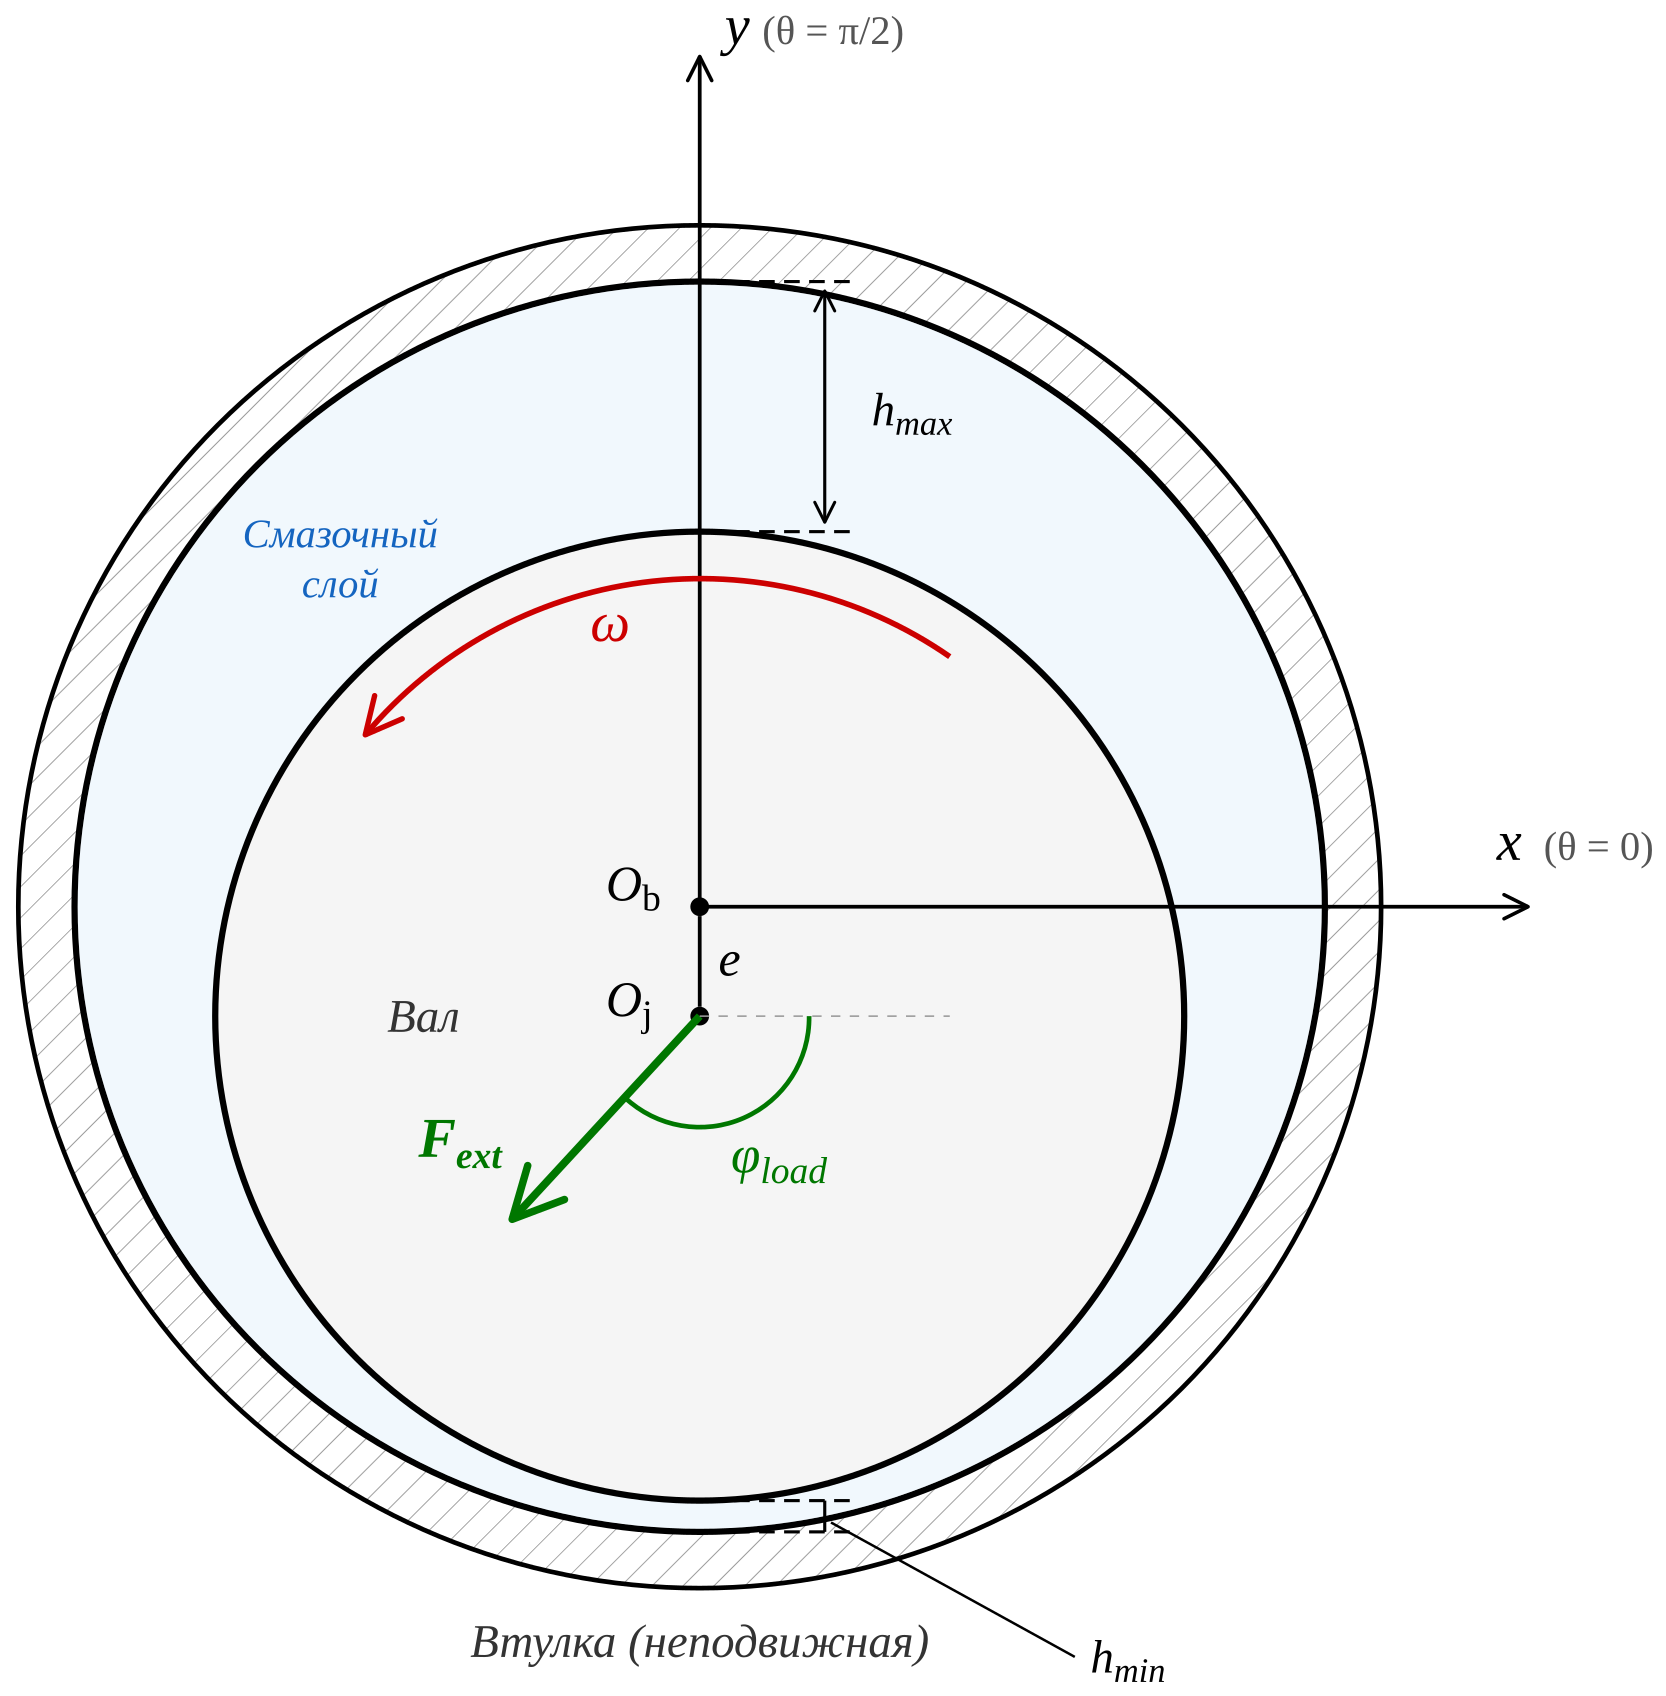
\includegraphics[width=\textwidth,height=0.9\textheight,keepaspectratio]{figures/ch05/fig_5_1.png}
\caption{Схема радиального подшипника скольжения центробежного насоса}
\label{fig:journal_scheme}
\end{figure}

\FloatBarrier

Обозначения на схеме соответствуют параметрам
таблицы~\ref{tab:journal_params}; направление отсчёта
угла~$\theta$ и положение начала координат определены
в разделе~\ref{sec:problem_statement_ch5}.

\section{Постановка задачи}\label{sec:problem_statement_ch5}

Расчётная область представляет собой развёрнутую поверхность
смазочного зазора $(\theta, z) \in [0,\,2\pi] \times [-L/2,\,L/2]$,
где $\theta$~-- окружная координата, $z$~-- осевая координата.
При переходе к безразмерным переменным (подраздел~2.1.6)
осевая координата нормируется на полудлину: $Z = 2z/L$,
так что $Z \in [-1,\,1]$.

В тексте главы окружная координата обозначается~$\theta$;
на рисунках ось подписана~$\varphi$; везде $\theta \equiv \varphi$.

Для гладкого цилиндрического подшипника безразмерная толщина
зазора определяется законом~\eqref{eq:journal_h}:
\begin{equation}
  H(\theta) = 1 + \varepsilon\cos\theta,
  \label{eq:journal_h_ch5}
\end{equation}
где $\varepsilon = e/c$~-- относительный эксцентриситет
($0 \leq \varepsilon < 1$), $e$~-- смещение оси вала
относительно оси вкладыша. При $\varepsilon = 0$ зазор
равномерный, при $\varepsilon \to 1$ минимальный зазор
$h_{\min} = c\,(1 - \varepsilon)$ стремится к нулю.

Для подшипника с детерминированными микроструктурами толщина
зазора записывается в виде суперпозиции~\eqref{eq:h_superposition}:
\begin{equation}
  H = H_{\mathrm{base}}(\theta) + \Delta H_{\mathrm{texture}}(\theta, Z),
  \label{eq:journal_h_tex_ch5}
\end{equation}
где $H_{\mathrm{base}} = 1 + \varepsilon\cos\theta$~-- базовый зазор
гладкого подшипника, $\Delta H_{\mathrm{texture}}$~-- добавка,
описывающая микрорельеф (подраздел~2.2, формула~\eqref{eq:journal_h_textured}).

Распределение давления в смазочном слое описывается безразмерным
уравнением Рейнольдса~\eqref{eq:reynolds_nondim} с параметром
анизотропии~$\Lambda$~\eqref{eq:nondim_Lambda}. Для радиального
подшипника $\Lambda = 2R/L$; данный параметр определяет
соотношение окружного и осевого масштабов задачи.

Кавитация учитывается по условию Рейнольдса: давление не допускается
ниже давления кавитации, т.е.\ $P \geq 0$; в области разрыва плёнки
принимается $P = 0$. Данное условие является упрощением постановки JFO
(\eqref{eq:jfo_conservation}, \eqref{eq:jfo_complementarity});
полная JFO-постановка составляет предмет дальнейшего развития модели.

Граничные условия задачи формулируются следующим образом:
по окружной координате~$\theta$ поле давления периодично
($P(\theta = 0) = P(\theta = 2\pi)$); на торцах подшипника
давление равно атмосферному ($P = 0$ при $Z = \pm 1$).

Допущения, принятые в настоящей главе, включают: изотермическое
приближение ($T = T_0$, обоснование~-- раздел~4.2), постоянство
плотности ($\rho = \mathrm{const}$, раздел~4.1) и гладкость
поверхностей ($\Delta h_{\mathrm{rough}} = 0$, раздел~4.3).

Расчётная область с граничными условиями схематически показана
на рисунке~\ref{fig:journal_domain}.

\begin{figure}[!ht]
\centering
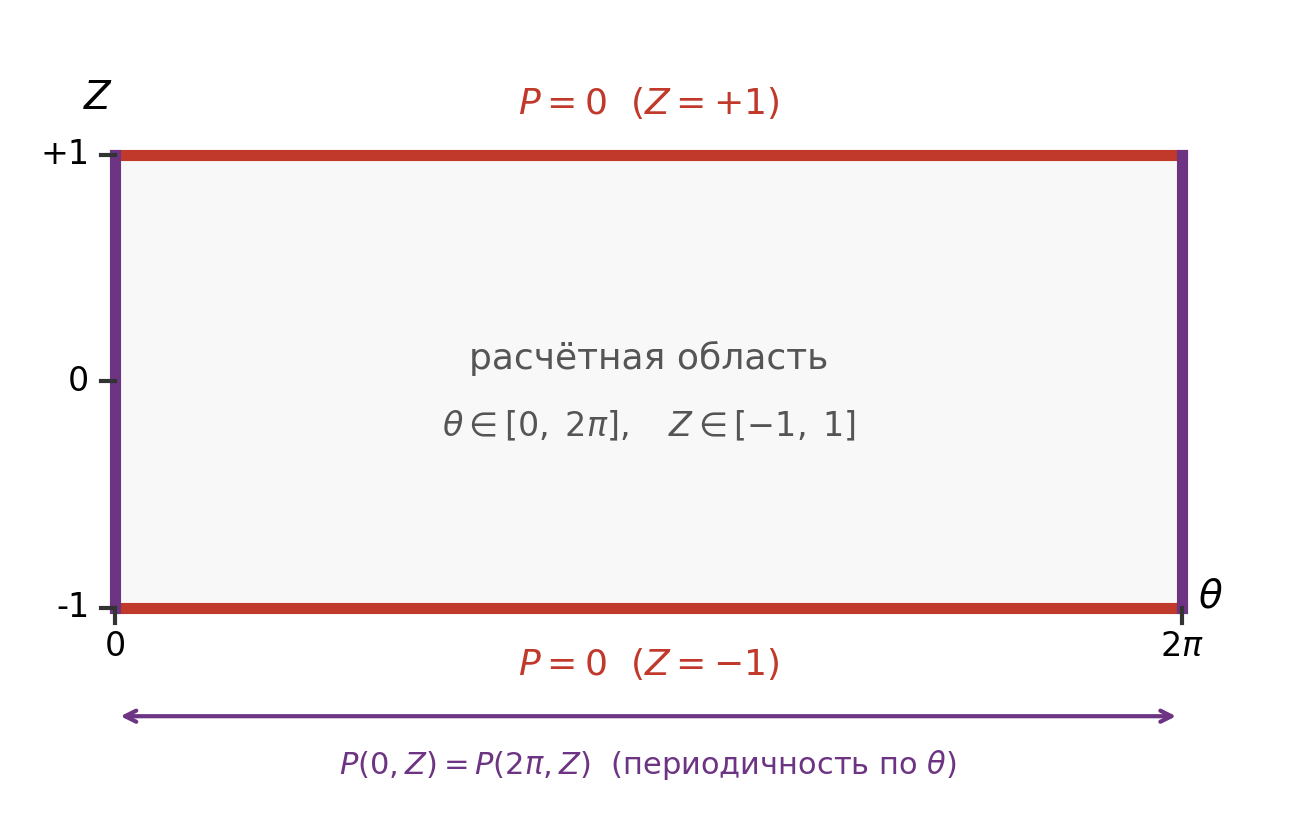
\includegraphics[width=\textwidth,height=0.9\textheight,keepaspectratio]{figures/ch05/fig_5_2.png}
\caption{Расчётная область $(\theta, Z) \in [0,\,2\pi] \times [-1,\,1]$
  и граничные условия: периодичность по~$\theta$, $P = 0$ на торцах
  $Z = \pm 1$; зона давления ($P > 0$) и кавитационная зона ($P = 0$)
  разделены границей кавитации (штриховая линия).}
\label{fig:journal_domain}
\end{figure}


\section{Результаты для гладкого подшипника}

Результаты расчёта гладкого подшипника (без микроструктур)
составляют эталонную базу для последующего сравнения
с текстурированным вариантом.

\textit{Поле давления и кавитация.}
При стационарном вращении вала под нагрузкой ось вала смещается
на величину эксцентриситета~$e$ относительно оси вкладыша.
В сходящейся части зазора ($0 < \theta < \pi$ при выбранной
системе координат) смазка увлекается в область с уменьшающимся
зазором, что формирует зону повышенного давления. В расходящейся
части ($\pi < \theta < 2\pi$) зазор увеличивается; при
отсутствии кавитации давление здесь становилось бы отрицательным
(ниже давления насыщения). Условие кавитации Рейнольдса ($P \geq 0$)
обнуляет давление в области, где оно падает ниже давления
кавитации, формируя кавитационную зону, в которой $P = 0$.
Распределение давления по окружной и осевой координатам, а также
расположение кавитационной зоны показаны на
рисунках~\ref{fig:smooth_P3D} и~\ref{fig:smooth_cav}.

\begin{figure}[!ht]
\centering
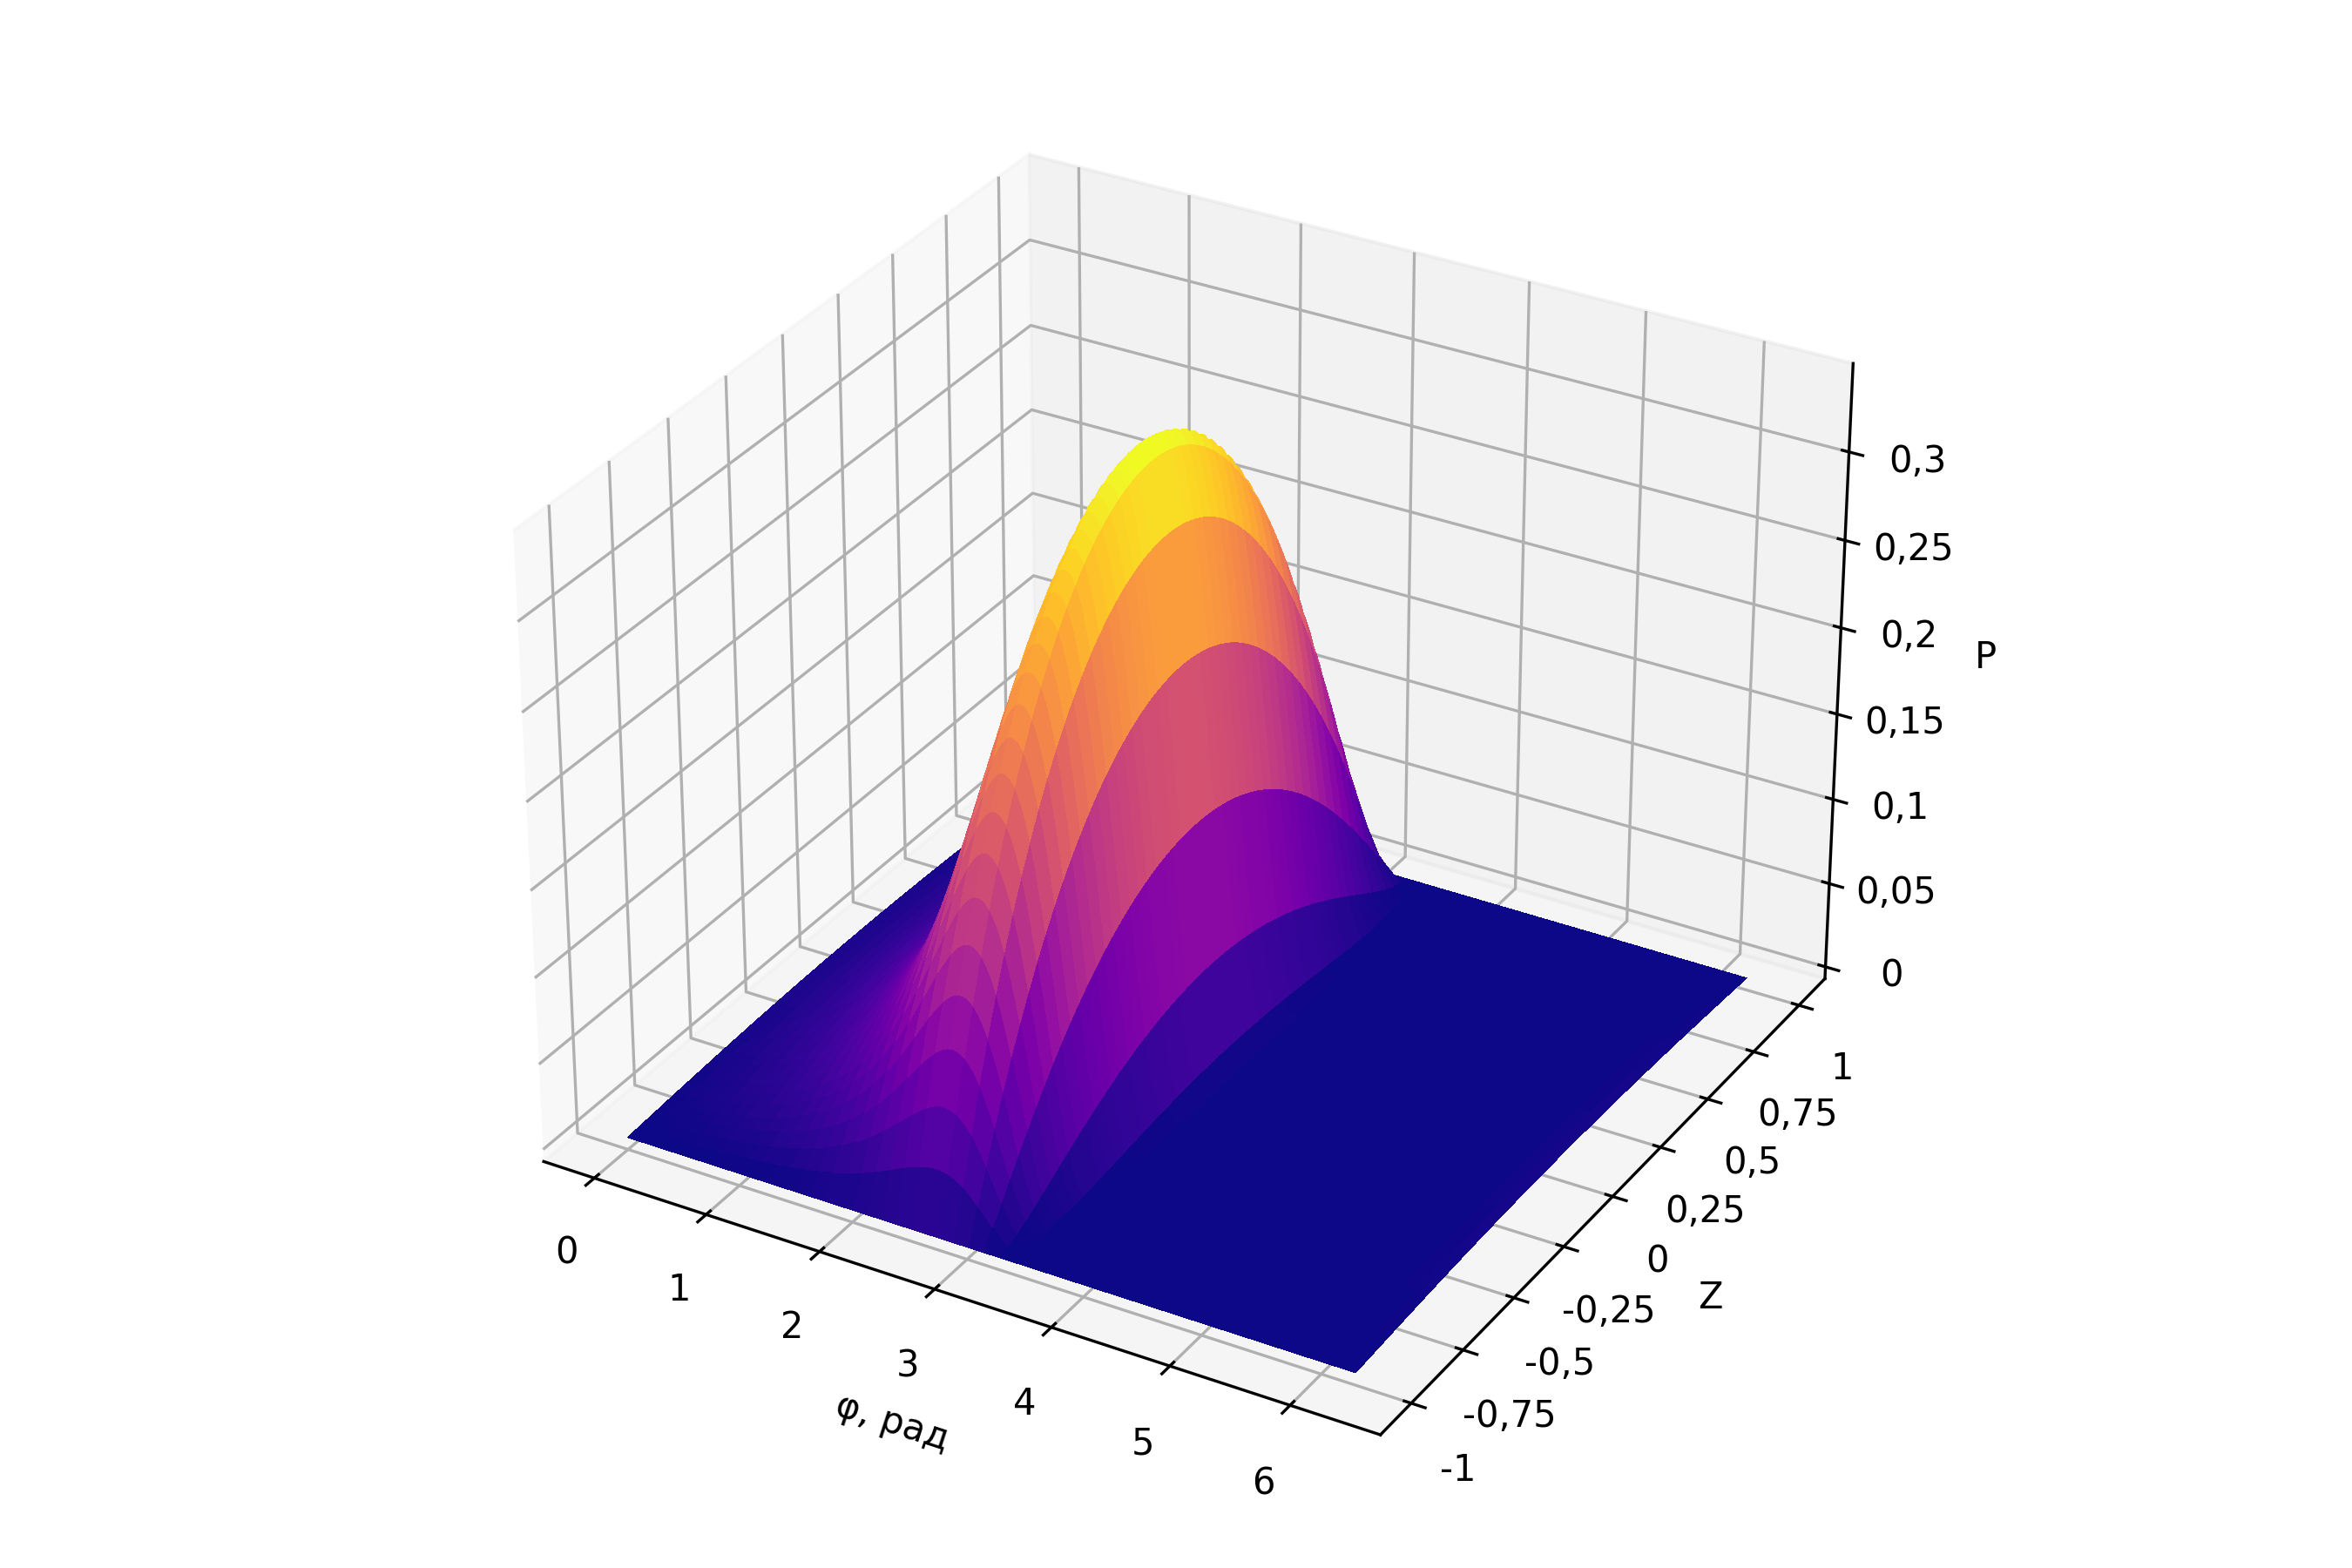
\includegraphics[width=0.75\textwidth]{figures/ch05/fig_5_3.png}
\caption{Поле безразмерного давления $P(\theta, Z)$
  гладкого подшипника при $\varepsilon = 0{,}6$.}
\label{fig:smooth_P3D}
\end{figure}

\begin{figure}[!ht]
\centering
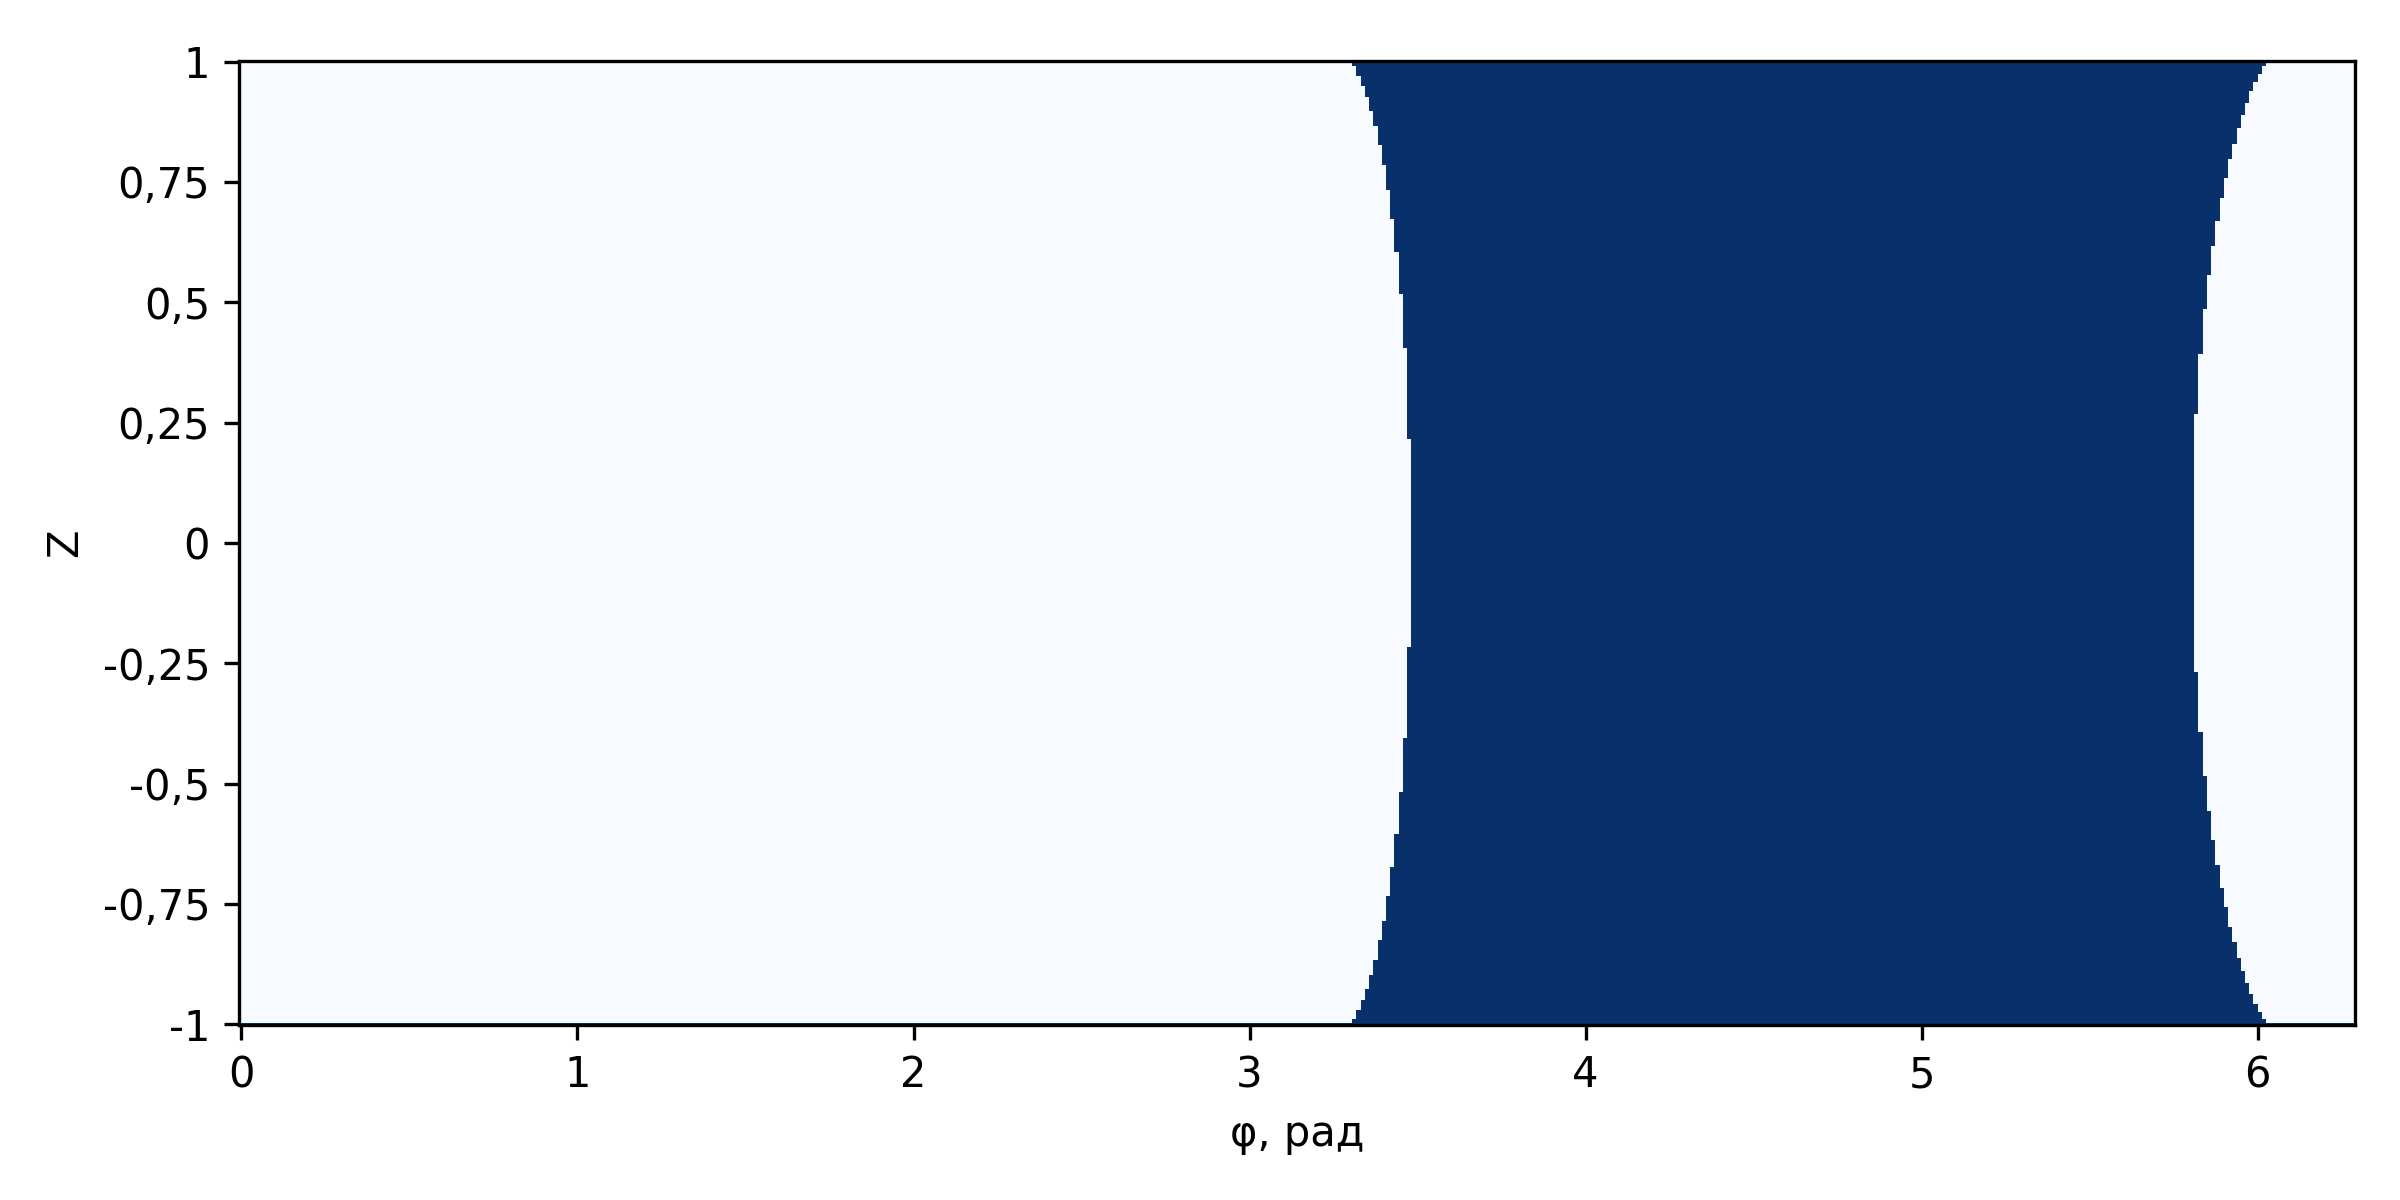
\includegraphics[width=0.75\textwidth]{figures/ch05/fig_5_4.png}
\caption{Карта кавитационной зоны гладкого подшипника
  при $\varepsilon = 0{,}6$. Область $P = 0$ выделена контрастным цветом.}
\label{fig:smooth_cav}
\end{figure}

\FloatBarrier

\textit{Интегральные характеристики.}
По полученному полю давления вычисляются интегральные
характеристики подшипника: компоненты несущей силы
и результирующая сила~$F$ с углом нагружения~$\varphi_{\mathrm{load}}$
(\eqref{eq:func_F_components}, \eqref{eq:func_psi}; в формуле~\eqref{eq:func_psi}
угол в общей постановке обозначен~$\psi$, в настоящей главе используется
обозначение~$\varphi_{\mathrm{load}}$, чтобы не путать с относительным
зазором $\psi = c/R$),
безразмерная сила трения~$f$ и коэффициент трения
$\mu_f = f/F$, а также осевые утечки~$Q_{\mathrm{out}}$
(\eqref{eq:func_Q_journal}). Значения указанных характеристик
при номинальном эксцентриситете приведены в
таблице~\ref{tab:smooth_results}.

\begin{table}[!ht]
\centering
\caption{Интегральные характеристики гладкого подшипника
  при $\varepsilon = \varepsilon_{\mathrm{nom}} = 0{,}6$}
\label{tab:smooth_results}
\begin{tabularx}{\textwidth}{|X|c|c|}
\hline
\multicolumn{1}{|c|}{\textbf{Характеристика}} & \textbf{Обозначение} & \textbf{Значение} \\
\hline
Несущая сила              & $F$, Н                        & 5035{,}7 \\
\hline
Угол нагружения           & $\varphi_{\mathrm{load}}$, $^{\circ}$ & 134{,}1 \\
\hline
Коэффициент трения        & $\mu_f$                       & 0{,}01537 \\
\hline
Осевые утечки             & $Q_{\mathrm{out}}$, мл/с      & 11{,}87 \\
\hline
\end{tabularx}
\end{table}

\FloatBarrier

\textit{Зависимости от эксцентриситета.}
Характерное поведение интегральных характеристик
гидродинамического подшипника при изменении эксцентриситета
определяется нелинейной зависимостью толщины зазора от~$\varepsilon$.
Несущая способность~$F(\varepsilon)$ монотонно возрастает
с ростом эксцентриситета, причём при $\varepsilon \to 1$
рост приобретает резко нелинейный характер, обусловленный
сужением минимального зазора и соответствующим увеличением
пиковых давлений. Коэффициент трения~$\mu_f(\varepsilon)$
убывает с ростом~$\varepsilon$: хотя абсолютные потери на трение
растут из-за повышения вязкого сдвига в зоне минимального зазора,
несущая способность растёт быстрее, и отношение~$\mu_f = f/F$
уменьшается. Осевые утечки~$Q_{\mathrm{out}}(\varepsilon)$
возрастают с ростом~$\varepsilon$: увеличение эксцентриситета
усиливает перепад давления в осевом направлении и расширяет зону
с ненулевым давлением, что приводит к росту осевого потока через
торцы подшипника. Указанные тенденции являются типичными
для гидродинамических подшипников и подтверждаются классическими
результатами. Графики зависимостей~$F(\varepsilon)$,
$\mu_f(\varepsilon)$ и~$Q_{\mathrm{out}}(\varepsilon)$ представлены
на рисунках~\ref{fig:F_vs_epsilon}, \ref{fig:mu_vs_epsilon},
\ref{fig:Q_vs_epsilon}.

\begin{figure}[!ht]
\centering
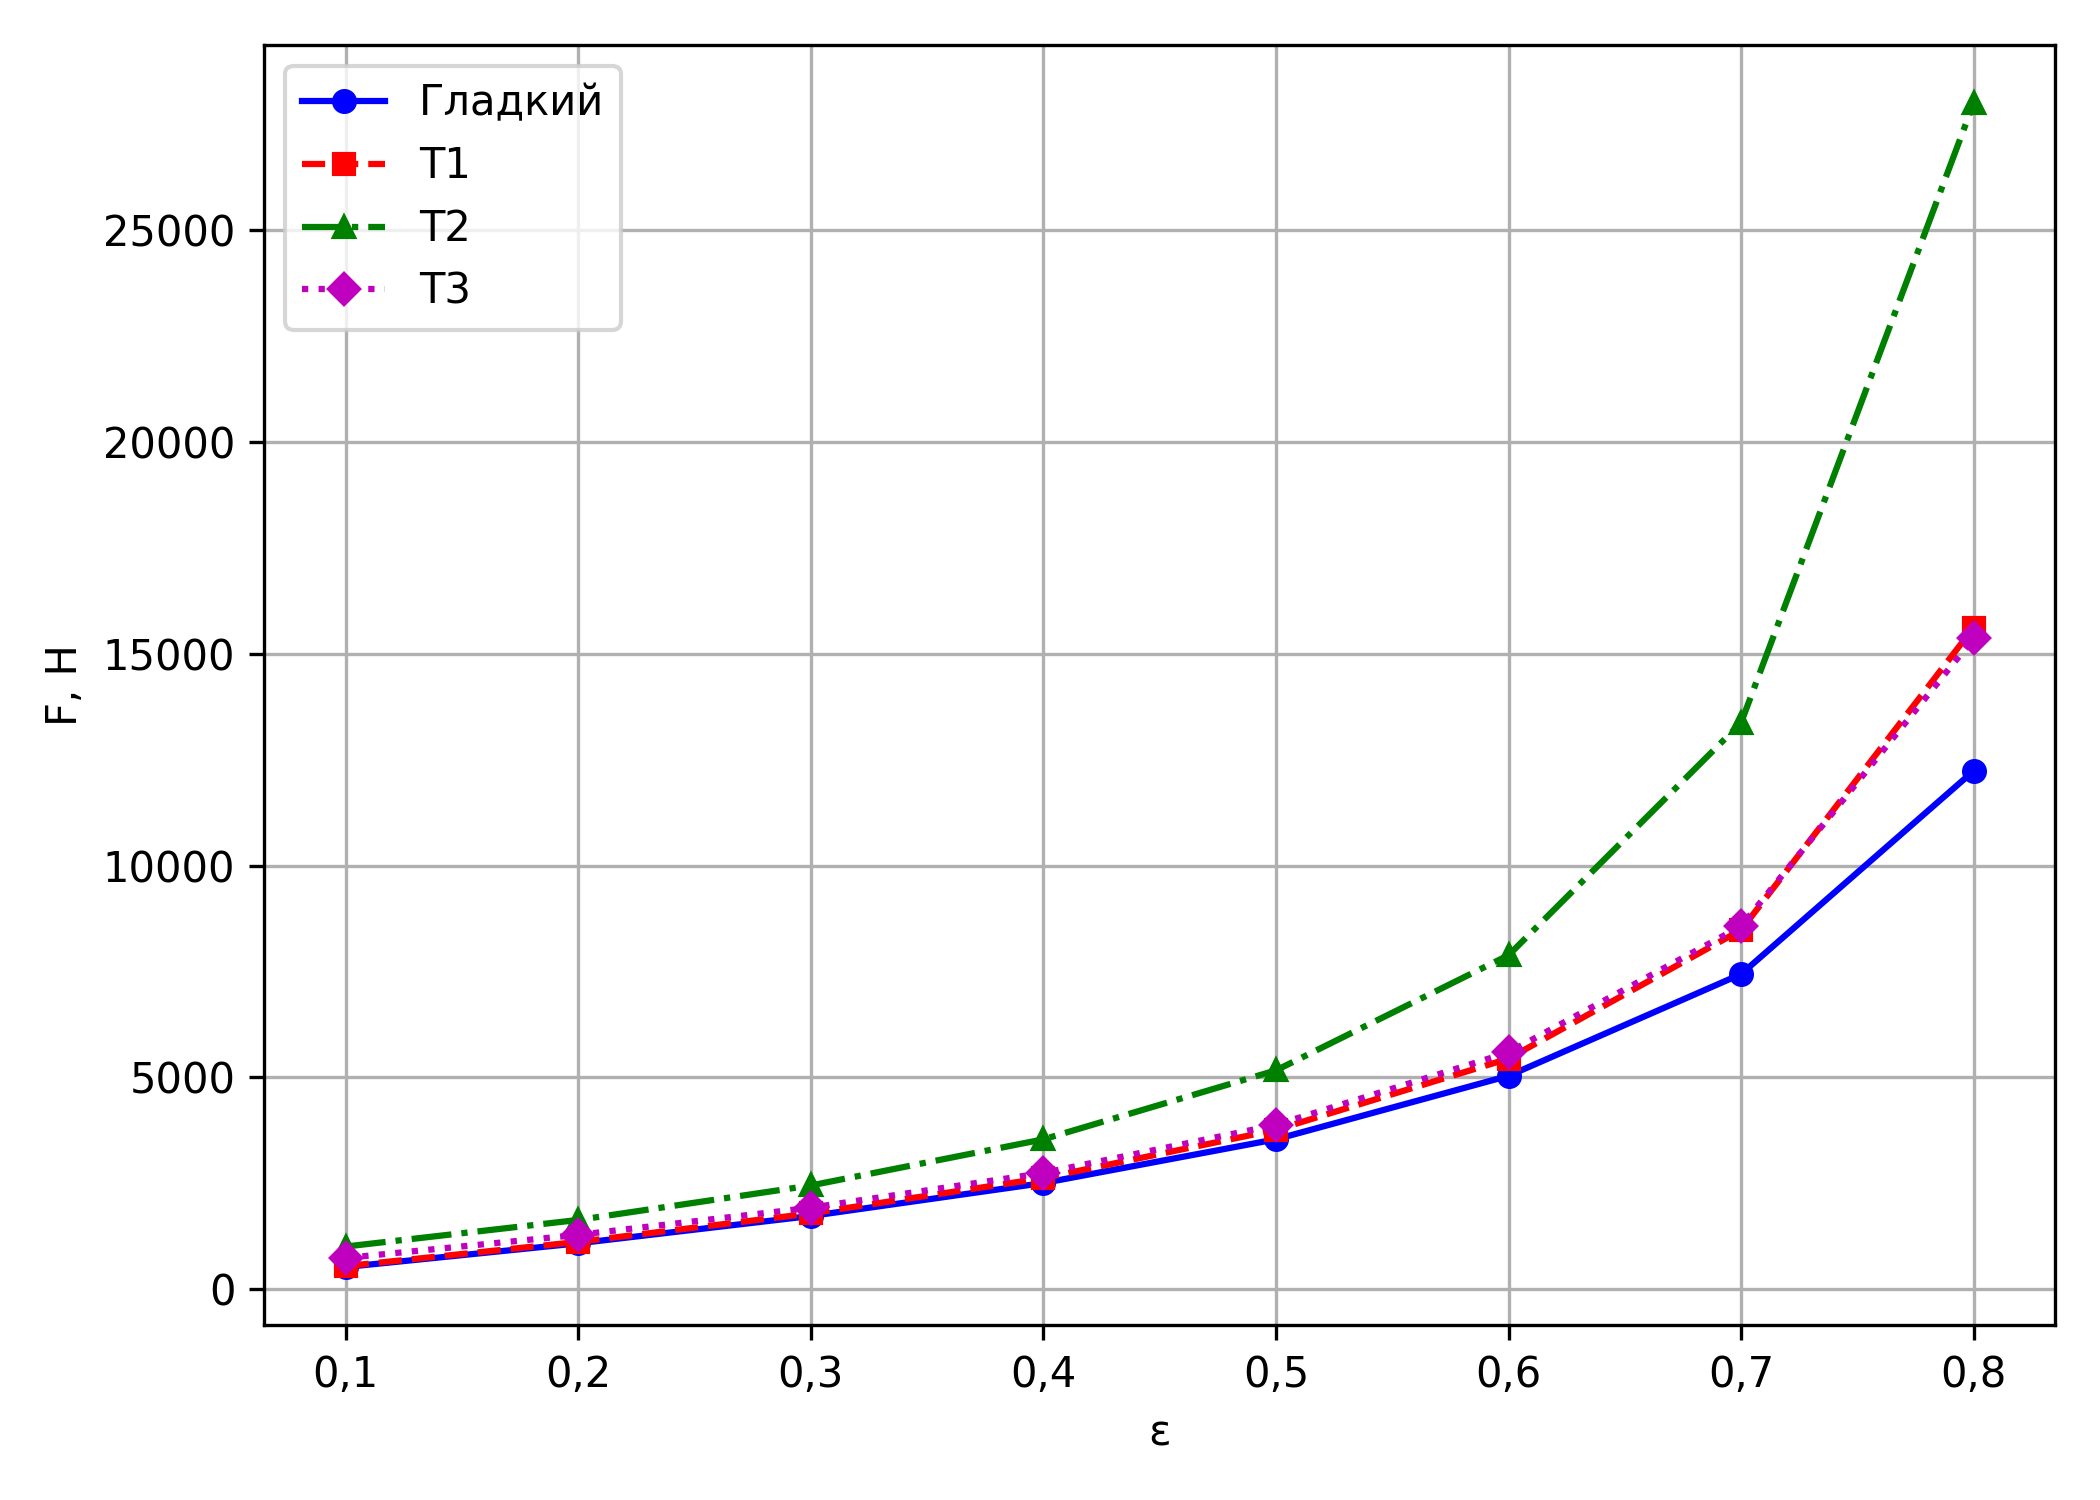
\includegraphics[width=0.75\textwidth]{figures/ch05/fig_5_5.png}
\caption{Зависимость несущей силы~$F$ от эксцентриситета~$\varepsilon$
  для гладкого подшипника и трёх конфигураций текстуры T1, T2, T3.}
\label{fig:F_vs_epsilon}
\end{figure}

\begin{figure}[!ht]
\centering
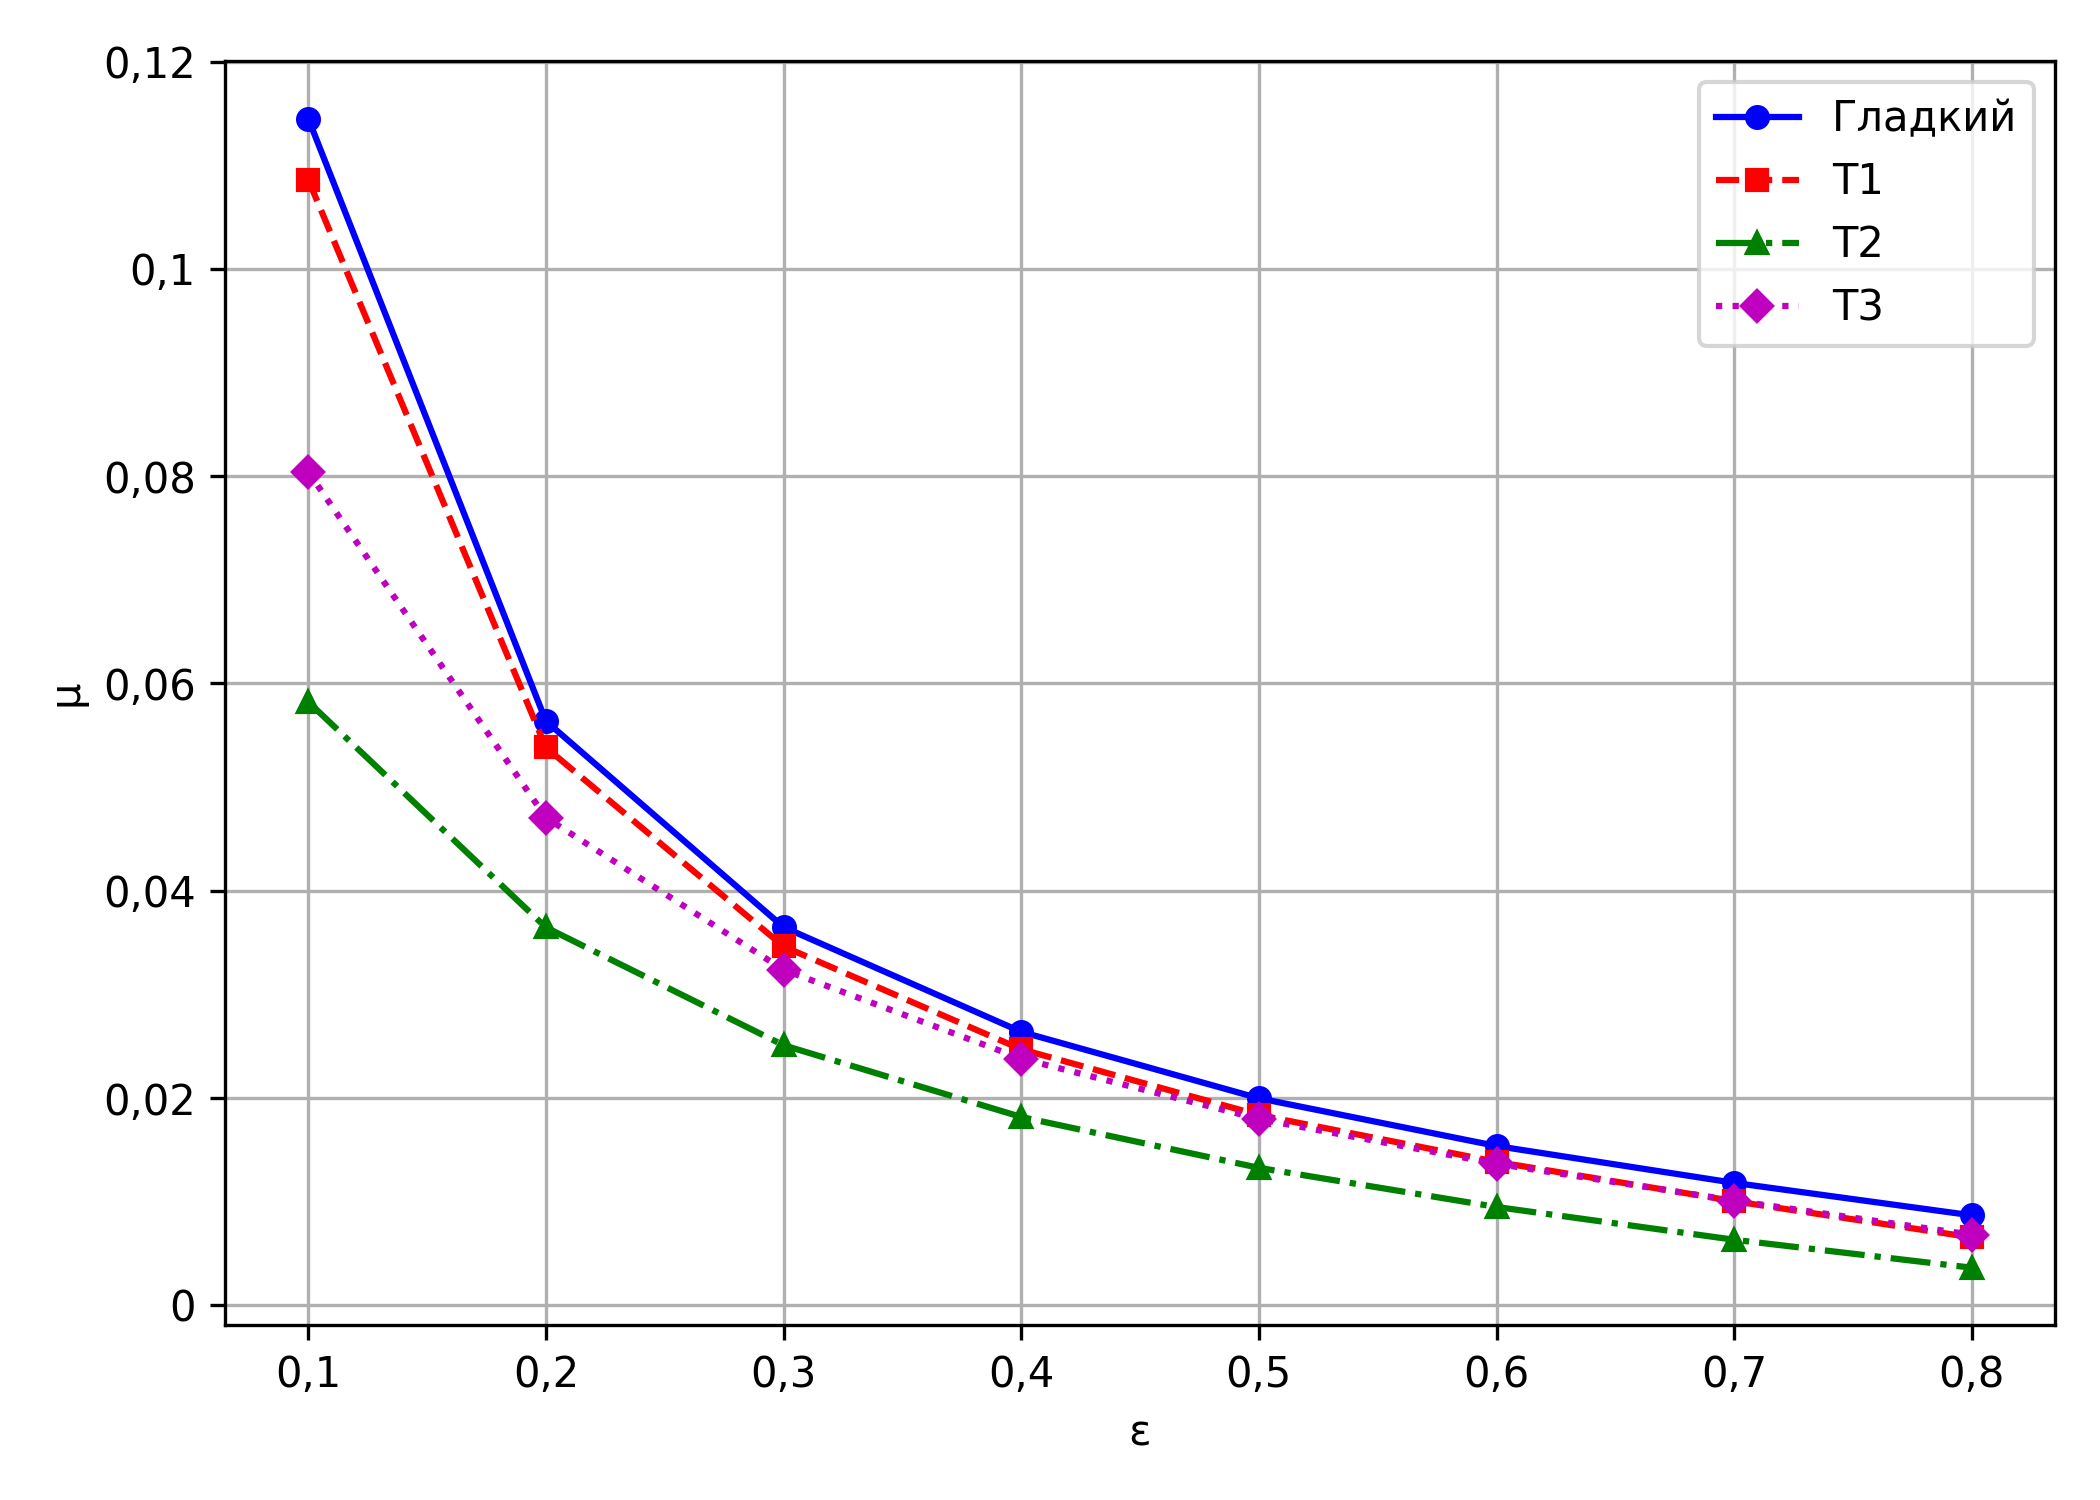
\includegraphics[width=0.75\textwidth]{figures/ch05/fig_5_6.png}
\caption{Зависимость коэффициента трения~$\mu_f$ от эксцентриситета~$\varepsilon$.}
\label{fig:mu_vs_epsilon}
\end{figure}

\begin{figure}[!htbp]
\centering
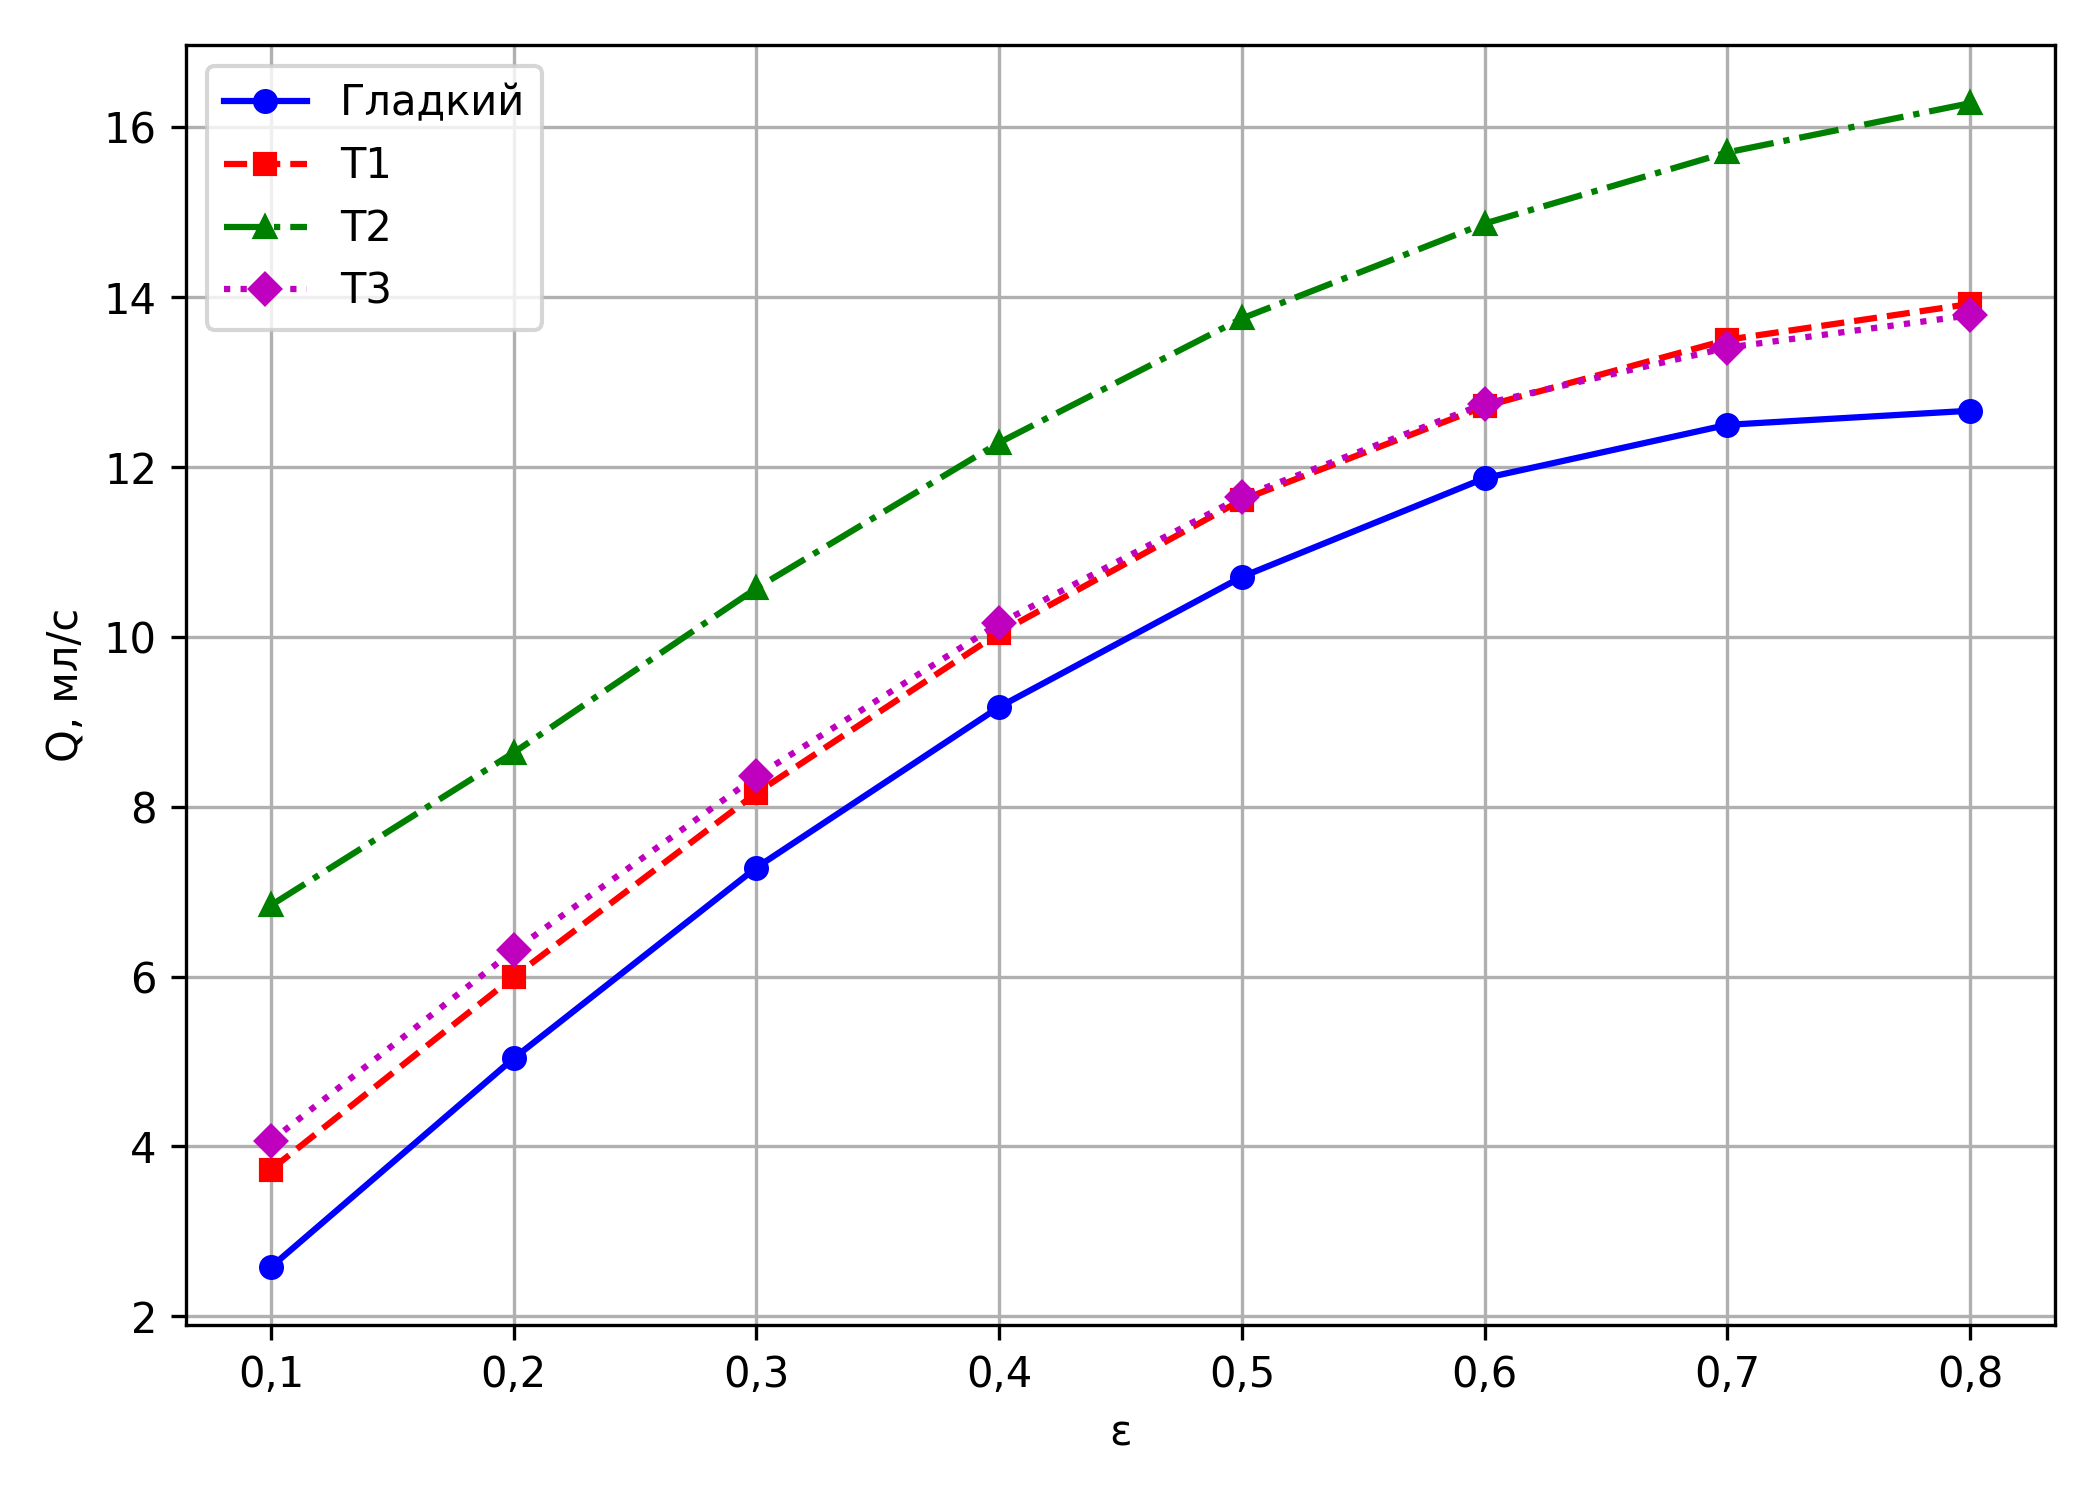
\includegraphics[width=0.75\textwidth]{figures/ch05/fig_5_7.png}
\caption{Зависимость осевых утечек~$Q_{\mathrm{out}}$ от эксцентриситета~$\varepsilon$.}
\label{fig:Q_vs_epsilon}
\end{figure}

\FloatBarrier

Полученные результаты для гладкого подшипника служат эталоном,
относительно которого оценивается влияние детерминированных
микроструктур в последующих разделах.

\section{Выбор и параметры микроструктуры}

В качестве элементов микрорельефа выбраны эллипсоидальные лунки
с профилем~\eqref{eq:profile_ellipsoidal}, представляющие
наиболее распространённый тип текстуры в задачах
гидродинамической смазки. Раскладка элементов выполнена
по шахматной схеме~\eqref{eq:layout_staggered}, обеспечивающей
равномерное заполнение текстурированной зоны при заданном
коэффициенте покрытия.

Выбор зоны нанесения микроструктур определяется физическим
механизмом их воздействия на поле давления. В радиальном
подшипнике текстурирование может охватывать всю поверхность
вкладыша, только зону сходящегося клина, зону максимального
давления или зону расходящегося клина. Расположение текстурированной
области относительно зоны давления существенно влияет на результат:
лунки в области сходящегося зазора способны усилить
гидродинамический эффект, тогда как лунки в зоне расходящегося
зазора могут расширить кавитационную область.

Безразмерные параметры текстуры определены в подразделе~2.2.4:
глубина элемента~$H_p$~\eqref{eq:Hp_nondim}, безразмерные
полуоси~$A^*$, $B^*$ и коэффициент покрытия~$\varphi$.
Рассматриваются три конфигурации текстуры, различающиеся
глубиной элементов и зоной нанесения
(таблица~\ref{tab:texture_configs}).

\begin{table}[!ht]
\centering
\caption{Параметры рассматриваемых конфигураций текстуры}
\label{tab:texture_configs}
\begin{tabularx}{\textwidth}{|X|c|c|c|c|c|}
\hline
\multicolumn{1}{|c|}{\textbf{Конфигурация}}   & $\boldsymbol{H_p}$ & $\boldsymbol{A^*}$ & $\boldsymbol{B^*}$   & $\boldsymbol{\varphi}$ & \textbf{Зона нанесения} \\
\hline
T1 & 0{,}20 & 0{,}0861 & 0{,}0633 & 0{,}240 & $90^{\circ}$--$270^{\circ}$ \\
\hline
T2 & 0{,}40 & 0{,}0861 & 0{,}0633 & 0{,}240 & $90^{\circ}$--$270^{\circ}$ \\
\hline
T3 & 0{,}20 & 0{,}0861 & 0{,}0633 & 0{,}240 & $0^{\circ}$--$180^{\circ}$ \\
\hline
\end{tabularx}
\end{table}

\FloatBarrier

Конфигурации T1 и T2 различаются глубиной лунок: T2 имеет вдвое
большую глубину ($H_p = 0{,}40$) при той же зоне нанесения
($90^{\circ}$--$270^{\circ}$). Сектор $90^{\circ}$--$270^{\circ}$
включает область минимального зазора ($\theta \approx \pi$)
и часть расходящегося участка. Конфигурация T3 отличается зоной
нанесения: лунки расположены в секторе $0^{\circ}$--$180^{\circ}$
(зона сходящегося клина) при глубине, совпадающей с T1.

Карта кавитационной зоны для конфигурации~T1, на которой различима
шахматная раскладка элементов, представлена на
рисунке~\ref{fig:texture_layout}.

\begin{figure}[!ht]
\centering
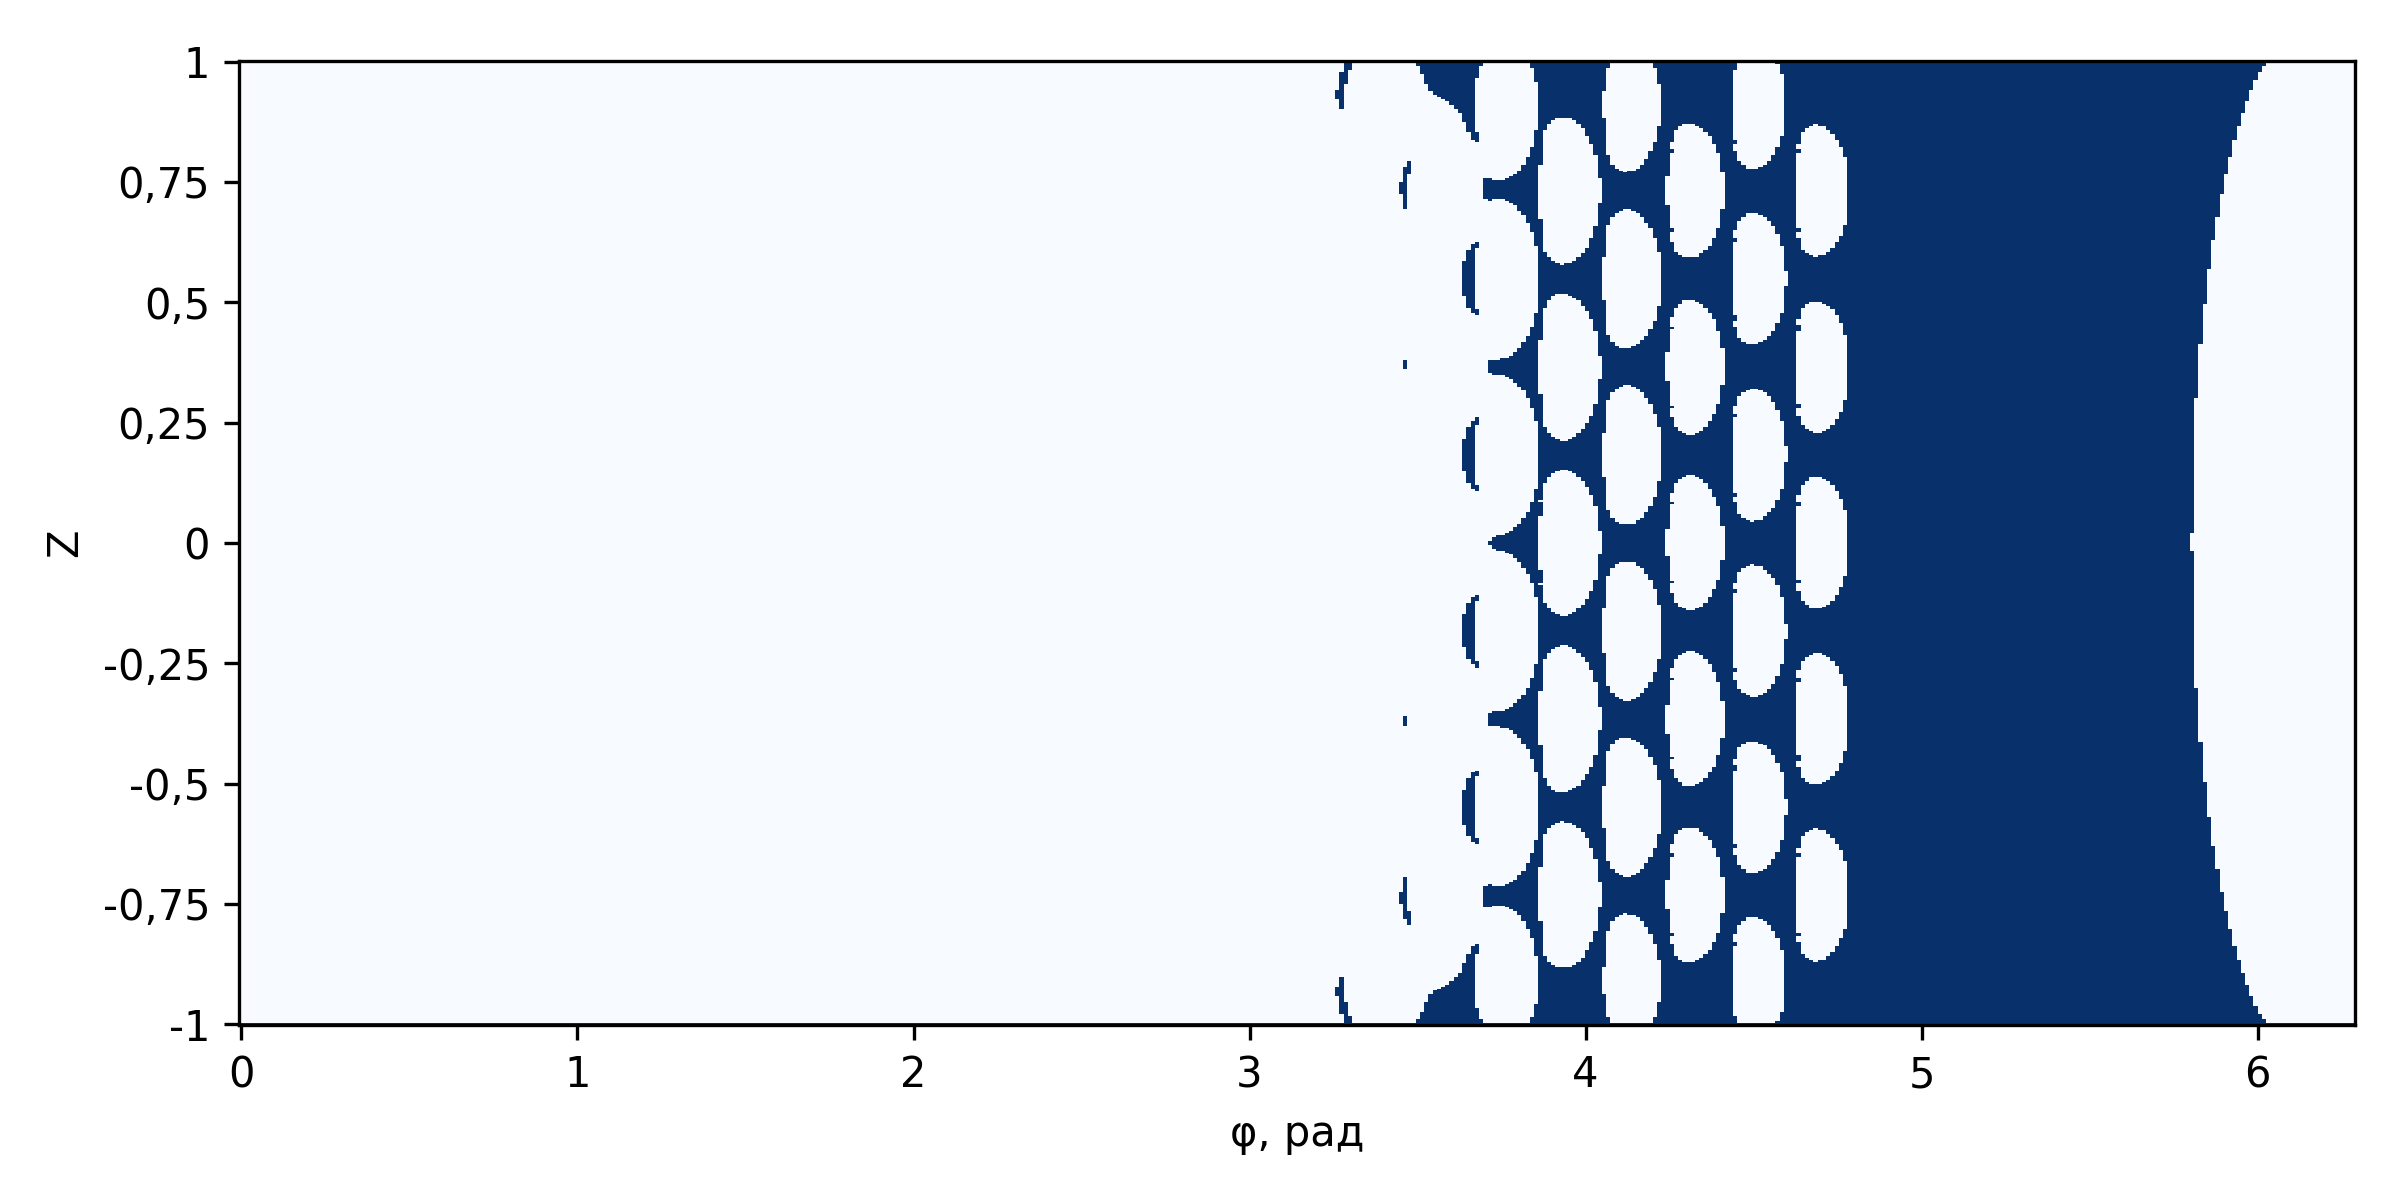
\includegraphics[width=0.75\textwidth]{figures/ch05/fig_5_8.png}
\caption{Карта кавитационной зоны текстурированного подшипника (конфигурация~T1,
  $\varepsilon = 0{,}6$). Шахматная раскладка элементов различима
  по локальным <<островкам>> зоны $P > 0$ внутри лунок.}
\label{fig:texture_layout}
\end{figure}


\section{Сравнение гладкого и текстурированного подшипников}

\textit{Физический механизм влияния микроструктур.}
Эллипсоидальные лунки, нанесённые на рабочую поверхность
вкладыша, создают локальные расширения и сужения зазора,
формируя дополнительные микроклинья. В зоне сходящегося
зазора подшипника, где давление формируется за счёт
макроскопического клинового эффекта~\eqref{eq:journal_h_ch5},
лунки создают дополнительные локальные области конвергенции,
что может усилить генерацию давления и повысить несущую
способность. В расходящейся зоне, где давление снижается
до уровня кавитации, лунки способны расширить кавитационную
область, изменяя баланс потоков на границе фазового перехода.
Результирующее влияние микроструктур на интегральные
характеристики определяется совокупностью этих эффектов
и зависит от зоны нанесения, глубины и коэффициента покрытия~$\varphi$.

\textit{Нормированные показатели эффективности.}
Для количественного сравнения текстурированного
и гладкого подшипников вводятся нормированные показатели:
\begin{equation}
\begin{split}
  &G_F = \frac{F_{\mathrm{tex}}}{F_{\mathrm{smooth}}}, \quad
  G_f = \frac{\mu_{f,\mathrm{tex}}}{\mu_{f,\mathrm{smooth}}}, \\
  &G_Q = \frac{Q_{\mathrm{out,tex}}}{Q_{\mathrm{out,smooth}}}, \quad
  G_h = \frac{h_{\min,\mathrm{tex}}}{h_{\min,\mathrm{smooth}}}.
\end{split}
  \label{eq:gain_factors}
\end{equation}
Значение~$G > 1$ указывает на рост соответствующего показателя
при текстурировании, $G < 1$~-- на снижение. С точки зрения
эксплуатации желательны~$G_F > 1$ (рост несущей способности),
$G_f < 1$ (снижение трения) и $G_h > 1$ (увеличение минимального
зазора, повышение запаса по толщине плёнки).

\textit{Интегральные характеристики при номинальном эксцентриситете.}
Результаты расчёта для гладкого подшипника и трёх конфигураций
текстуры при $\varepsilon = 0{,}6$ сведены в
таблицу~\ref{tab:comparison_results}.

\begin{table}[!ht]
\centering
\caption{Интегральные характеристики подшипников при $\varepsilon = 0{,}6$}
\label{tab:comparison_results}
\resizebox{\textwidth}{!}{%
\begin{tabular}{|l|c|c|c|c|c|c|c|c|}
\hline
\multicolumn{1}{|c|}{\textbf{Вариант}} & $\boldsymbol{F}$, \textbf{Н} & $\boldsymbol{\varphi_{\mathrm{load}}}$, $\boldsymbol{^{\circ}}$ & $\boldsymbol{\mu_f}$ & $\boldsymbol{Q_{\mathrm{out}}}$, \textbf{мл/с} & $\boldsymbol{G_F}$ & $\boldsymbol{G_f}$ & $\boldsymbol{G_Q}$ & $\boldsymbol{G_h}$ \\
\hline
Гладкий & 5035{,}7 & 134{,}1 & 0{,}01537 & 11{,}87 & --- & --- & --- & --- \\
\hline
T1 & 5443{,}2 & 139{,}3 & 0{,}01384 & 12{,}72 & 1{,}081 & 0{,}900 & 1{,}071 & 1{,}00 \\
\hline
T2 & 7884{,}5 & 150{,}3 & 0{,}00949 & 14{,}87 & 1{,}566 & 0{,}617 & 1{,}253 & 1{,}00 \\
\hline
T3 & 5588{,}9 & 139{,}4 & 0{,}01366 & 12{,}75 & 1{,}110 & 0{,}888 & 1{,}074 & 1{,}00 \\
\hline
\end{tabular}%
}
\end{table}

\FloatBarrier

Конфигурация T2 демонстрирует наибольший прирост несущей
способности ($G_F = 1{,}566$) и наибольшее снижение коэффициента
трения ($G_f = 0{,}617$), однако сопровождается существенным
увеличением осевых утечек ($G_Q = 1{,}253$). Конфигурации T1 и T3
показывают близкие результаты, что свидетельствует о меньшей
чувствительности характеристик к зоне нанесения при умеренной
глубине лунок ($H_p = 0{,}20$).

Показатель $G_h = 1{,}00$ для всех конфигураций означает, что
глобальный минимум толщины плёнки в расчёте достигается вне лунок:
вследствие дискретного покрытия поверхности $\min H(\theta,Z)
= 1 - \varepsilon$, и минимальный зазор определяется исключительно
эксцентриситетом.

Нормированные показатели эффективности для трёх конфигураций
наглядно сопоставлены на рисунке~\ref{fig:gains_nom}.

\textit{Поля давления и кавитация.}
Текстурирование поверхности вкладыша модифицирует распределение
давления в смазочном слое. В области расположения лунок поле
давления приобретает локальные возмущения~-- каждый элемент
микрорельефа формирует собственный микроклин, вносящий вклад
в интегральный баланс. Одновременно изменяется конфигурация
кавитационной области: распределение зон $P = 0$ и их суммарная
площадь зависят от параметров текстуры. Сопоставление
полей давления и карт кавитации для гладкого
и текстурированного подшипников при одинаковом значении
эксцентриситета представлено на
рисунках~\ref{fig:P3D_T1}, \ref{fig:texture_layout}, \ref{fig:P3D_T2}, \ref{fig:cav_T2}, \ref{fig:P3D_T3}, \ref{fig:cav_T3}.

\begin{figure}[!ht]
\centering
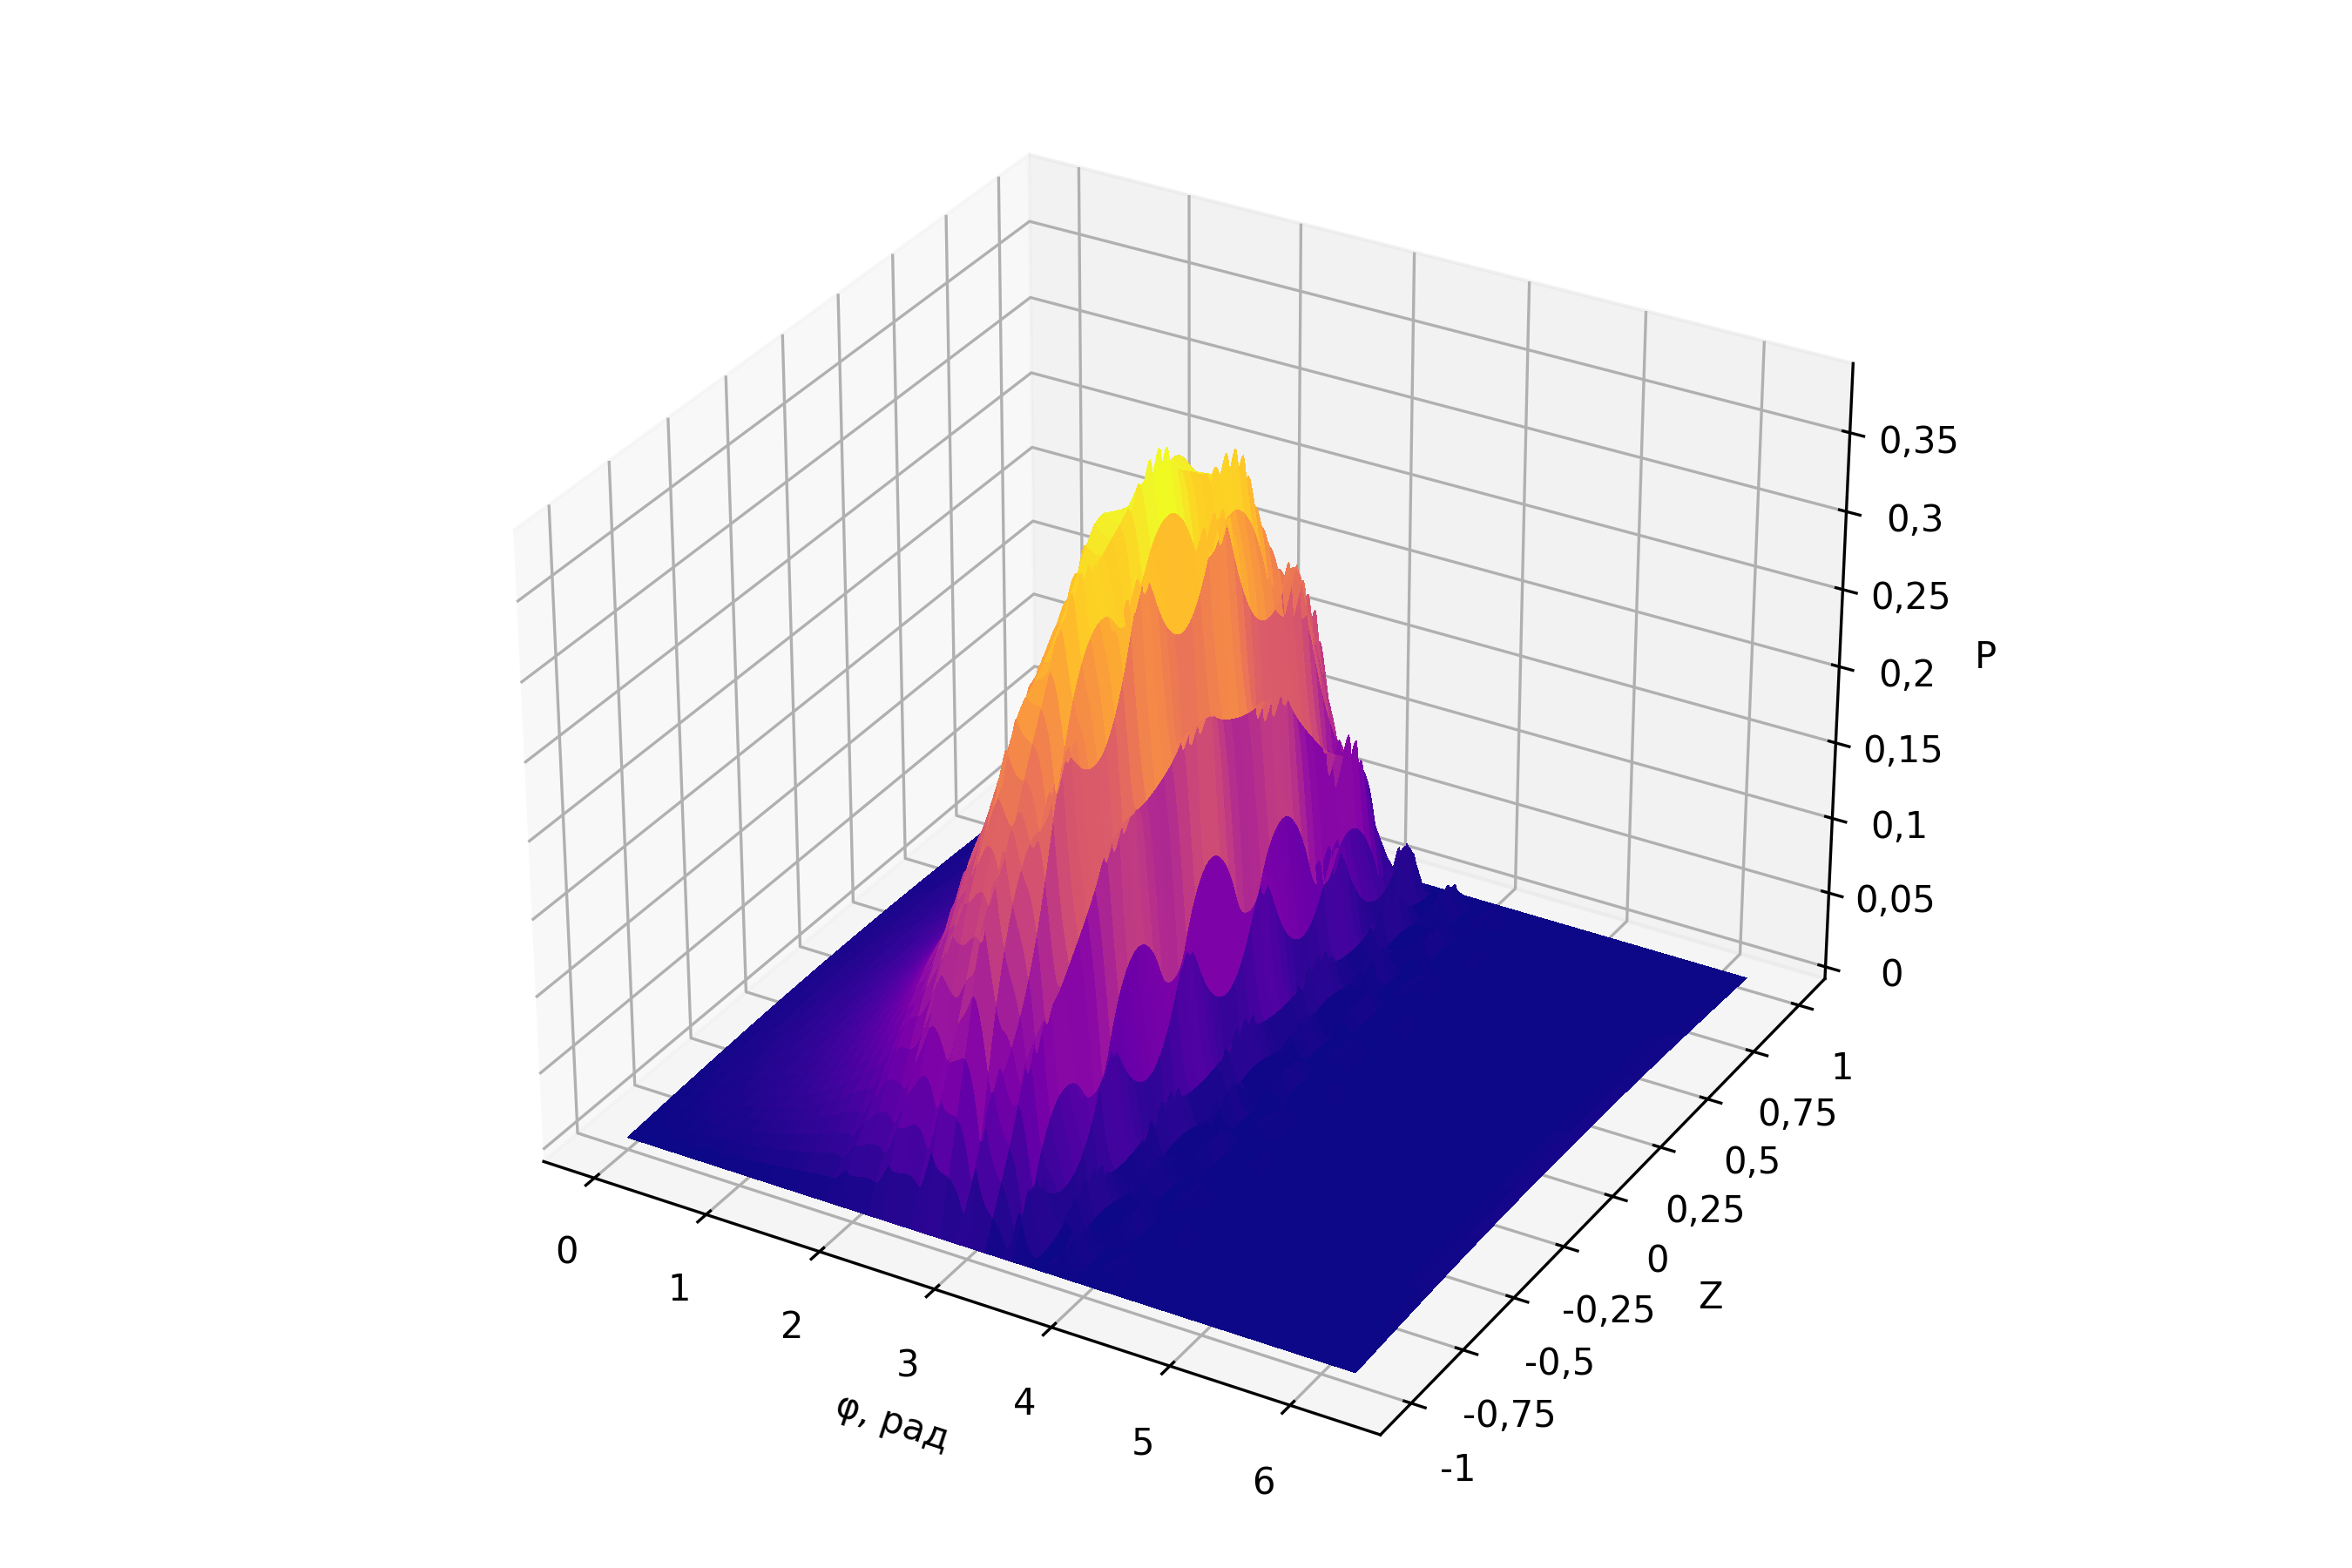
\includegraphics[width=0.75\textwidth]{figures/ch05/fig_5_9.png}
\caption{Поле давления $P(\theta, Z)$ для конфигурации~T1
  ($H_p = 0{,}20$, зона $90^{\circ}$--$270^{\circ}$)
  при $\varepsilon = 0{,}6$.}
\label{fig:P3D_T1}
\end{figure}


\begin{figure}[!ht]
\centering
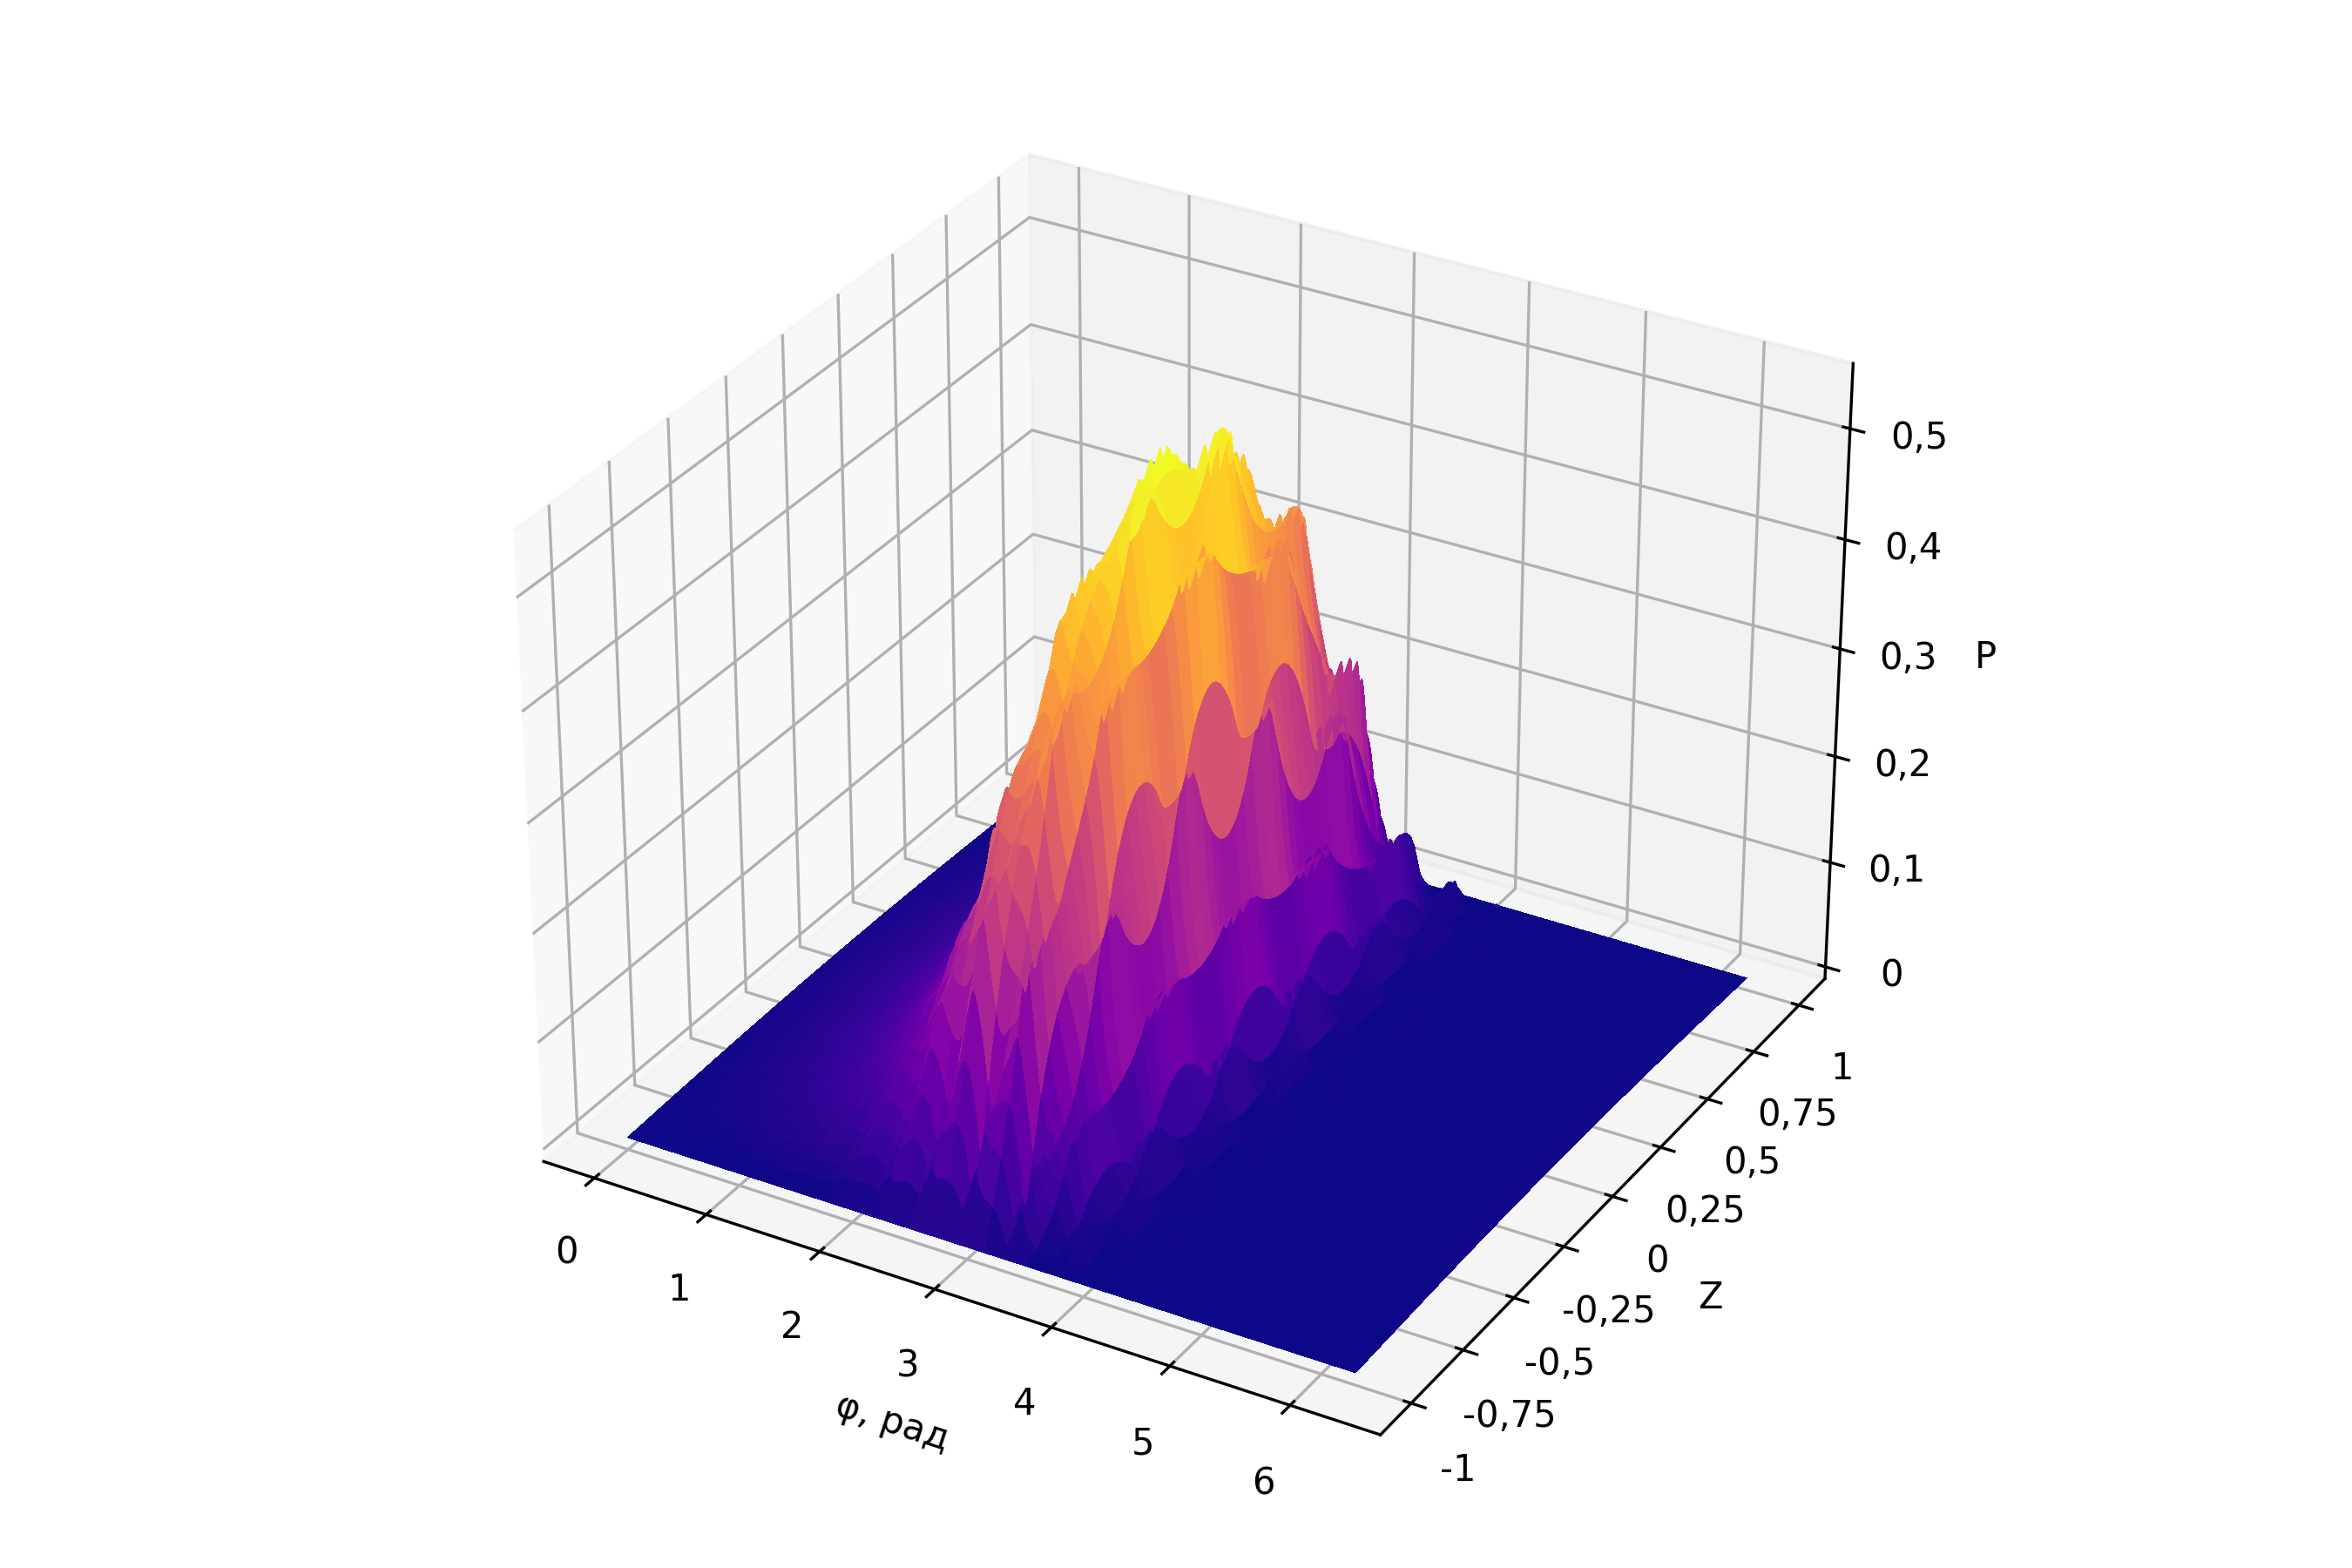
\includegraphics[width=0.75\textwidth]{figures/ch05/fig_5_10.png}
\caption{Поле давления $P(\theta, Z)$ для конфигурации~T2
  ($H_p = 0{,}40$, зона $90^{\circ}$--$270^{\circ}$)
  при $\varepsilon = 0{,}6$. Увеличение глубины лунок приводит
  к более выраженной ряби на поверхности давления.}
\label{fig:P3D_T2}
\end{figure}

\begin{figure}[!ht]
\centering
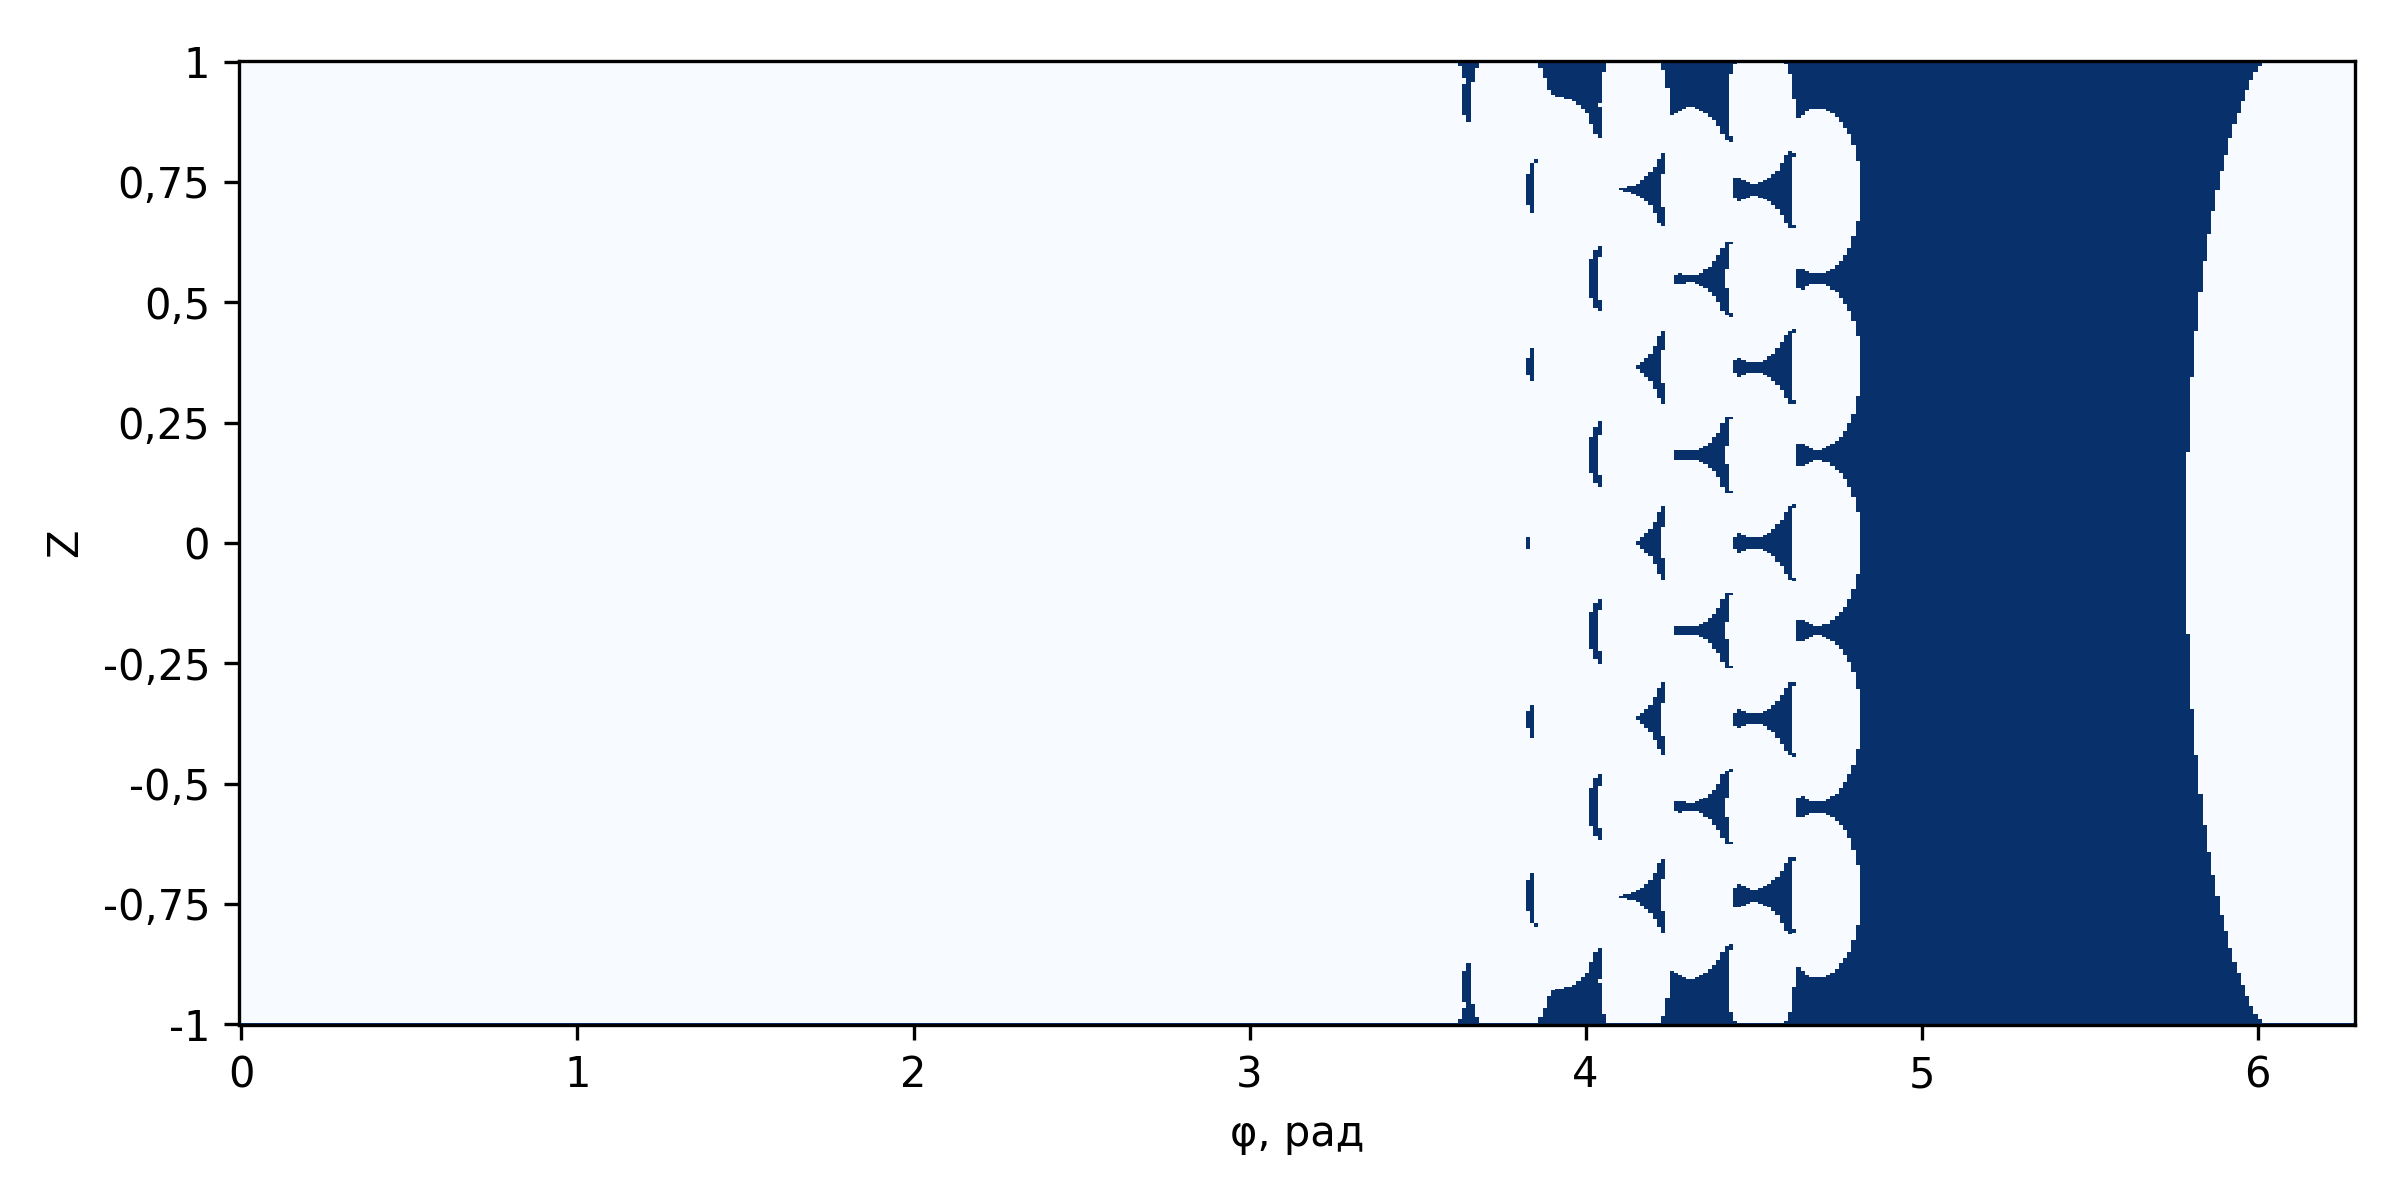
\includegraphics[width=0.75\textwidth]{figures/ch05/fig_5_11.png}
\caption{Карта кавитационной зоны для конфигурации~T2
  ($H_p = 0{,}40$, зона $90^{\circ}$--$270^{\circ}$)
  при $\varepsilon = 0{,}6$.}
\label{fig:cav_T2}
\end{figure}

\begin{figure}[!ht]
\centering
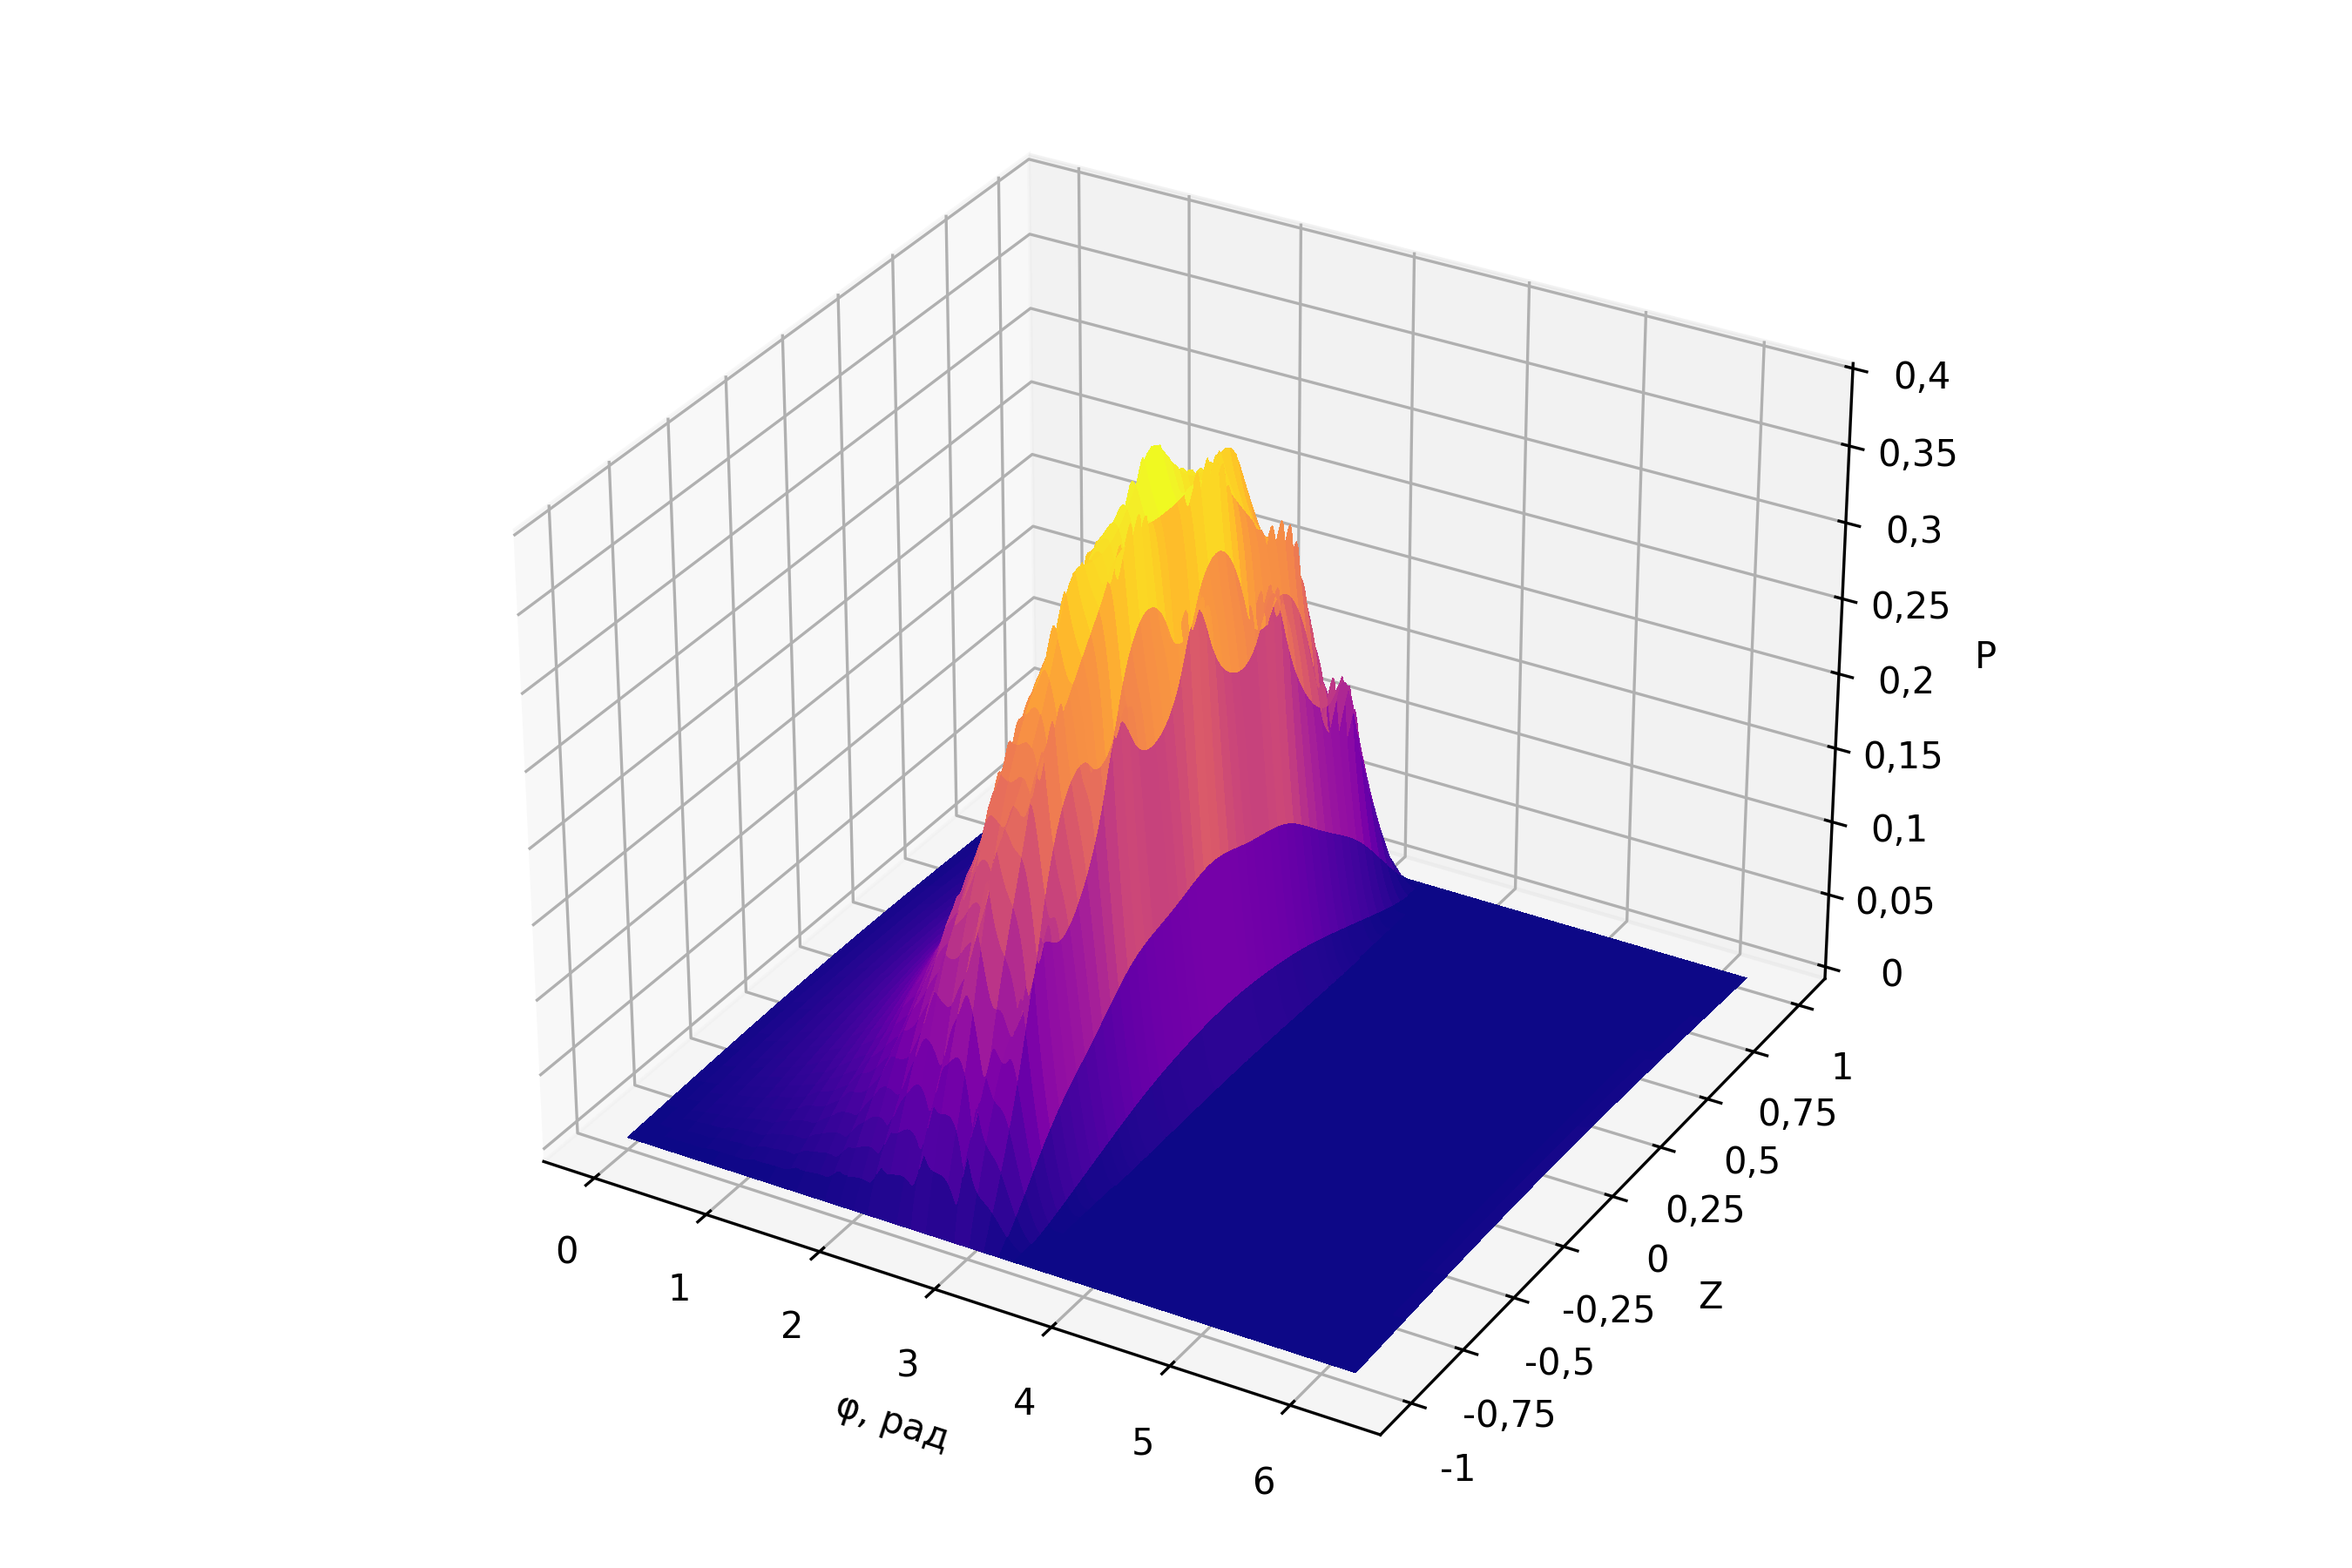
\includegraphics[width=0.75\textwidth]{figures/ch05/fig_5_12.png}
\caption{Поле давления $P(\theta, Z)$ для конфигурации~T3
  ($H_p = 0{,}20$, зона $0^{\circ}$--$180^{\circ}$)
  при $\varepsilon = 0{,}6$. Перенос текстурированной зоны
  в область сходящегося клина изменяет характер локальных возмущений.}
\label{fig:P3D_T3}
\end{figure}

\begin{figure}[!ht]
\centering
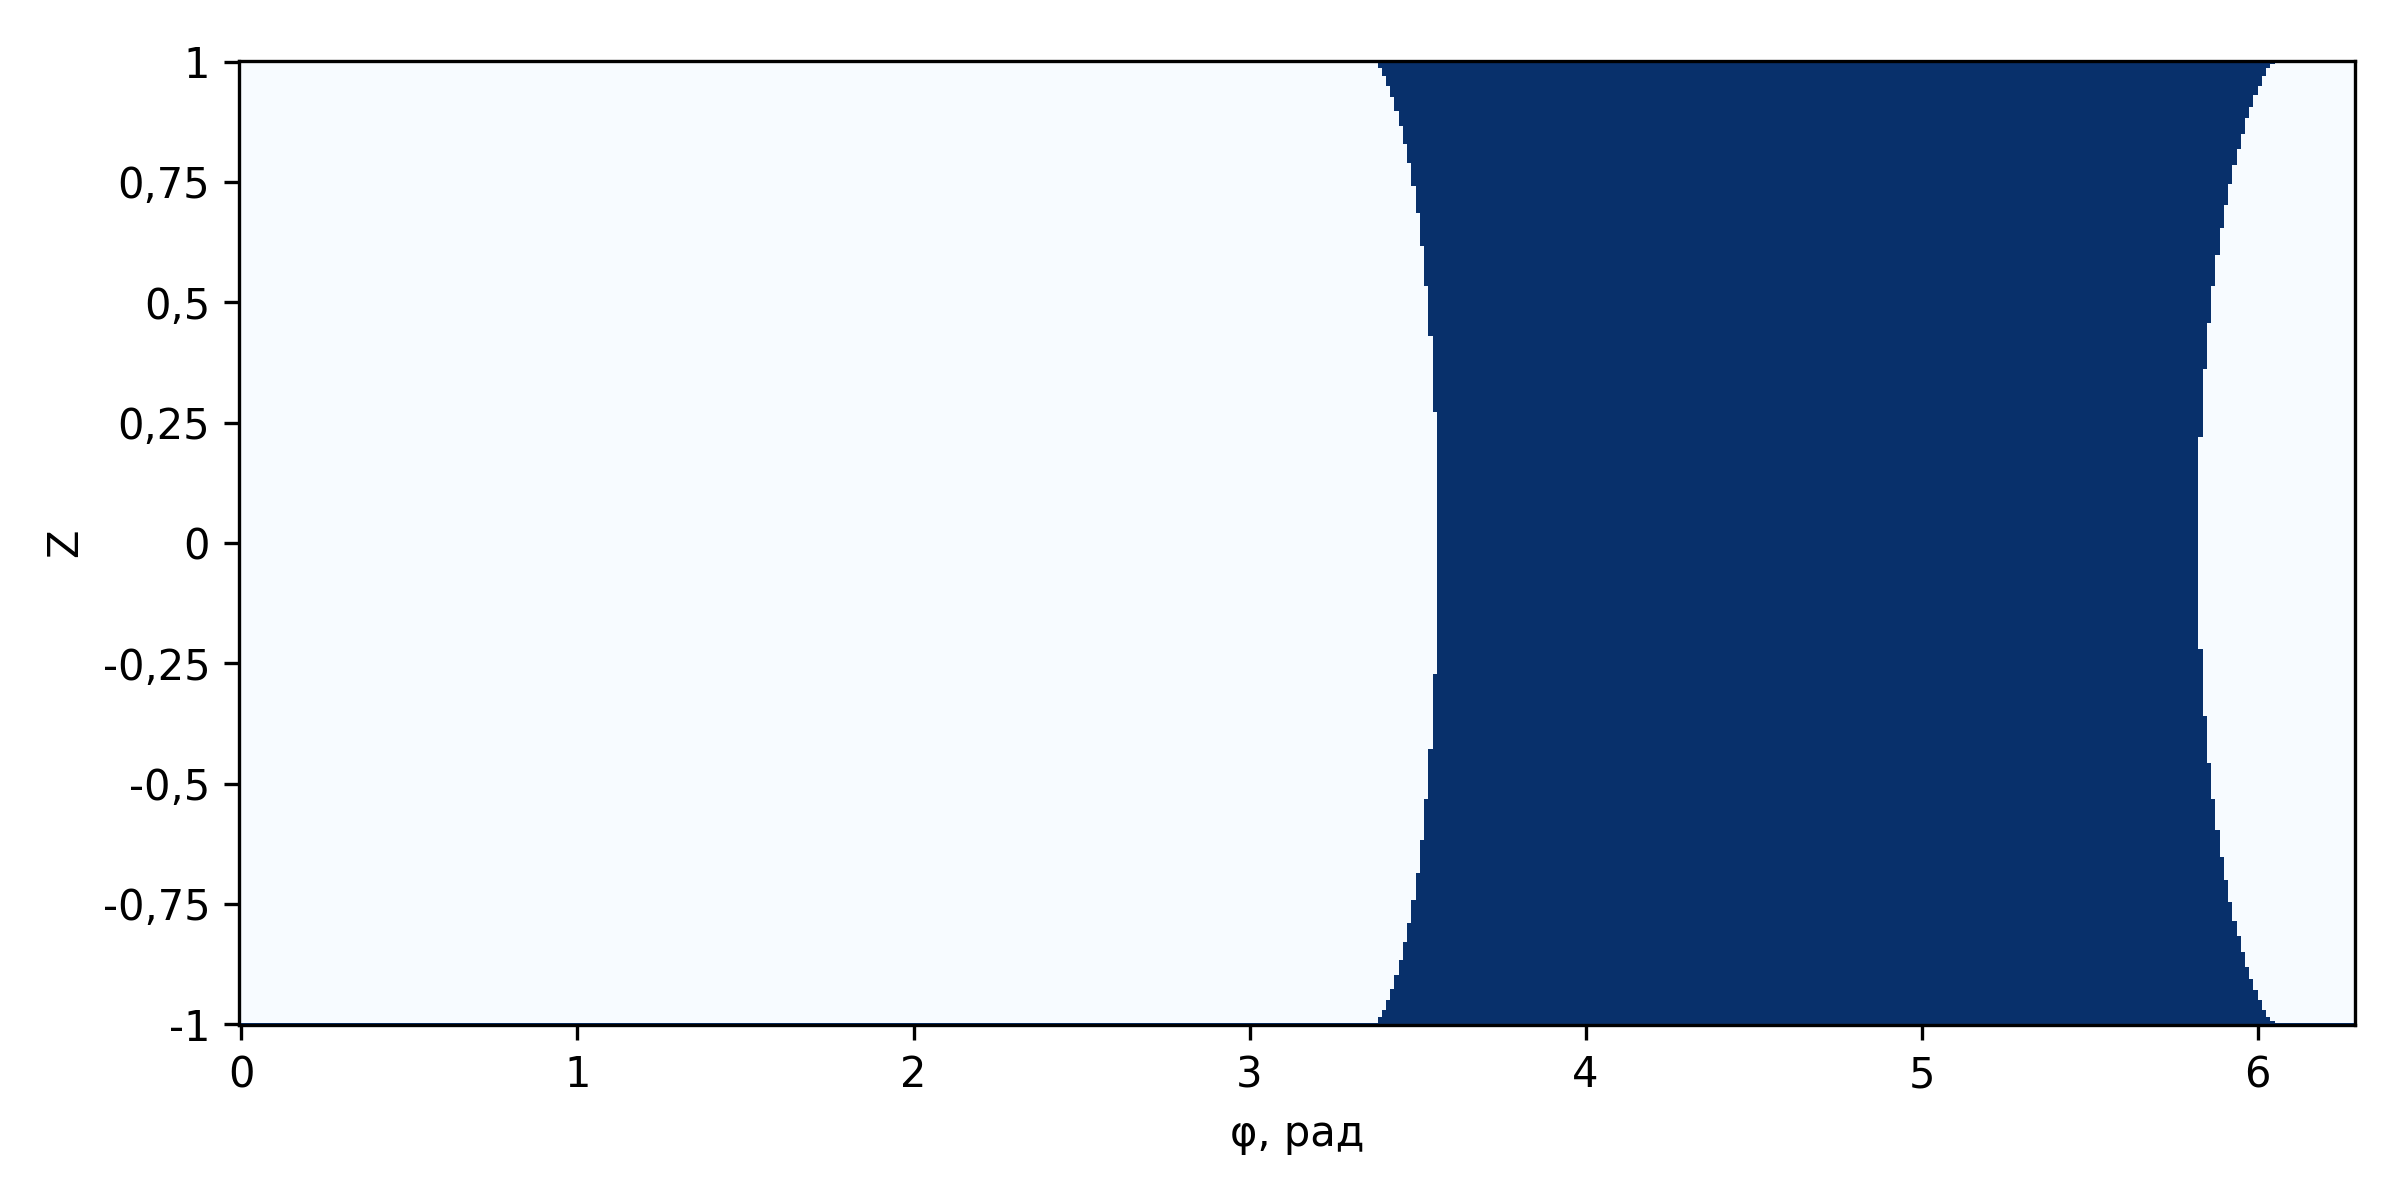
\includegraphics[width=0.75\textwidth]{figures/ch05/fig_5_13.png}
\caption{Карта кавитационной зоны для конфигурации~T3
  ($H_p = 0{,}20$, зона $0^{\circ}$--$180^{\circ}$)
  при $\varepsilon = 0{,}6$.}
\label{fig:cav_T3}
\end{figure}

\FloatBarrier

\textit{Распределение давления в среднем сечении.}
Для более детального анализа на рисунке~\ref{fig:comparison_curves}
представлено распределение давления $P(\theta)$ при $Z = 0$
для гладкого подшипника и конфигурации~T1.

\begin{figure}[!ht]
\centering
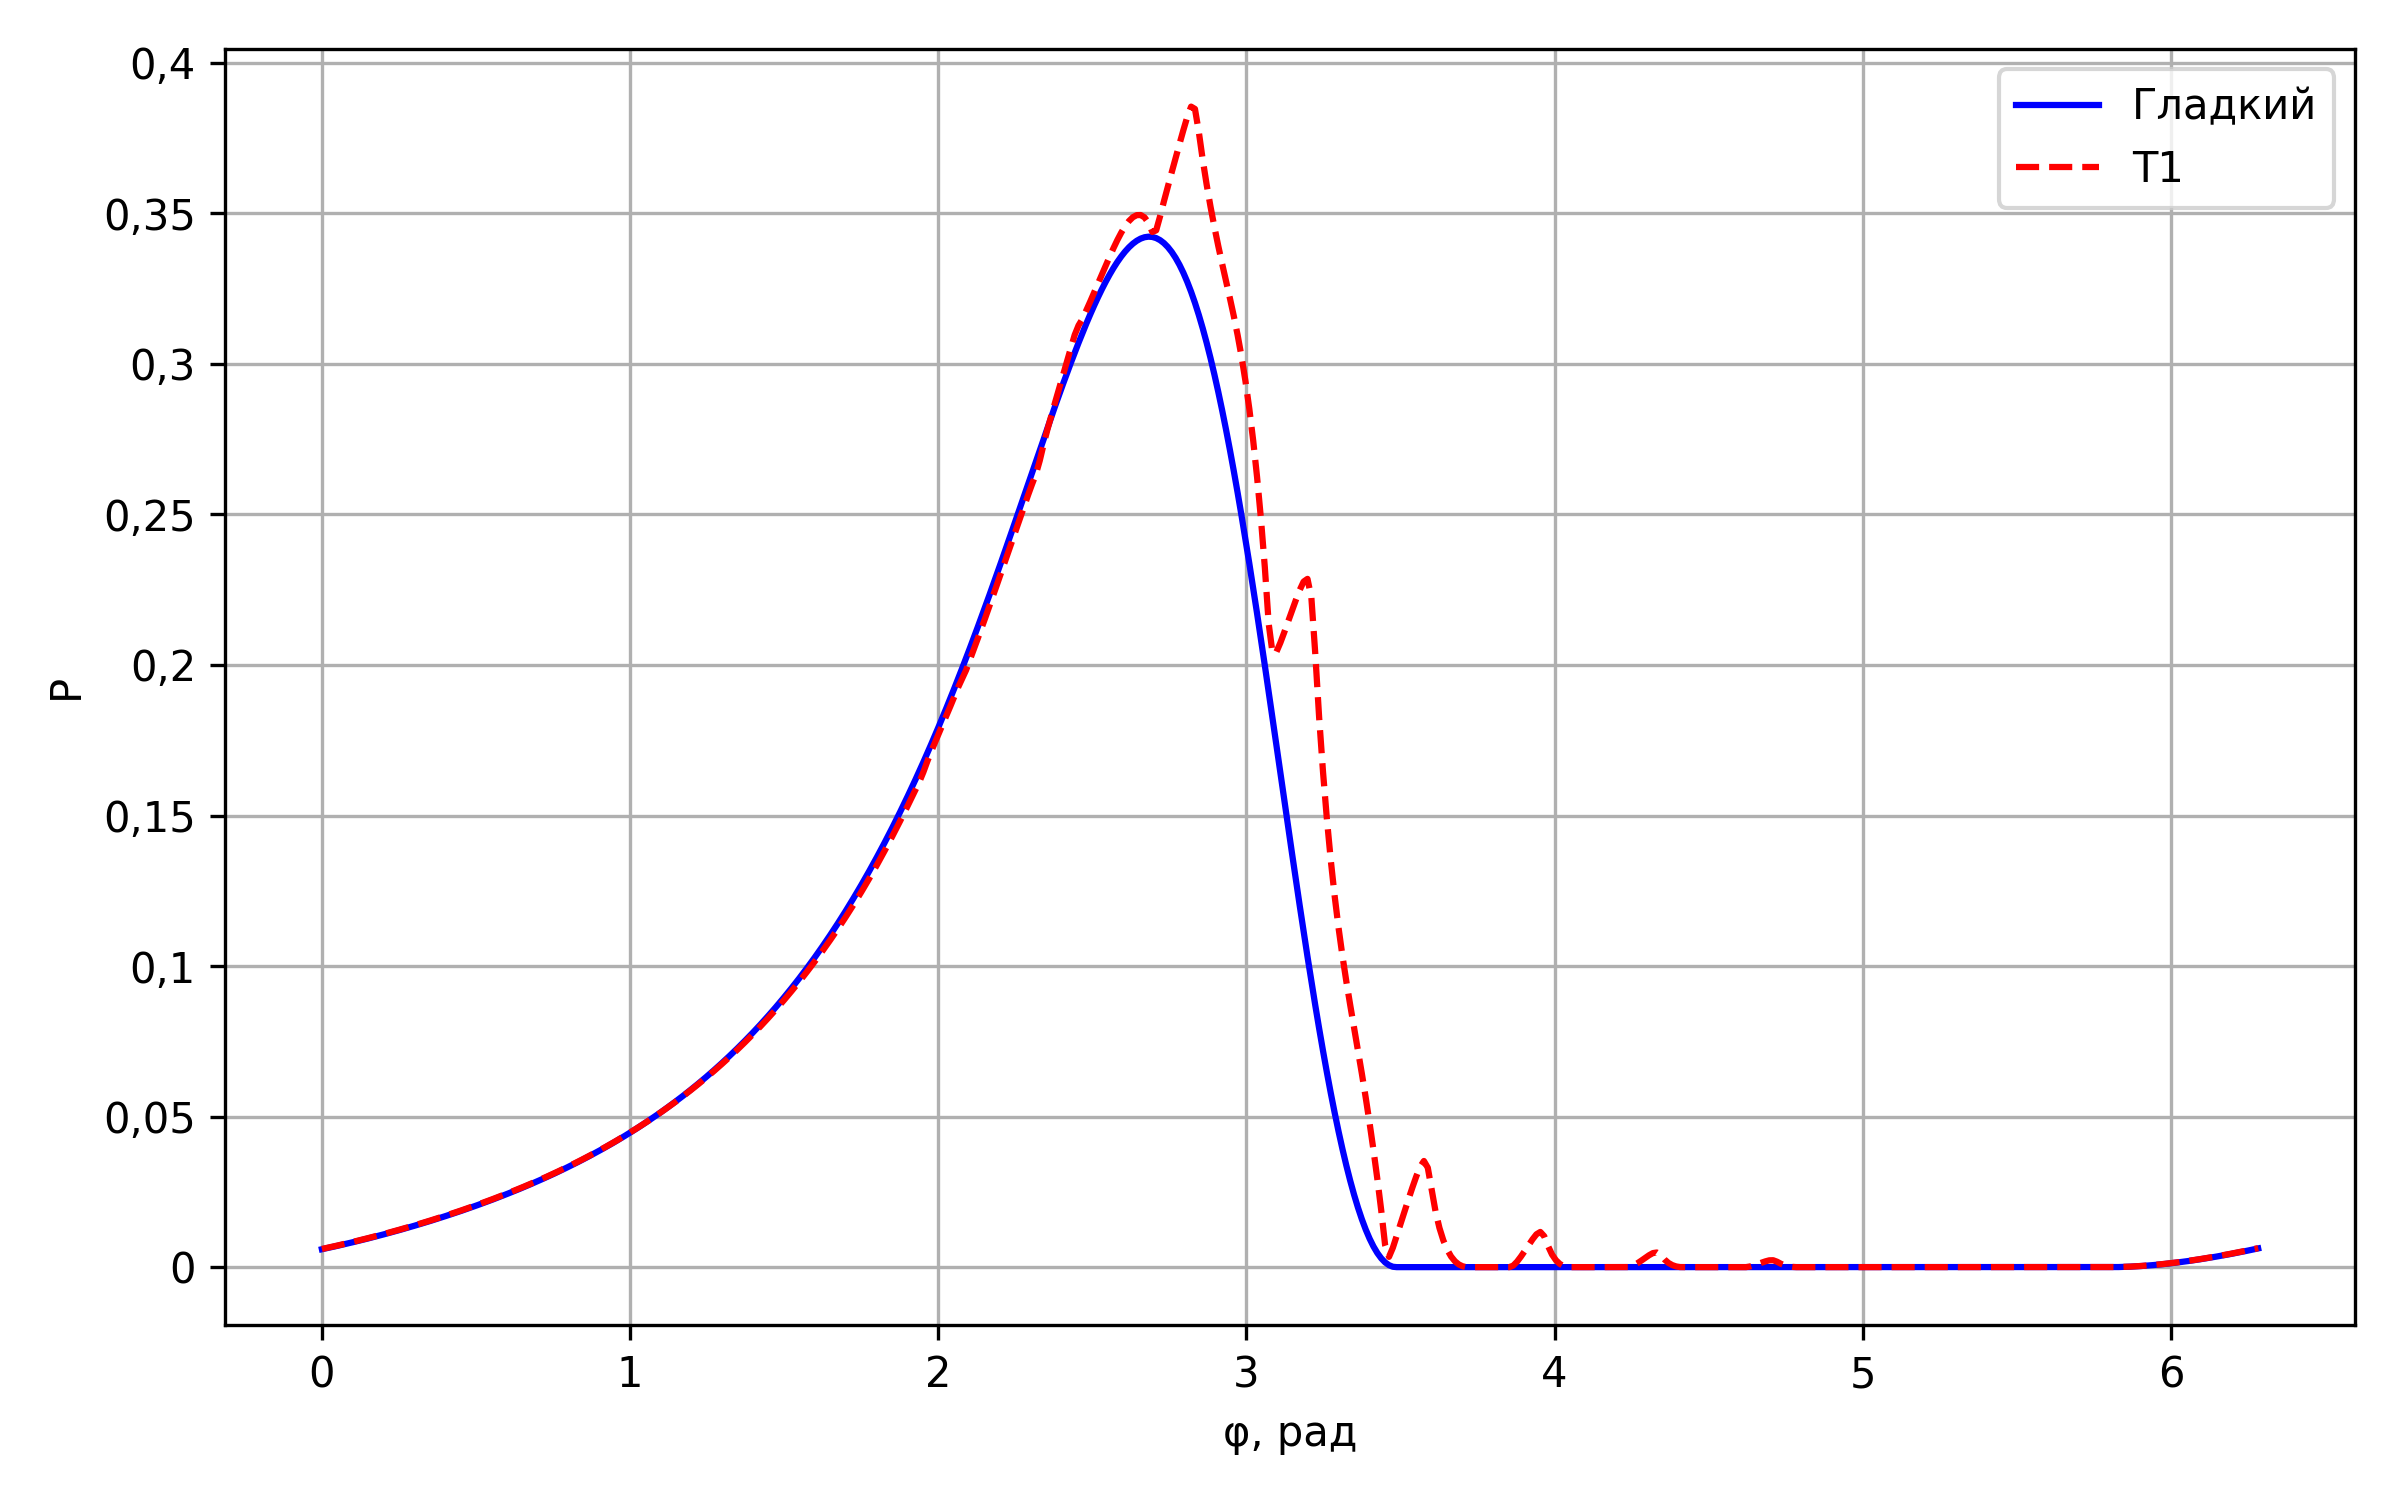
\includegraphics[width=0.75\textwidth]{figures/ch05/fig_5_14.png}
\caption{Распределение безразмерного давления $P(\theta)$ при $Z = 0$
  для гладкого подшипника и конфигурации~T1 ($\varepsilon = 0{,}6$).
  Вторичные пики на кривой T1 соответствуют лункам,
  расположенным в зоне $90^{\circ}$--$270^{\circ}$.}
\label{fig:comparison_curves}
\end{figure}

\begin{figure}[!ht]
\centering
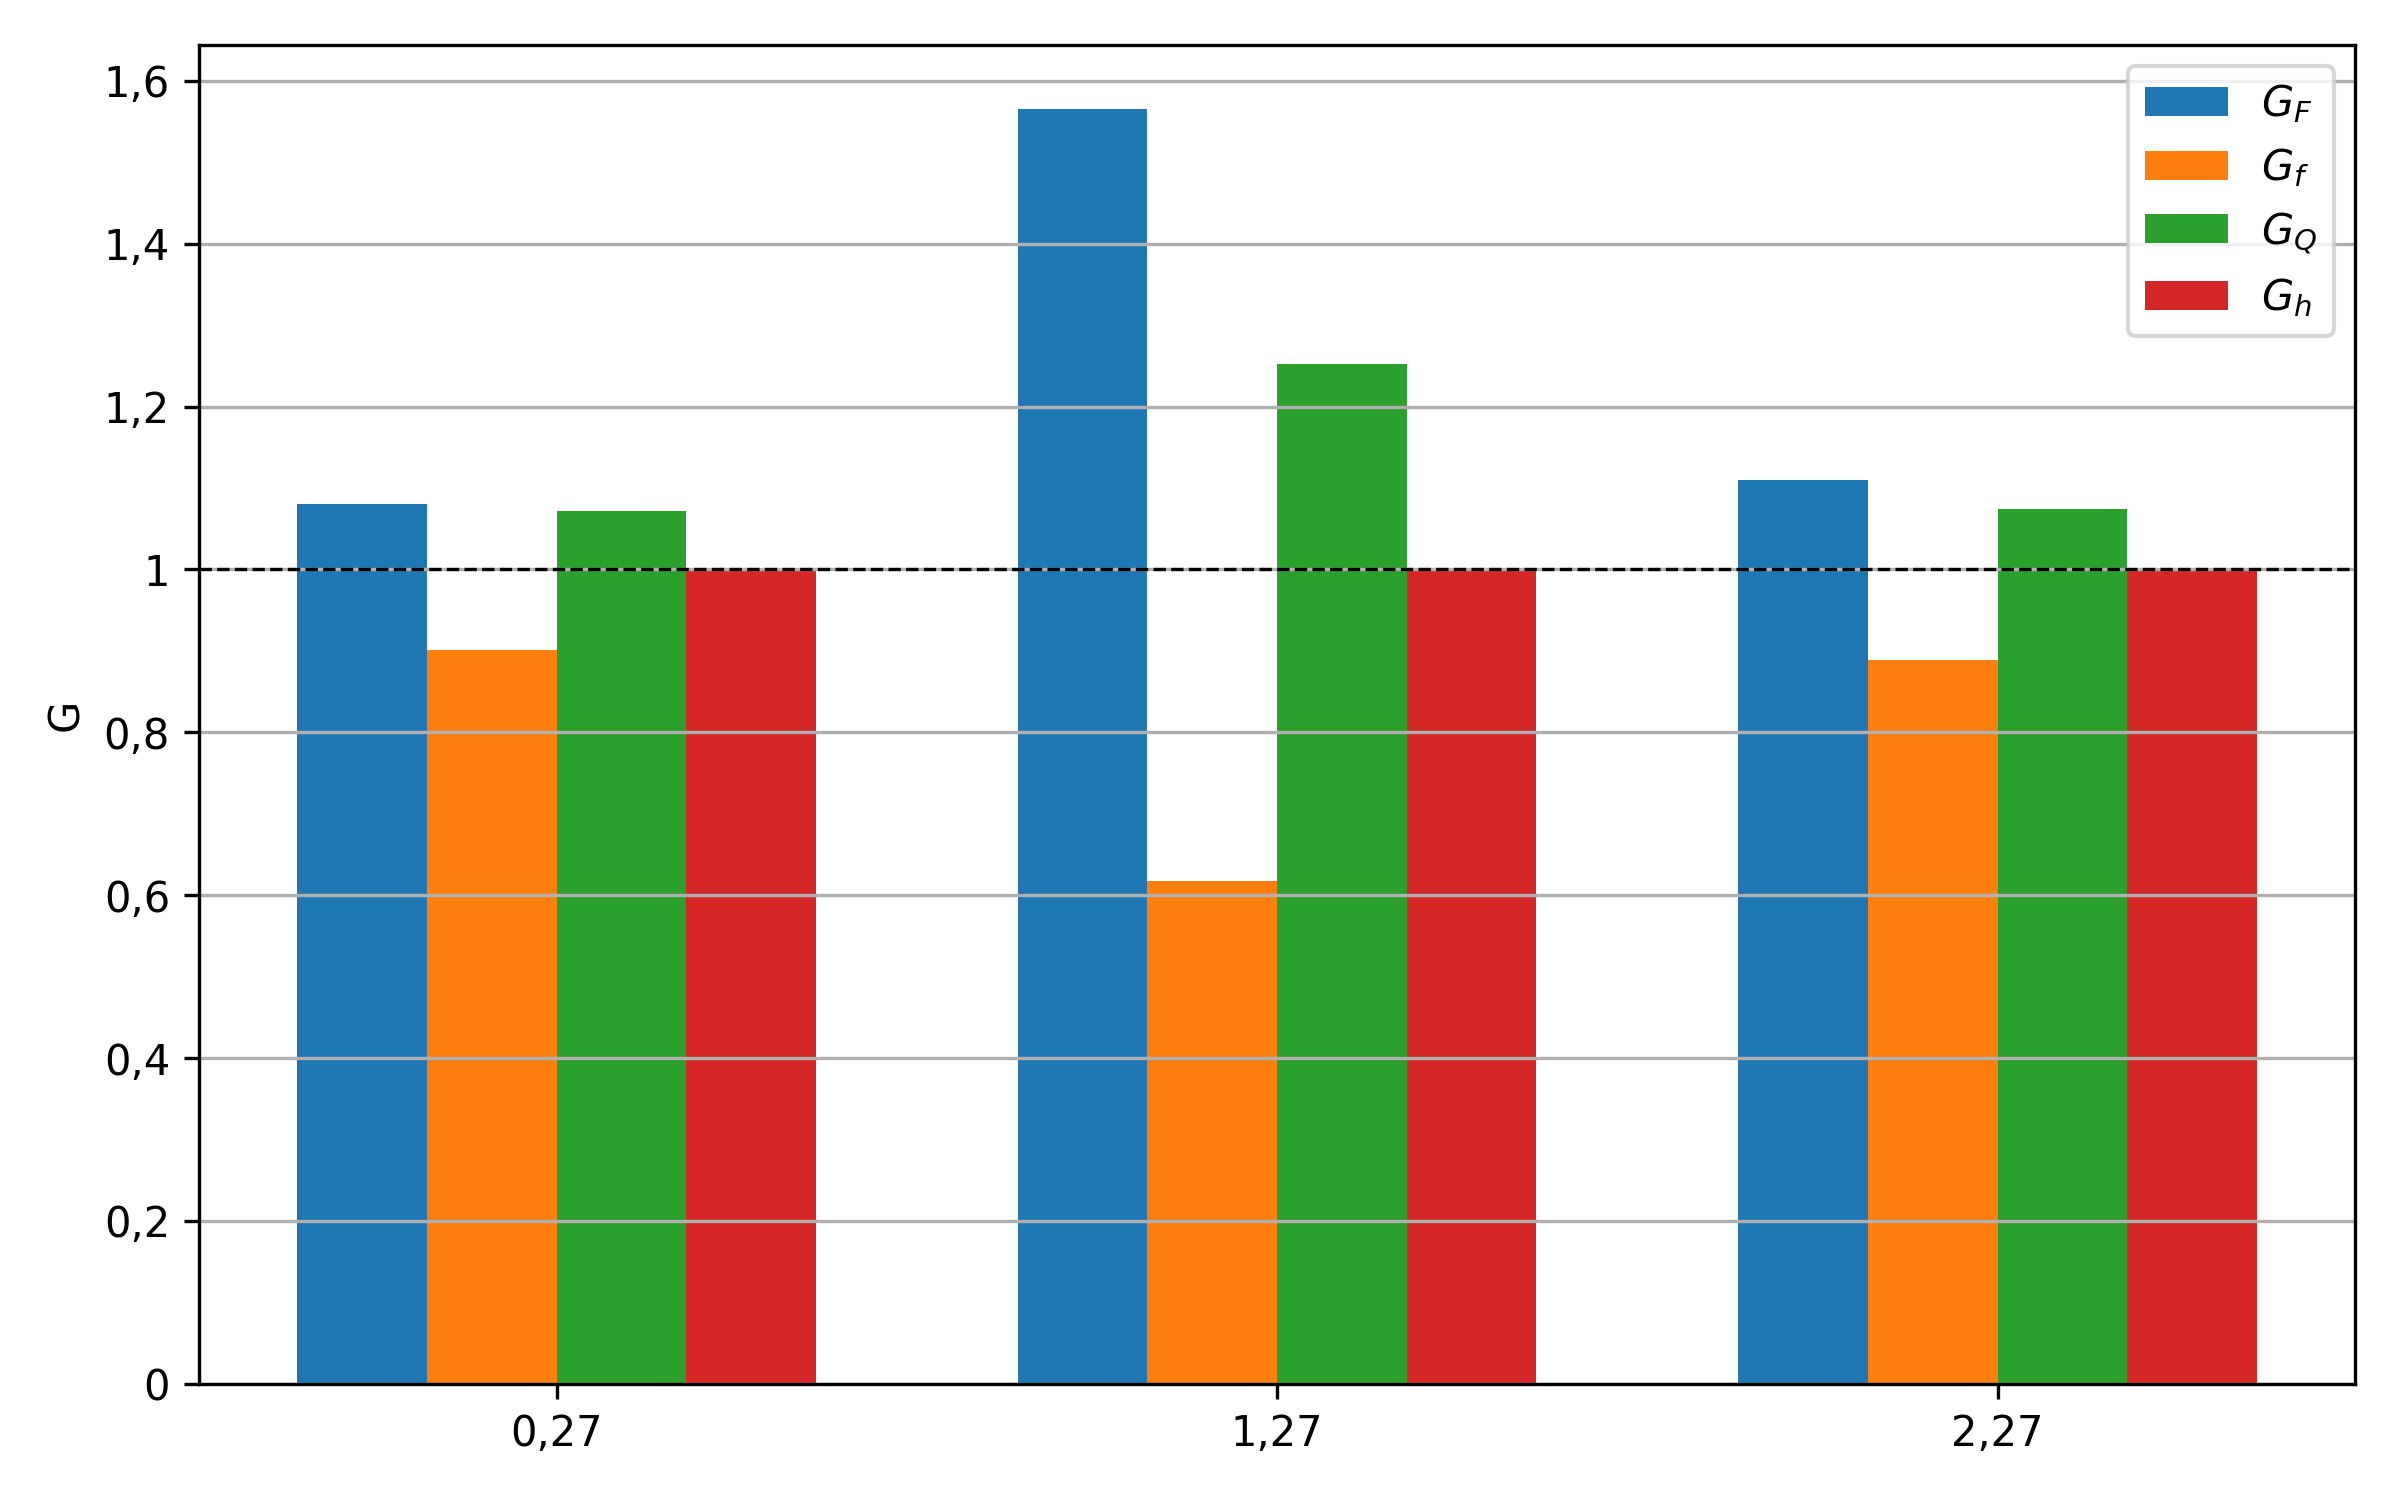
\includegraphics[width=0.75\textwidth]{figures/ch05/fig_5_15.png}
\caption{Нормированные показатели эффективности текстурирования $G_F$, $G_f$,
  $G_Q$, $G_h$ для конфигураций T1, T2, T3 при $\varepsilon = 0{,}6$.
  Пунктирная горизонталь $G = 1$ соответствует уровню гладкого подшипника.}
\label{fig:gains_nom}
\end{figure}

\FloatBarrier

\textit{Нагрузочные характеристики.}
Зависимости несущей способности~$F(\varepsilon)$
и коэффициента трения~$\mu_f(\varepsilon)$ для гладкого
и текстурированного подшипников позволяют оценить эффективность
текстурирования во всём диапазоне рабочих эксцентриситетов.
При малых эксцентриситетах ($\varepsilon \ll 1$), когда зазор
близок к равномерному, влияние микроструктур наиболее выражено:
каждая лунка вносит вклад, сопоставимый с макроскопическим
клиновым эффектом. С ростом~$\varepsilon$ собственный
гидродинамический эффект клинового зазора подшипника усиливается
и начинает доминировать, а относительный вклад текстуры
снижается. Графики нагрузочных характеристик для всех вариантов
представлены на рисунках~\ref{fig:F_vs_epsilon},
\ref{fig:mu_vs_epsilon}, \ref{fig:Q_vs_epsilon}.


\FloatBarrier
\section*{Выводы по главе~5}
\phantomsection\addcontentsline{toc}{section}{Выводы по главе~5}

Проведён статический анализ радиального подшипника скольжения
центробежного насоса в изотермическом приближении с учётом
кавитации по условию Рейнольдса ($P \geq 0$).

Для гладкого подшипника получены поля давления и установлены
границы кавитационной зоны при различных значениях
эксцентриситета. Зависимости несущей
способности~$F(\varepsilon)$, коэффициента
трения~$\mu_f(\varepsilon)$ и осевых
утечек~$Q_{\mathrm{out}}(\varepsilon)$ демонстрируют
характерное поведение гидродинамического подшипника~\cite{rakhonde2018,manshoor2013,madhusudhanarao2020}: рост
несущей способности и убывание коэффициента трения
с увеличением~$\varepsilon$, а также возрастание осевых утечек,
обусловленное ростом перепада давления в осевом направлении~\cite{christiansen2017,zhang2015,fernandes2012}.

Текстурирование поверхности вкладыша эллипсоидальными лунками
в шахматной раскладке модифицирует поле давления: в зоне
расположения элементов возникают локальные возмущения давления,
формируемые микроклиновым эффектом каждой лунки. Конфигурация
кавитационной зоны при текстурировании отличается от эталонного
случая гладкого подшипника~\cite{shenoy2010,elsaid2017}.

Сравнение интегральных характеристик по нормированным
показателям~$G_F$, $G_f$, $G_Q$, $G_h$~\eqref{eq:gain_factors}
при $\varepsilon = 0{,}6$ показывает: конфигурация~T2
($H_p = 0{,}40$, зона $90^{\circ}$--$270^{\circ}$) обеспечивает
наибольший прирост несущей способности ($G_F = 1{,}566$)
и снижение трения ($G_f = 0{,}617$); конфигурации~T1
и~T3 ($H_p = 0{,}20$) показывают умеренный эффект
($G_F \approx 1{,}08$--$1{,}11$, $G_f \approx 0{,}89$--$0{,}90$).
Показатель $G_h = 1{,}00$ для всех конфигураций подтверждает,
что минимальный зазор определяется эксцентриситетом, а не
геометрией лунок.

Эффективность текстурирования существенно зависит от глубины
элементов~$H_p$; влияние зоны нанесения при умеренной глубине
($H_p = 0{,}20$) выражено слабо. Глубина элементов
и коэффициент покрытия~$\varphi$ должны быть согласованы
с рабочим диапазоном эксцентриситетов.

При больших эксцентриситетах ($\varepsilon \to 1$) влияние
микроструктур ослабевает, поскольку макроскопический клиновой
эффект доминирует; в этом режиме текстурирование оказывается
нейтральным или малоэффективным.

Анализ радиального подшипника для иного класса объектов~--
опоры шарошечного долота~-- выполнен в главе~6. Упорный
подшипник рассмотрен в главе~7. Влияние микроструктур
на динамические характеристики подшипника (коэффициенты
жёсткости и демпфирования, устойчивость ротора) составляет
предмет главы~8.



\section{Пример анализа радиального подшипника шарошечного долота}

Второй пример посвящён расчёту радиального подшипника скольжения опоры шарошечного долота. В~отличие от~предыдущего примера, данный подшипник работает при~существенно меньшей скорости скольжения и~более высокой удельной нагрузке, что~обуславливает иной характер результатов и~выводов. Пример иллюстрирует, как~текстурирование поверхности может существенно повысить несущую способность подшипника в~тяжёлых условиях эксплуатации.

% =============================================================
% 6 Анализ радиального подшипника шарошечного долота
% =============================================================
\chapter{Анализ рельефного радиального подшипника шарошечного долота}

\section{Объект исследования и исходные данные}

Объектом исследования в настоящей главе является радиальный
подшипник скольжения опоры шарошки трёхшарошечного долота~\cite{bashmur2024a,bashmur2024b}.
Цапфа (лапа долота) неподвижна относительно корпуса; шарошка
вращается вокруг цапфы. Подшипниковый узел воспринимает
радиальные нагрузки от долота и обеспечивает смазку при тяжёлых
условиях эксплуатации: высокие нагрузки, низкая скорость
скольжения, ограниченная подача смазки.

В отличие от подшипника насоса (глава~5), опора шарошечного долота
работает при скорости скольжения~$U_{\mathrm{eq}}$, примерно
в~90 раз меньшей, и нагрузке $F_{\mathrm{ext}} = 6\,000$~Н на цапфу. Вследствие малой
скорости гидродинамическое давление невелико, и подшипник
функционирует в смешанном или граничном режиме смазки. Применение
детерминированных микроструктур рабочей поверхности направлено
на повышение гидродинамической составляющей несущей способности
и улучшение условий смазки~\cite{bashmur2022,bashmur2023a,bashmur2023b,guo2005}.

Кинематика узла определяется вращением шарошки. Угловая скорость
вращения долота (корпуса):
\begin{equation}
  \omega = \frac{2\pi n}{60},
  \label{eq:bit_omega}
\end{equation}
где $n$~-- частота вращения долота, об/мин. Относительная угловая
скорость шарошки относительно цапфы:
\begin{equation}
  \omega_{\mathrm{rel}} = \omega
    \left(\frac{R_b}{R_k} - 1\right),
  \label{eq:bit_omega_rel}
\end{equation}
где $R_b$~-- радиус долота, $R_k$~-- радиус шарошки.
Эквивалентная скорость скольжения на поверхности цапфы:
\begin{equation}
  U_{\mathrm{eq}} = |\omega_{\mathrm{rel}}|\, R,
  \label{eq:bit_Ueq}
\end{equation}
где $R$~-- радиус цапфы. Подстановка числовых значений даёт
$U_{\mathrm{eq}} \approx 0{,}124$~м/с.

Нагрузка на цапфу определяется из осевой нагрузки на долото~$F_a$.
Нагрузка на одну шарошку при равномерном распределении:
\begin{equation}
  F_{\mathrm{cone}} = \frac{F_a}{3}.
  \label{eq:bit_Fcone}
\end{equation}
В расчётах принято $F_a = 150$~кН, что соответствует
$F_{\mathrm{cone}} = 50$~кН.
Радиальная нагрузка на цапфу:
\begin{equation}
  F_{\mathrm{ext}} = k_L \cdot F_{\mathrm{cone}},
  \label{eq:bit_Fext}
\end{equation}
где $k_L = 0{,}12$~-- коэффициент передачи нагрузки на цапфу
(инженерное оценочное допущение; далее принято $k_L = 0{,}12$).

Основные параметры подшипника сведены в таблицу~\ref{tab:bit_params}.

\begin{table}[!ht]
\centering
\caption{Параметры радиального подшипника скольжения опоры шарошки}
\label{tab:bit_params}
\begin{tabularx}{\textwidth}{|X|c|c|c|}
\hline
\multicolumn{1}{|c|}{\textbf{Параметр}} & \textbf{Обозначение} & \textbf{Значение} & \textbf{Единица} \\
\hline
Радиус цапфы              & $R$              & 30{,}0  & мм \\
\hline
Длина подшипника          & $L$              & 40{,}0  & мм \\
\hline
Радиальный зазор          & $c$              & 60      & мкм \\
\hline
Относительный зазор       & $\psi = c/R$     & $2{,}00 \times 10^{-3}$ & -- \\
\hline
Отношение $L/D$           & $L/D$            & 0{,}667 & -- \\
\hline
Радиус долота             & $R_b$            & 107{,}5 & мм \\
\hline
Радиус шарошки            & $R_k$            & 72{,}0  & мм \\
\hline
Частота вращения          & $n$              & 80      & об/мин \\
\hline
Угловая скорость          & $\omega$         & 8{,}38  & рад/с \\
\hline
Эквивалентная скорость    & $U_{\mathrm{eq}}$ & 0{,}124 & м/с \\
\hline
Динамическая вязкость     & $\mu_0$          & $5{,}5 \times 10^{-2}$ & Па$\cdot$с \\
\hline
Температура               & $T_0$            & 80      & $^{\circ}$C \\
\hline
Суммарная шероховатость   & $\sigma_{\mathrm{eq}}$ & 0{,}89 & мкм \\
\hline
Коэффициент передачи      & $k_L$            & 0{,}12  & -- \\
\hline
Нагрузка на цапфу         & $F_{\mathrm{ext}}$ & 6\,000 & Н \\
\hline
Давление кавитации        & $p_{\mathrm{cav}}$ & 0     & Па \\
\hline
\end{tabularx}
\end{table}

\FloatBarrier

Схема опоры шарошки представлена на рисунке~\ref{fig:bit_scheme}.

\begin{figure}[!ht]
\centering
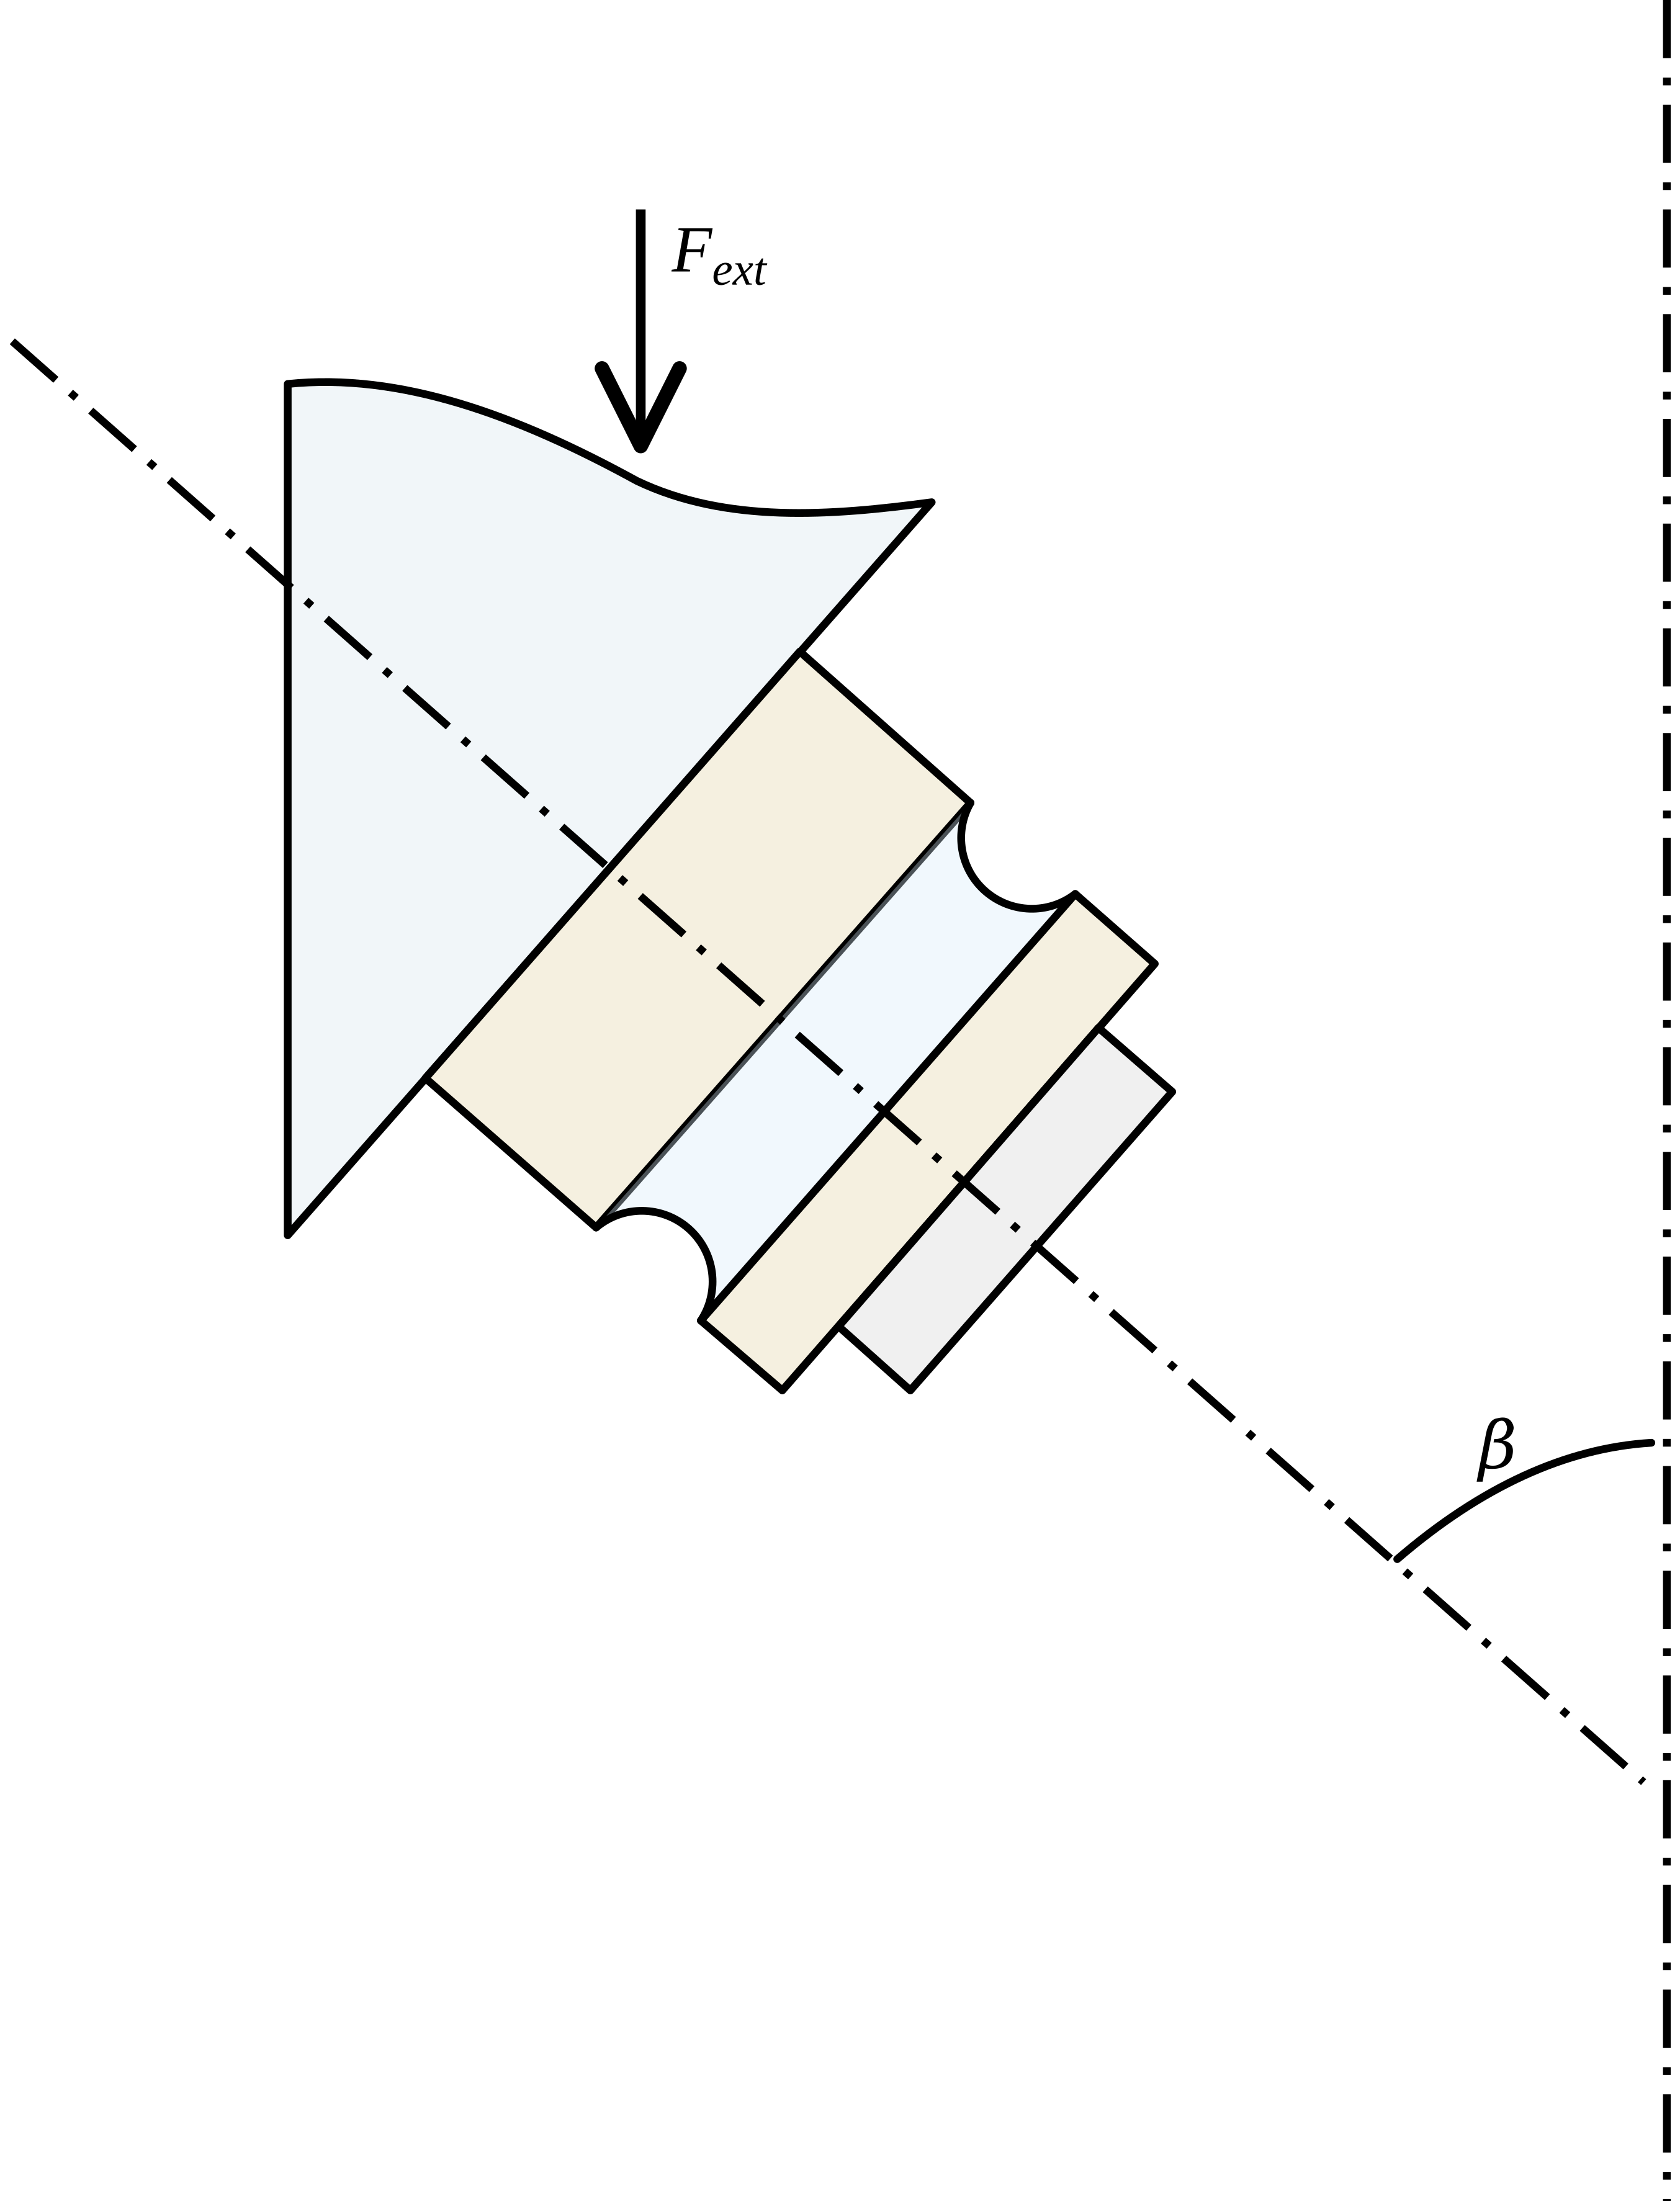
\includegraphics[width=\textwidth,height=0.9\textheight,keepaspectratio]{figures/ch06/fig_6_1.png}
\caption{Схема опоры шарошки трёхшарошечного долота}
\label{fig:bit_scheme}
\end{figure}

\FloatBarrier


\section{Постановка задачи}\label{sec:problem_statement_ch6}

Расчётная область представляет собой развёрнутую поверхность
смазочного зазора $(\theta, z) \in [0,\,2\pi] \times [-L/2,\,L/2]$,
где $\theta$~-- окружная координата, $z$~-- осевая координата.
В тексте главы окружная координата обозначается~$\theta$;
на рисунках ось подписана~$\varphi$; везде $\theta \equiv \varphi$.
При переходе к безразмерным переменным (подраздел~2.1.6)
осевая координата нормируется на полудлину: $Z = 2z/L$,
так что $Z \in [-1,\,1]$.

Для гладкого цилиндрического подшипника безразмерная толщина
зазора определяется законом~\eqref{eq:journal_h_ch5}:
\begin{equation}
  H(\theta) = 1 + \varepsilon\cos\theta,
  \label{eq:bit_h}
\end{equation}
где $\varepsilon = e/c$~-- относительный эксцентриситет
($0 \leq \varepsilon < 1$). Для подшипника с детерминированными
микроструктурами толщина зазора записывается в виде
суперпозиции~\eqref{eq:journal_h_tex_ch5}:
\begin{equation}
  H = H_0(\theta) + \Delta H_t(\theta, Z).
  \label{eq:bit_h_tex}
\end{equation}
где $H_0(\theta) = 1 + \varepsilon\cos\theta$~-- базовый зазор гладкого подшипника~\eqref{eq:bit_h}, $\Delta H_t$~-- добавка микрорельефа (подраздел~2.2).

Распределение давления описывается безразмерным уравнением
Рейнольдса~\eqref{eq:reynolds_nondim} с параметром
анизотропии~$\Lambda$~\eqref{eq:nondim_Lambda}.

Граничные условия: по окружной координате~$\theta$ поле давления
периодично ($P(\theta = 0) = P(\theta = 2\pi)$); на торцах
подшипника давление равно атмосферному ($P = 0$ при $Z = \pm 1$).
Кавитация учитывается по условию Рейнольдса: $P \geq 0$.

В отличие от главы~5, где эксцентриситет задавался как входной
параметр и вычислялась несущая сила~$F(\varepsilon)$, в настоящей
главе рассматривается обратная задача: задаётся внешняя нагрузка
$F_{\mathrm{ext}}$, а равновесный эксцентриситет~$\varepsilon^*$
определяется из условия равновесия:
\begin{equation}
  F(\varepsilon^*) = F_{\mathrm{ext}}.
  \label{eq:bit_equilibrium}
\end{equation}
Решение уравнения~\eqref{eq:bit_equilibrium} выполняется методом
бисекции по~$\varepsilon \in [0{,}05;\; 0{,}97]$ с допуском~$1\,\%$.

Для оценки режима смазки вводится минимальная толщина плёнки:
\begin{equation}
  h_{\min} = c\,(1 - \varepsilon),
  \label{eq:bit_hmin}
\end{equation}
а также параметр плёнки:
\begin{equation}
  \lambda = \frac{h_{\min}}{\sigma_{\mathrm{eq}}},
  \label{eq:bit_lambda}
\end{equation}
где $\sigma_{\mathrm{eq}}$~-- суммарная шероховатость поверхностей.
Классификация режимов смазки по параметру~$\lambda$:
$\lambda < 1$~-- граничный режим;
$1 \leq \lambda \leq 3$~-- смешанный режим;
$\lambda > 3$~-- гидродинамический режим.

Для сравнительной оценки условий работы узла вводится
$PV$-параметр:
\begin{equation}
  p_0 = \frac{F}{2\,R\,L}, \qquad
  PV = p_0 \cdot U_{\mathrm{eq}},
  \label{eq:bit_PV}
\end{equation}
и индекс износа:
\begin{equation}
  I_w = \frac{PV}{h_{\min}}.
  \label{eq:bit_Iw}
\end{equation}
Величина~$I_w$ является суррогатным сравнительным
индексом, характеризующим интенсивность изнашивания; строгое
соответствие закону Арчарда не предполагается.

Допущения, принятые в настоящей главе, включают: изотермическое
приближение ($T = T_0$, $\mu = \mathrm{const}$), постоянство
плотности ($\rho = \mathrm{const}$) и кавитация по условию
Рейнольдса ($P \geq 0$).


\section{Результаты для гладкого подшипника}

При расчётном пределе эксцентриситета $\varepsilon = 0{,}97$
гладкий подшипник развивает несущую силу
$F(\varepsilon = 0{,}97) = 1907$~Н. Это составляет около~$3{,}8\,\%$
от нагрузки на шарошку $F_{\mathrm{cone}} = F_a / 3 = 50\,000$~Н
и менее трети рабочей нагрузки $F_{\mathrm{ext}} = 6\,000$~Н.

Низкая несущая способность обусловлена малой скоростью скольжения
$U_{\mathrm{eq}} \approx 0{,}124$~м/с, примерно в~90 раз меньшей,
чем у подшипника насоса главы~5. Гидродинамическое давление
пропорционально скорости ($p \sim \mu_0\, U_{\mathrm{eq}}\, R / c^2$), поэтому даже
при предельном эксцентриситете несущая сила не достигает
$F_{\mathrm{ext}}$.

При рабочей нагрузке $F_{\mathrm{ext}} = 6\,000$~Н гладкий
подшипник не имеет равновесной рабочей точки в чисто
гидродинамической постановке. Режим смазки~-- смешанный или
граничный. Применение детерминированных микроструктур
рассматривается как средство повышения гидродинамической
составляющей несущей способности.


\section{Выбор и параметры микроструктуры}

В качестве элементов микрорельефа выбраны эллипсоидальные лунки
с профилем~\eqref{eq:profile_ellipsoidal}, расположенные
по шахматной схеме~\eqref{eq:layout_staggered}. Выбор типа
элемента и раскладки аналогичен главе~5 (подраздел~2.2).

Зона нанесения микроструктур определяется расположением области
максимального давления. В радиальном подшипнике максимум давления
формируется вблизи $\theta \approx \pi$ (зона минимального зазора).
Конфигурации~T1 и~T2 нанесены в секторе
$90^{\circ}$--$270^{\circ}$, включающем эту зону. Конфигурация~T3
нанесена в секторе $0^{\circ}$--$180^{\circ}$ (зона сходящегося
клина).

Параметры микроструктур (безразмерные полуоси~$A^*$, $B^*$)
пересчитаны под геометрию опоры шарошки ($R = 30$~мм,
$L = 40$~мм); числовые значения отличаются от конфигураций
главы~5 ($R = 35$~мм, $L = 56$~мм). Поэтому сравнение текстур
выполняется только внутри настоящей главы; прямое количественное
сопоставление с главой~5 не проводится.

Параметры рассматриваемых конфигураций приведены в
таблице~\ref{tab:bit_texture_configs}.

\begin{table}[!ht]
\centering
\caption{Параметры конфигураций текстуры для подшипника шарошечного долота}
\label{tab:bit_texture_configs}
\begin{tabularx}{\textwidth}{|X|c|c|c|c|}
\hline
\multicolumn{1}{|c|}{\textbf{Конфигурация}} & $\boldsymbol{H_p}$ & $\boldsymbol{A^*}$ & $\boldsymbol{B^*}$ & \textbf{Зона нанесения} \\
\hline
T1 & 0{,}20 & 0{,}0600 & 0{,}0367 & $90^{\circ}$--$270^{\circ}$ \\
\hline
T2 & 0{,}40 & 0{,}0600 & 0{,}0367 & $90^{\circ}$--$270^{\circ}$ \\
\hline
T3 & 0{,}20 & 0{,}0600 & 0{,}0367 & $0^{\circ}$--$180^{\circ}$ \\
\hline
\end{tabularx}
\end{table}


\section{Сравнение гладкого и текстурированного подшипников}

\textit{Рабочие точки при заданной нагрузке на цапфу.}
Все три конфигурации текстуры (T1--T3) обеспечивают равновесную
рабочую точку при $F_{\mathrm{ext}} = 6\,000$~Н; гладкий
подшипник рабочей точки не имеет. Результаты расчёта рабочих точек
сведены в таблицу~\ref{tab:bit_results}.

\begin{table}[!ht]
\centering
\caption{Характеристики подшипника в рабочей точке
  при $F_{\mathrm{ext}} = 6\,000$~Н}
\label{tab:bit_results}
\resizebox{\textwidth}{!}{%
\begin{tabular}{|l|c|c|c|c|c|c|c|c|}
\hline
\multicolumn{1}{|c|}{\textbf{Вар.}}
  & $\boldsymbol{\varepsilon}$
  & $\boldsymbol{F}$, Н
  & $\boldsymbol{\varphi}$, $^{\circ}$
  & $\boldsymbol{\mu_f}$
  & $\boldsymbol{h_{\min}}$, мкм
  & $\boldsymbol{\lambda}$
  & $\boldsymbol{PV}$, Па$\cdot$м/с
  & $\boldsymbol{I_w}$ \\
\hline
T1 & 0{,}966 & 6004 & 175{,}4 & 0{,}00123 & 2{,}04 & 2{,}28
   & 309\,981 & $1{,}5 \cdot 10^{11}$ \\
\hline
T2 & 0{,}956 & 6044 & 175{,}9 & 0{,}00107 & 2{,}66 & 2{,}98
   & 312\,090 & $1{,}2 \cdot 10^{11}$ \\
\hline
T3 & 0{,}969 & 5956 & 173{,}8 & 0{,}00136 & 1{,}85 & 2{,}07
   & 307\,503 & $1{,}7 \cdot 10^{11}$ \\
\hline
\end{tabular}%
}
\end{table}

\FloatBarrier

Все три конфигурации работают в смешанном режиме смазки
($1 \leq \lambda \leq 3$).

Приведённый коэффициент трения~$\mu_f$ соответствует
гидродинамической составляющей модели. В смешанном режиме
($\lambda < 3$) реальное трение в узле выше вследствие
дополнительного вклада контактного взаимодействия шероховатостей
поверхностей.

Конфигурация~T2 демонстрирует наилучшие характеристики:
наименьший эксцентриситет $\varepsilon = 0{,}956$, наибольший
минимальный зазор $h_{\min} = 2{,}66$~мкм, параметр плёнки
$\lambda = 2{,}98$~-- значение, наиболее близкое к границе
гидродинамического режима. Конфигурация~T3, в которой текстура
расположена вне зоны максимального давления, показывает наихудшие
значения~$h_{\min}$ и~$\lambda$.


\textit{Грузоподъёмность при расчётном пределе эксцентриситета.}
При расчётном пределе $\varepsilon = 0{,}97$ несущая сила
составляет: гладкий подшипник~-- $1\,907$~Н; T1~-- $7\,237$~Н;
T2~-- $7\,549$~Н; T3~-- $6\,212$~Н. Максимальная грузоподъёмность
конфигурации~T2 в~$3{,}96$ раза превышает значение гладкого
подшипника. Горизонталь $F_{\mathrm{ext}} = 6\,000$~Н пересекает
кривые~T1, T2, T3, но не кривую гладкого подшипника: рабочая точка
при заданной нагрузке существует только при наличии текстуры.

Зависимости несущей силы~$F(\varepsilon)$ для всех вариантов
представлены на рисунке~\ref{fig:bit_operating_points}.

\begin{figure}[!ht]
\centering
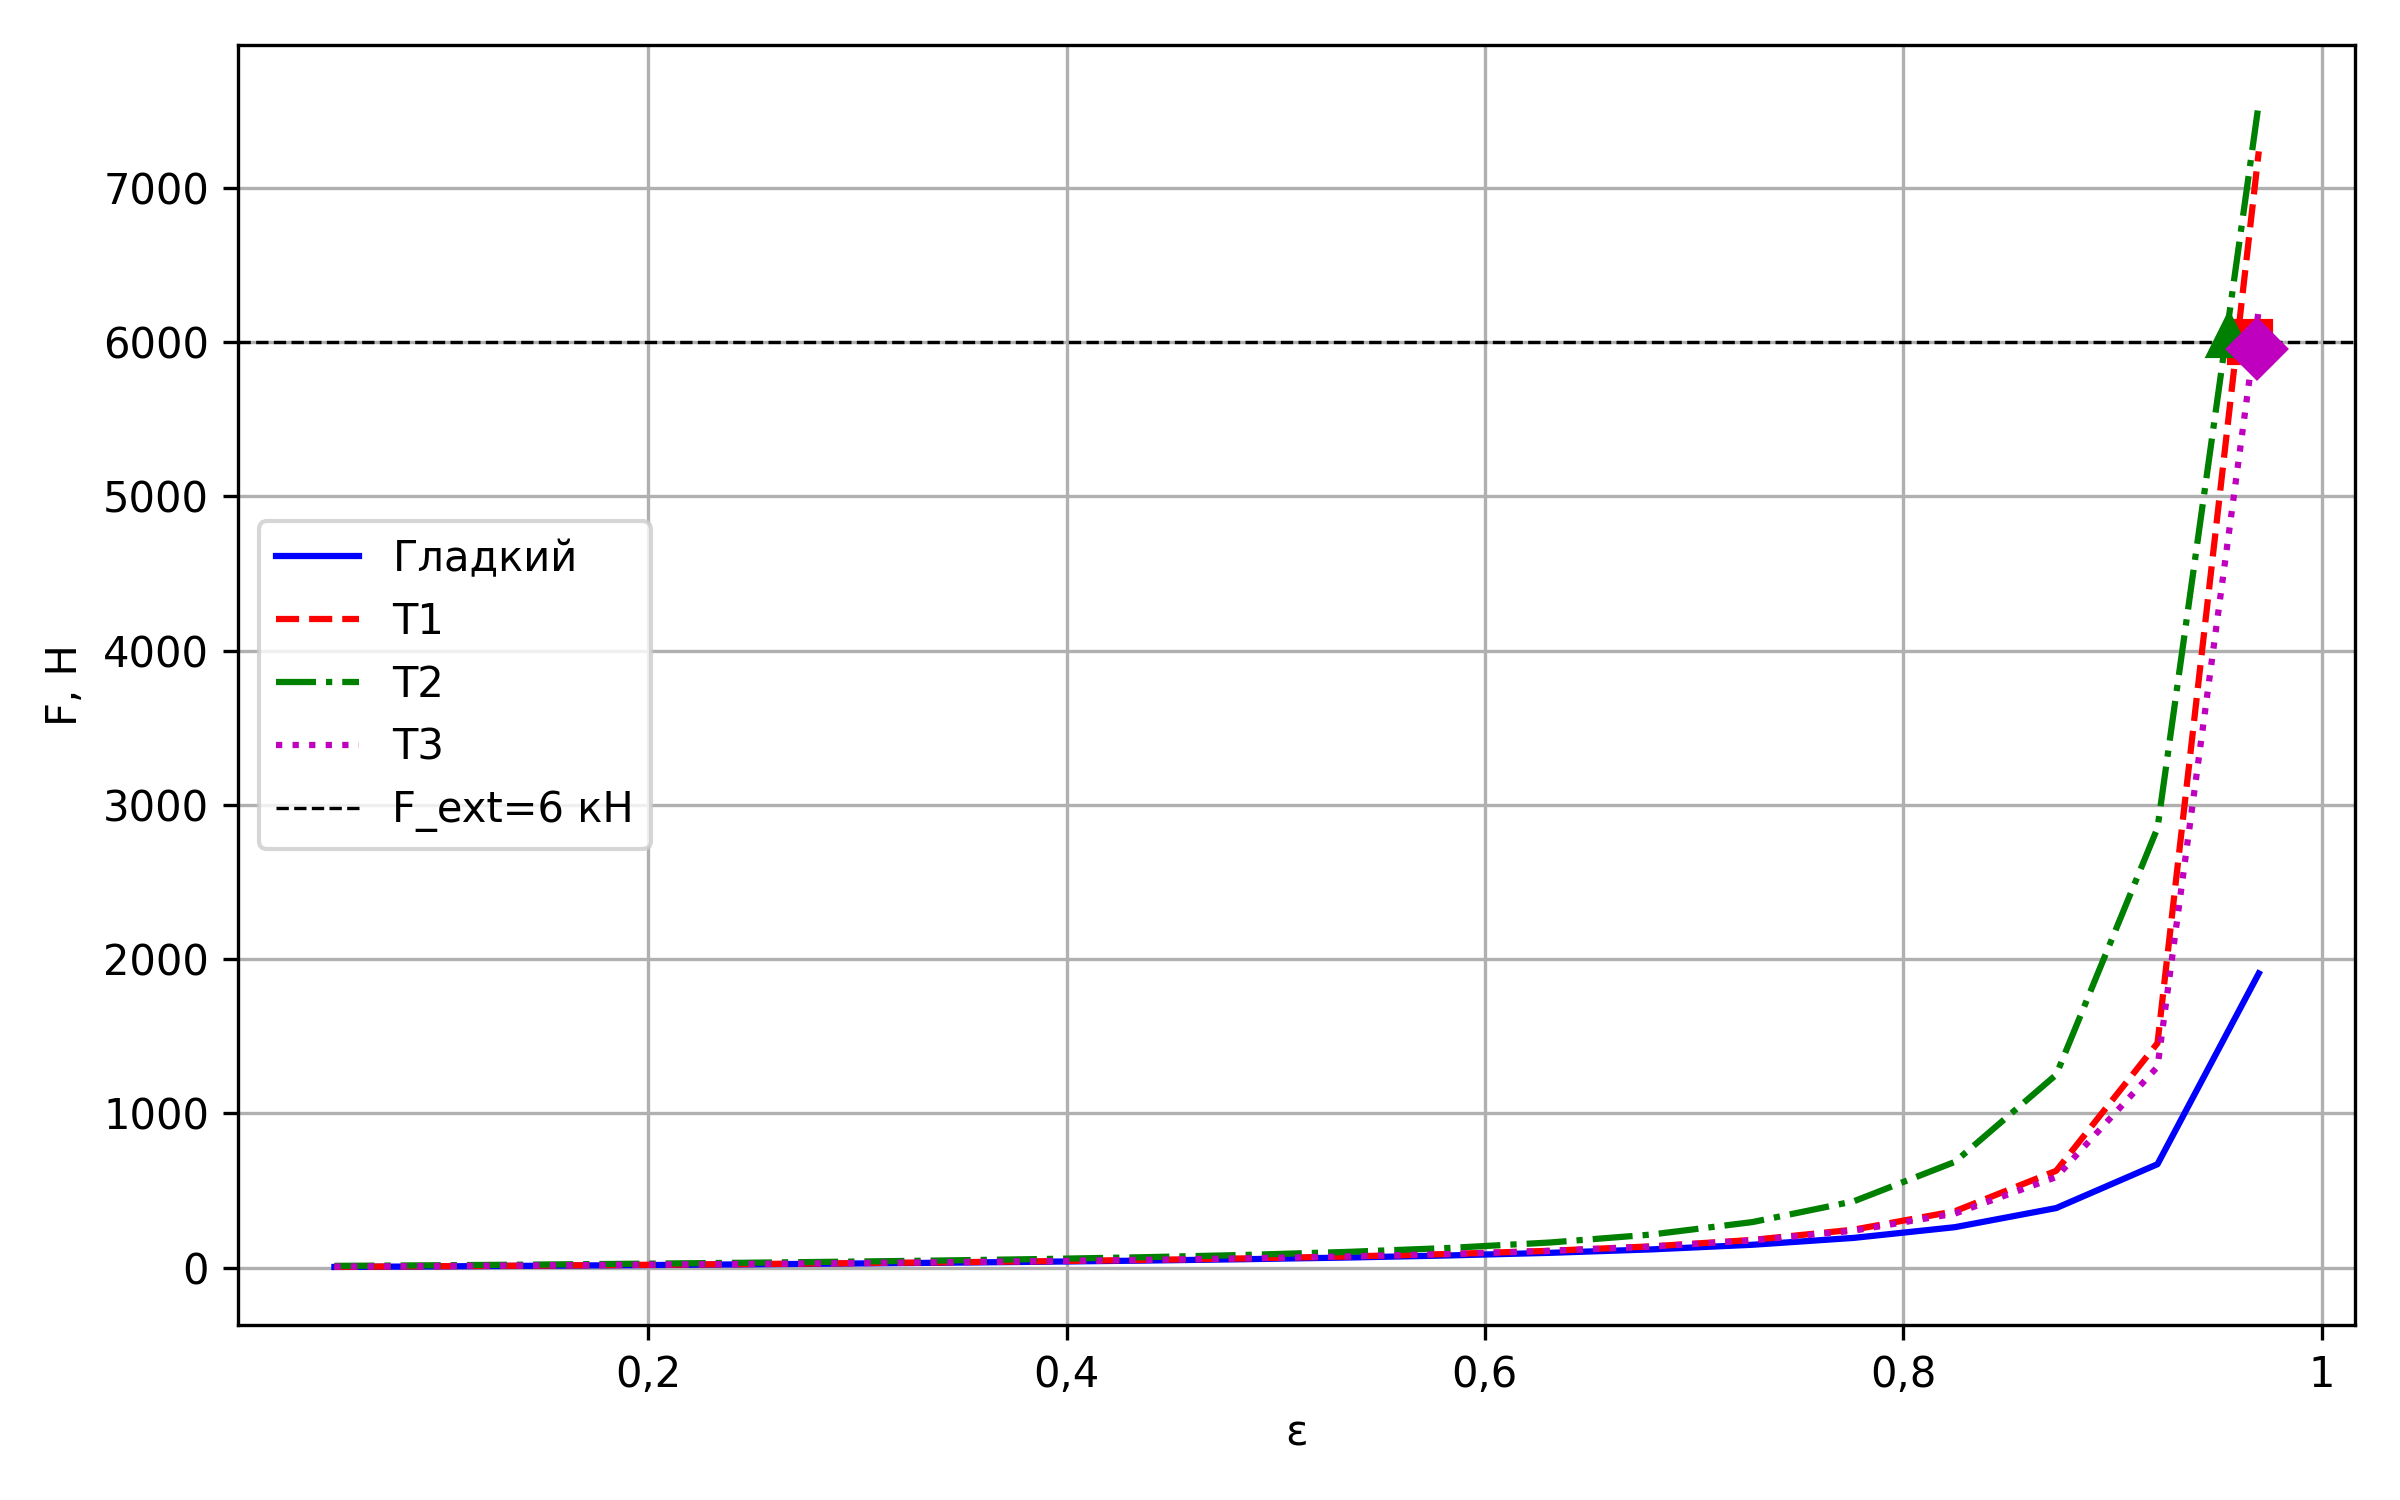
\includegraphics[width=\textwidth,height=0.9\textheight,keepaspectratio]{figures/ch06/fig_6_2.png}
\caption{Зависимость несущей силы $F$ от эксцентриситета $\varepsilon$
  для гладкого подшипника и конфигураций T1, T2, T3.
  Пунктирная горизонталь~-- рабочая нагрузка $F_{\mathrm{ext}} = 6\,000$~Н;
  маркеры~-- равновесные рабочие точки текстурированных конфигураций.}
\label{fig:bit_operating_points}
\end{figure}

\FloatBarrier

Параметр плёнки~$\lambda$ в рабочих точках текстурированных
конфигураций представлен на рисунке~\ref{fig:bit_lambda_comparison}.

\begin{figure}[!ht]
\centering
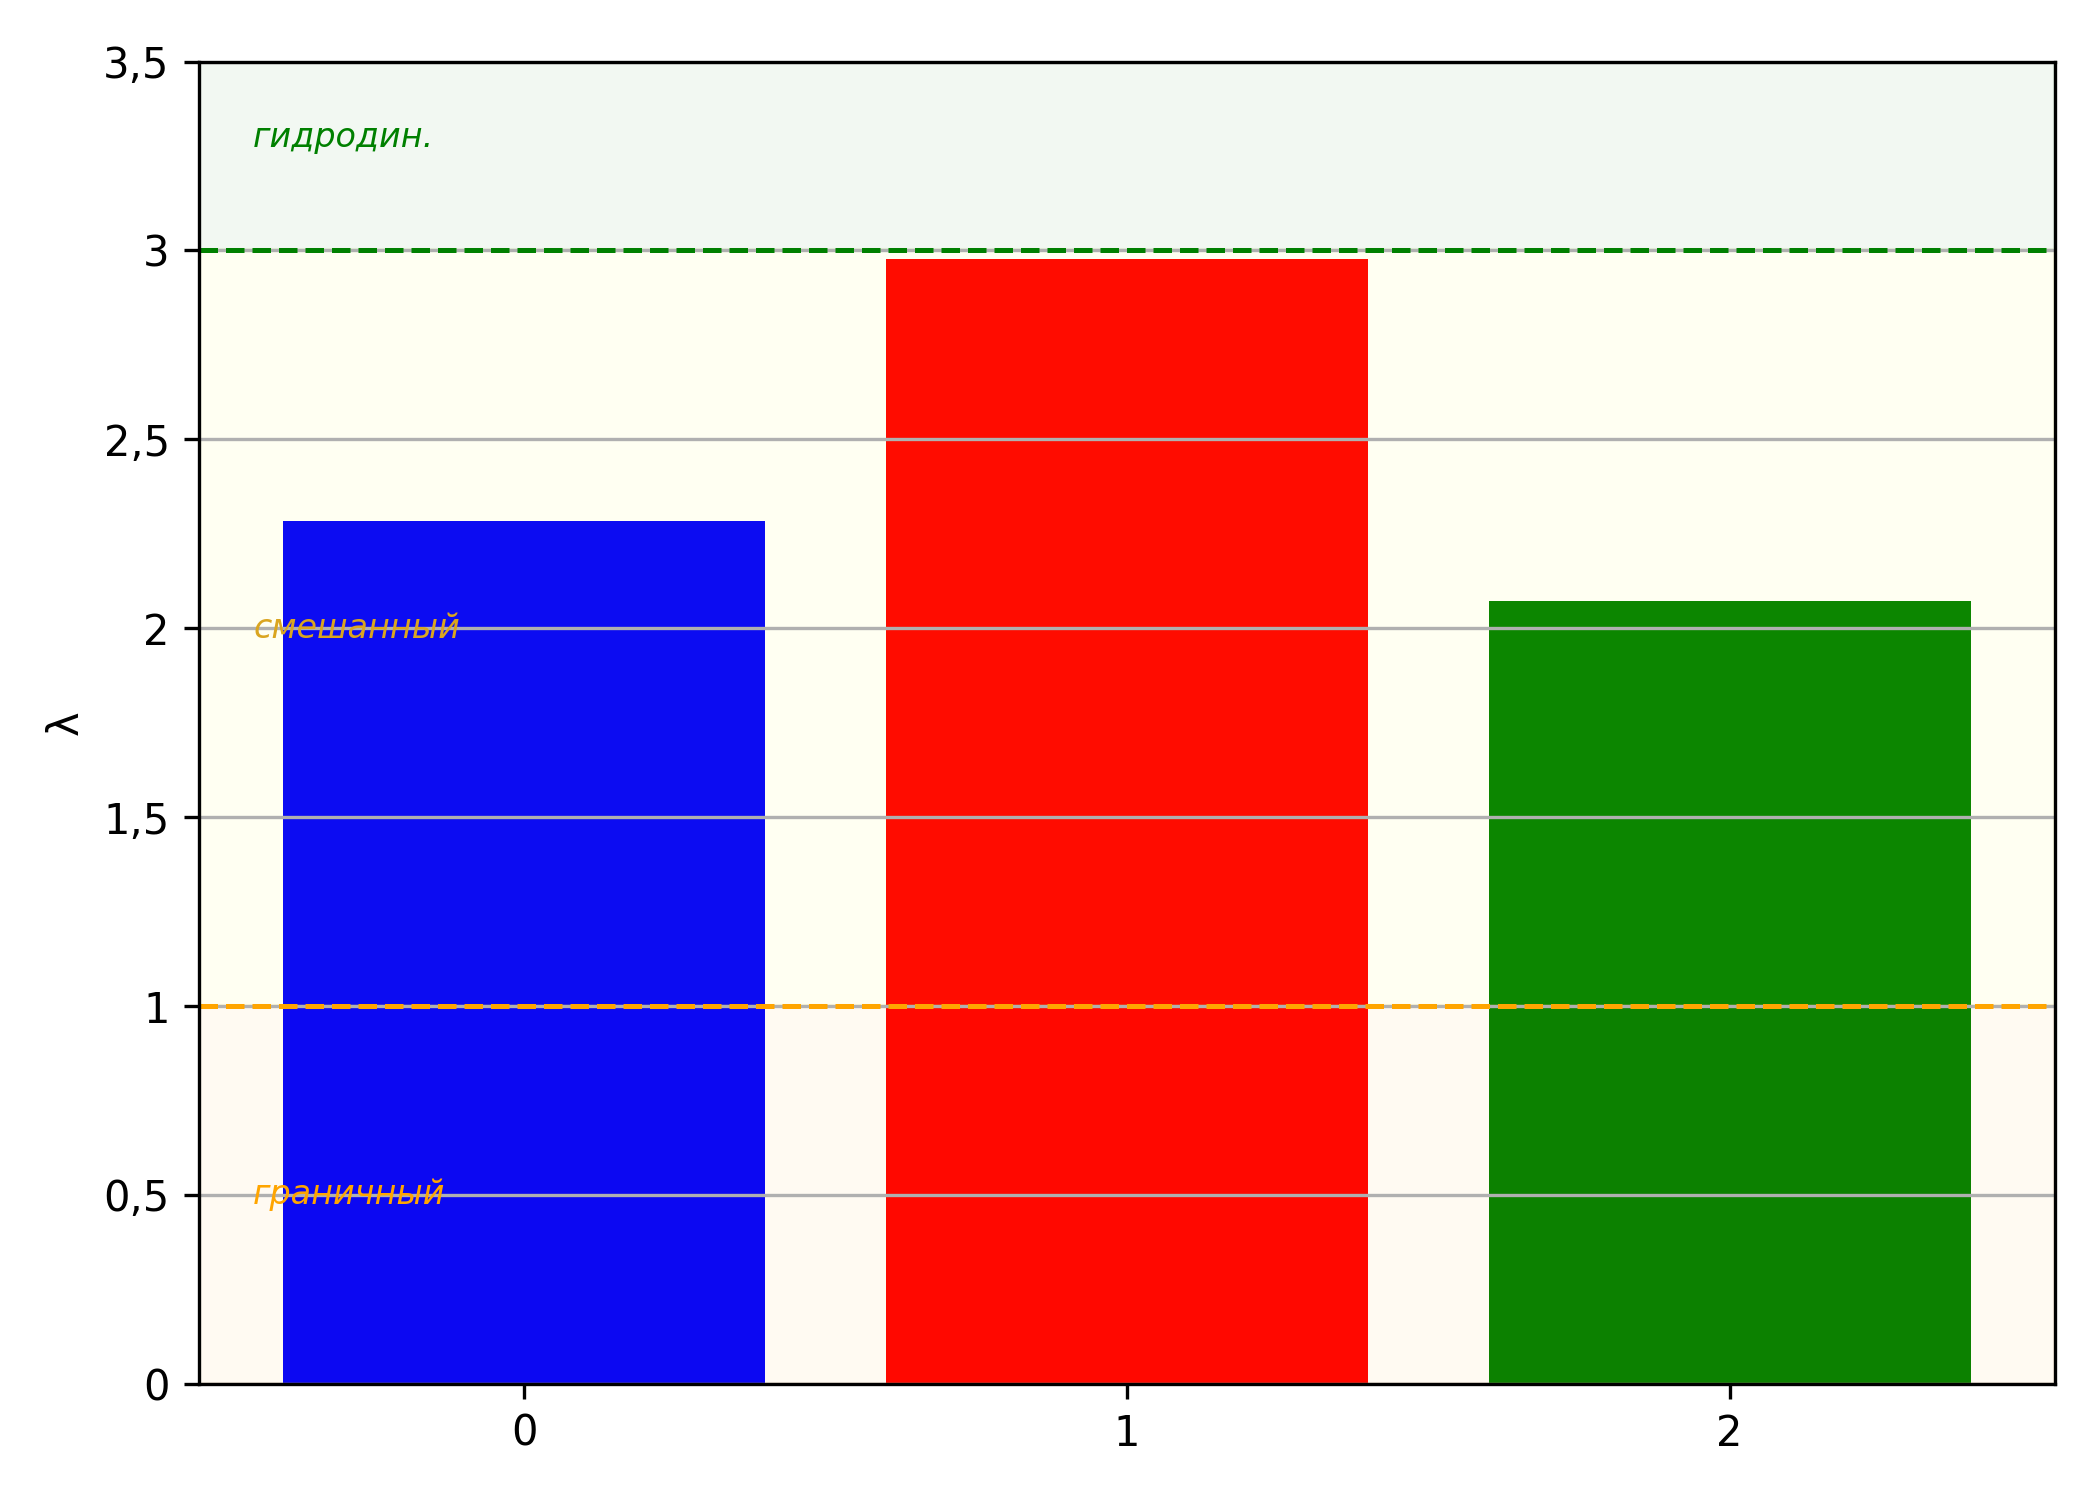
\includegraphics[width=\textwidth,height=0.9\textheight,keepaspectratio]{figures/ch06/fig_6_3.png}
\caption{Параметр плёнки $\lambda$ в рабочей точке ($F_{\mathrm{ext}} = 6\,000$~Н)
  для конфигураций T1, T2, T3. Пунктирные линии~-- границы режимов смазки:
  $\lambda = 1$ и $\lambda = 3$.}
\label{fig:bit_lambda_comparison}
\end{figure}

\FloatBarrier


\textit{Зависимости характеристик от нагрузки.}
Для оценки поведения подшипника при различных условиях нагружения
выполнен параметрический расчёт при~$F_{\mathrm{ext}}$ от
${\sim}\,2100$ до ${\sim}\,6800$~Н. Диапазон ограничен
грузоподъёмностью конфигураций при $\varepsilon = 0{,}97$.

С ростом нагрузки эксцентриситет монотонно возрастает
(рисунок~\ref{fig:bit_sweep_B_epsilon}). При одинаковой
нагрузке конфигурация~T2 имеет наименьший эксцентриситет,
T3~-- наибольший. Конфигурация~T3 достигает расчётного предела
при $F \approx 6200$~Н и теряет рабочую точку раньше, чем T1 и~T2.

\begin{figure}[!ht]
\centering
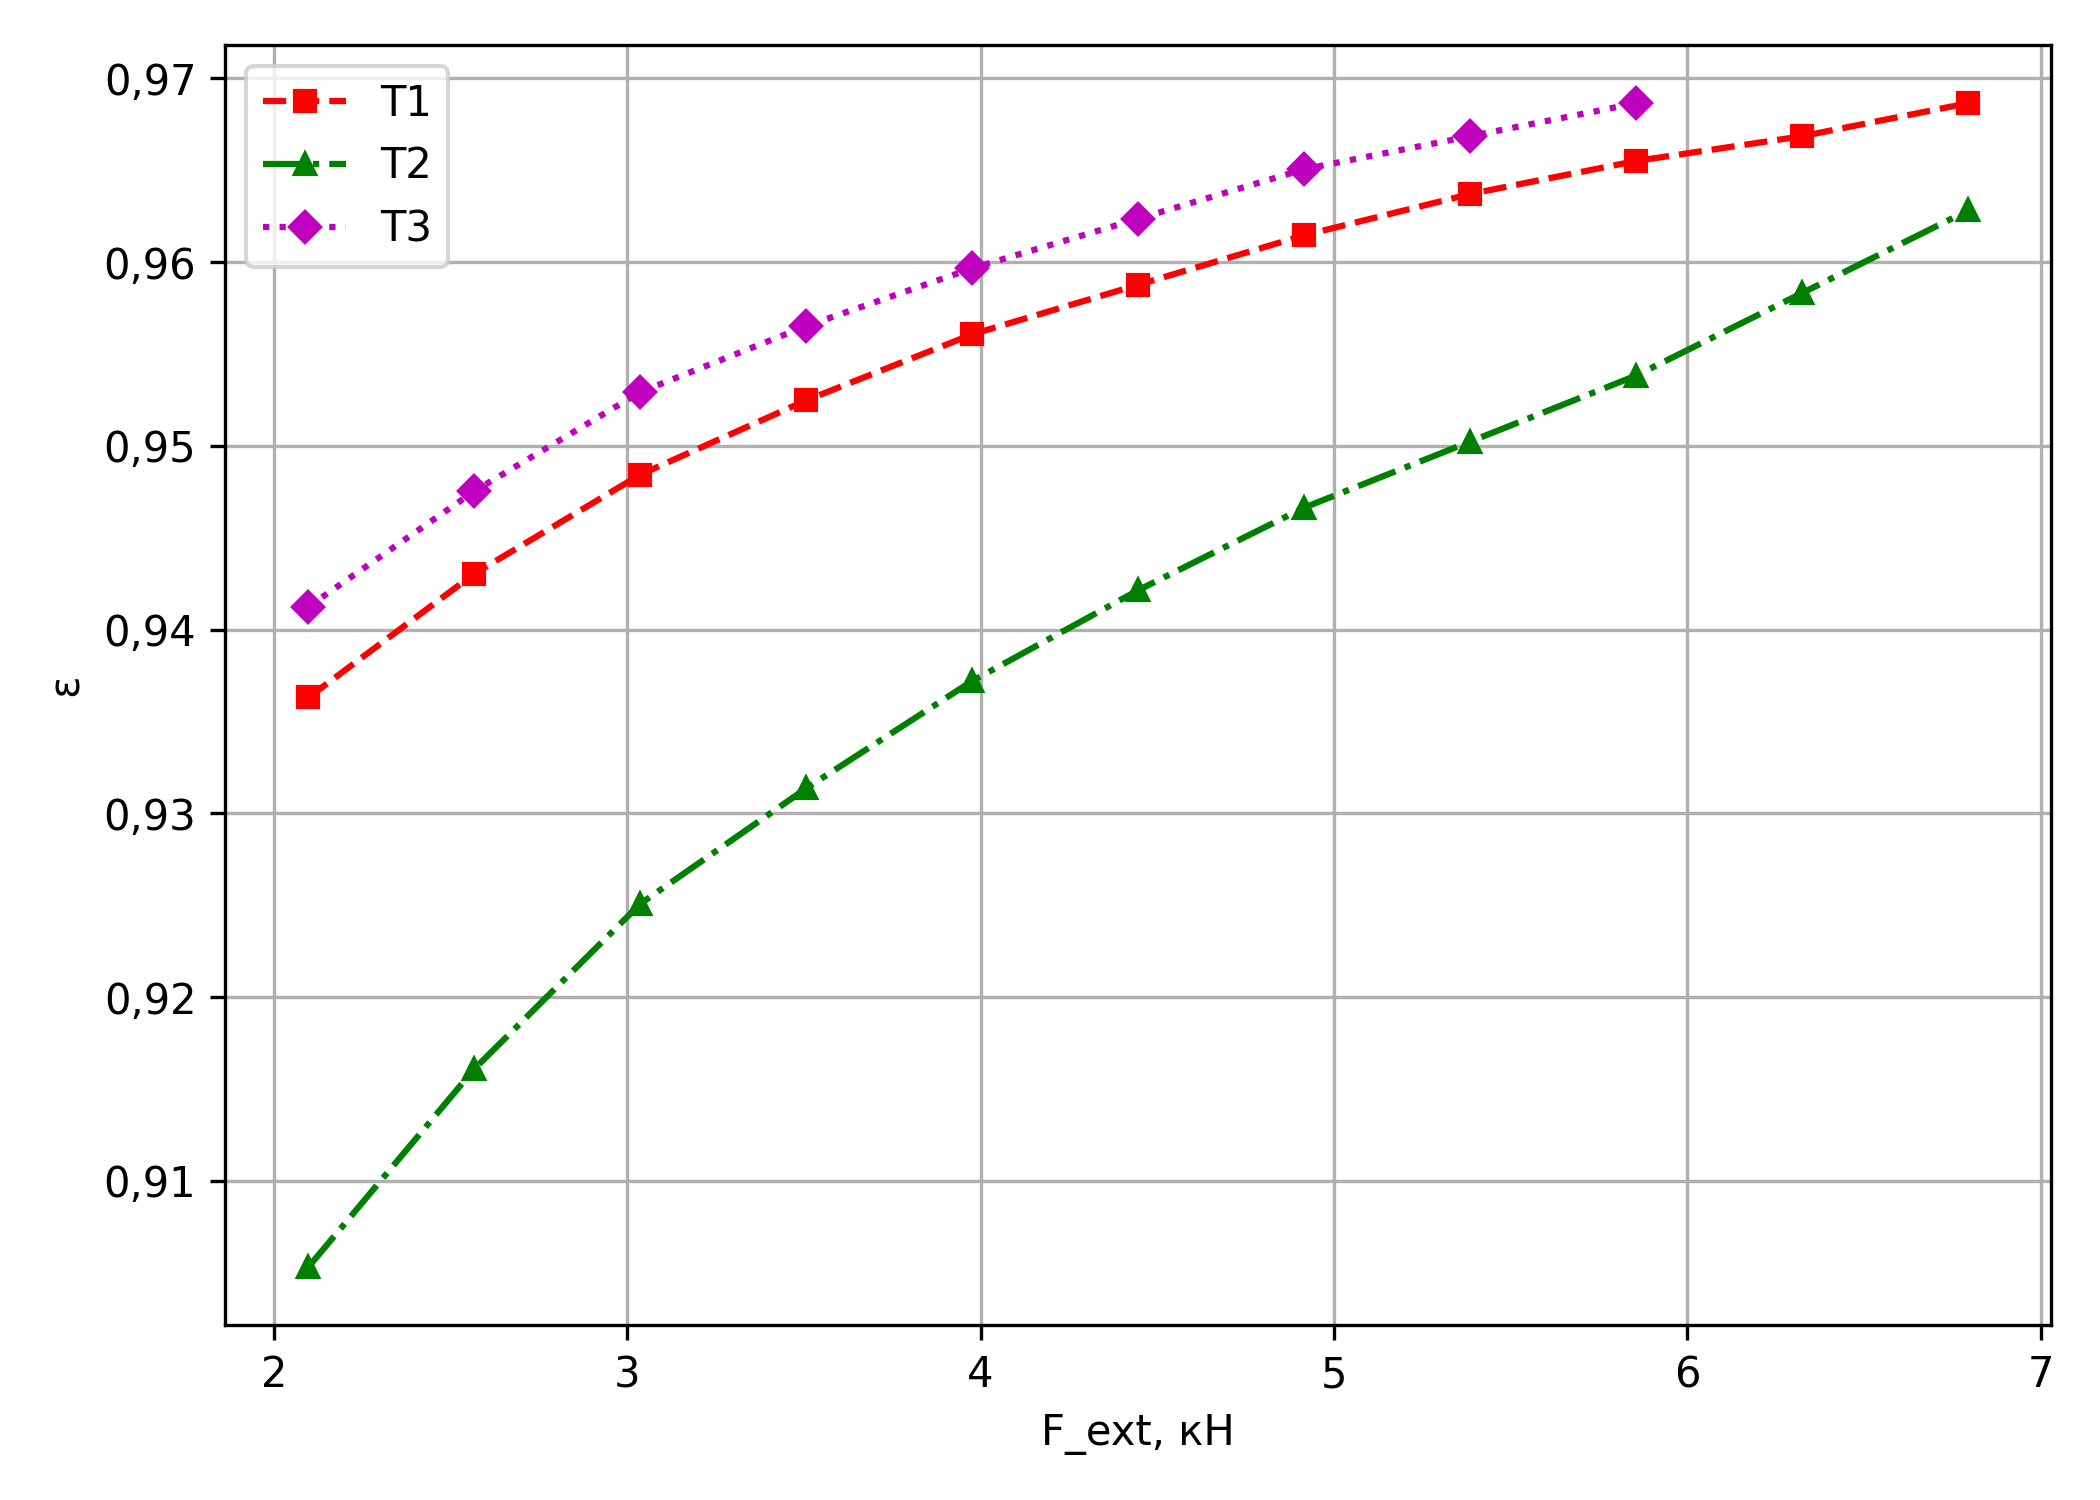
\includegraphics[width=\textwidth,height=0.9\textheight,keepaspectratio]{figures/ch06/fig_6_4.png}
\caption{Зависимость эксцентриситета $\varepsilon$ от нагрузки $F_{\mathrm{ext}}$
  для конфигураций T1, T2, T3 в рабочей зоне текстурированных вариантов.}
\label{fig:bit_sweep_B_epsilon}
\end{figure}

\FloatBarrier

Параметр плёнки~$\lambda$ убывает с ростом нагрузки
(рисунок~\ref{fig:bit_sweep_B_lambda}). При
$F \approx 6\,000$~Н конфигурация~T2 находится вблизи границы
смешанного и гидродинамического режимов ($\lambda \approx 3$);
конфигурации~T1 и~T3 остаются в смешанном режиме ($\lambda < 2{,}5$).

\begin{figure}[!ht]
\centering
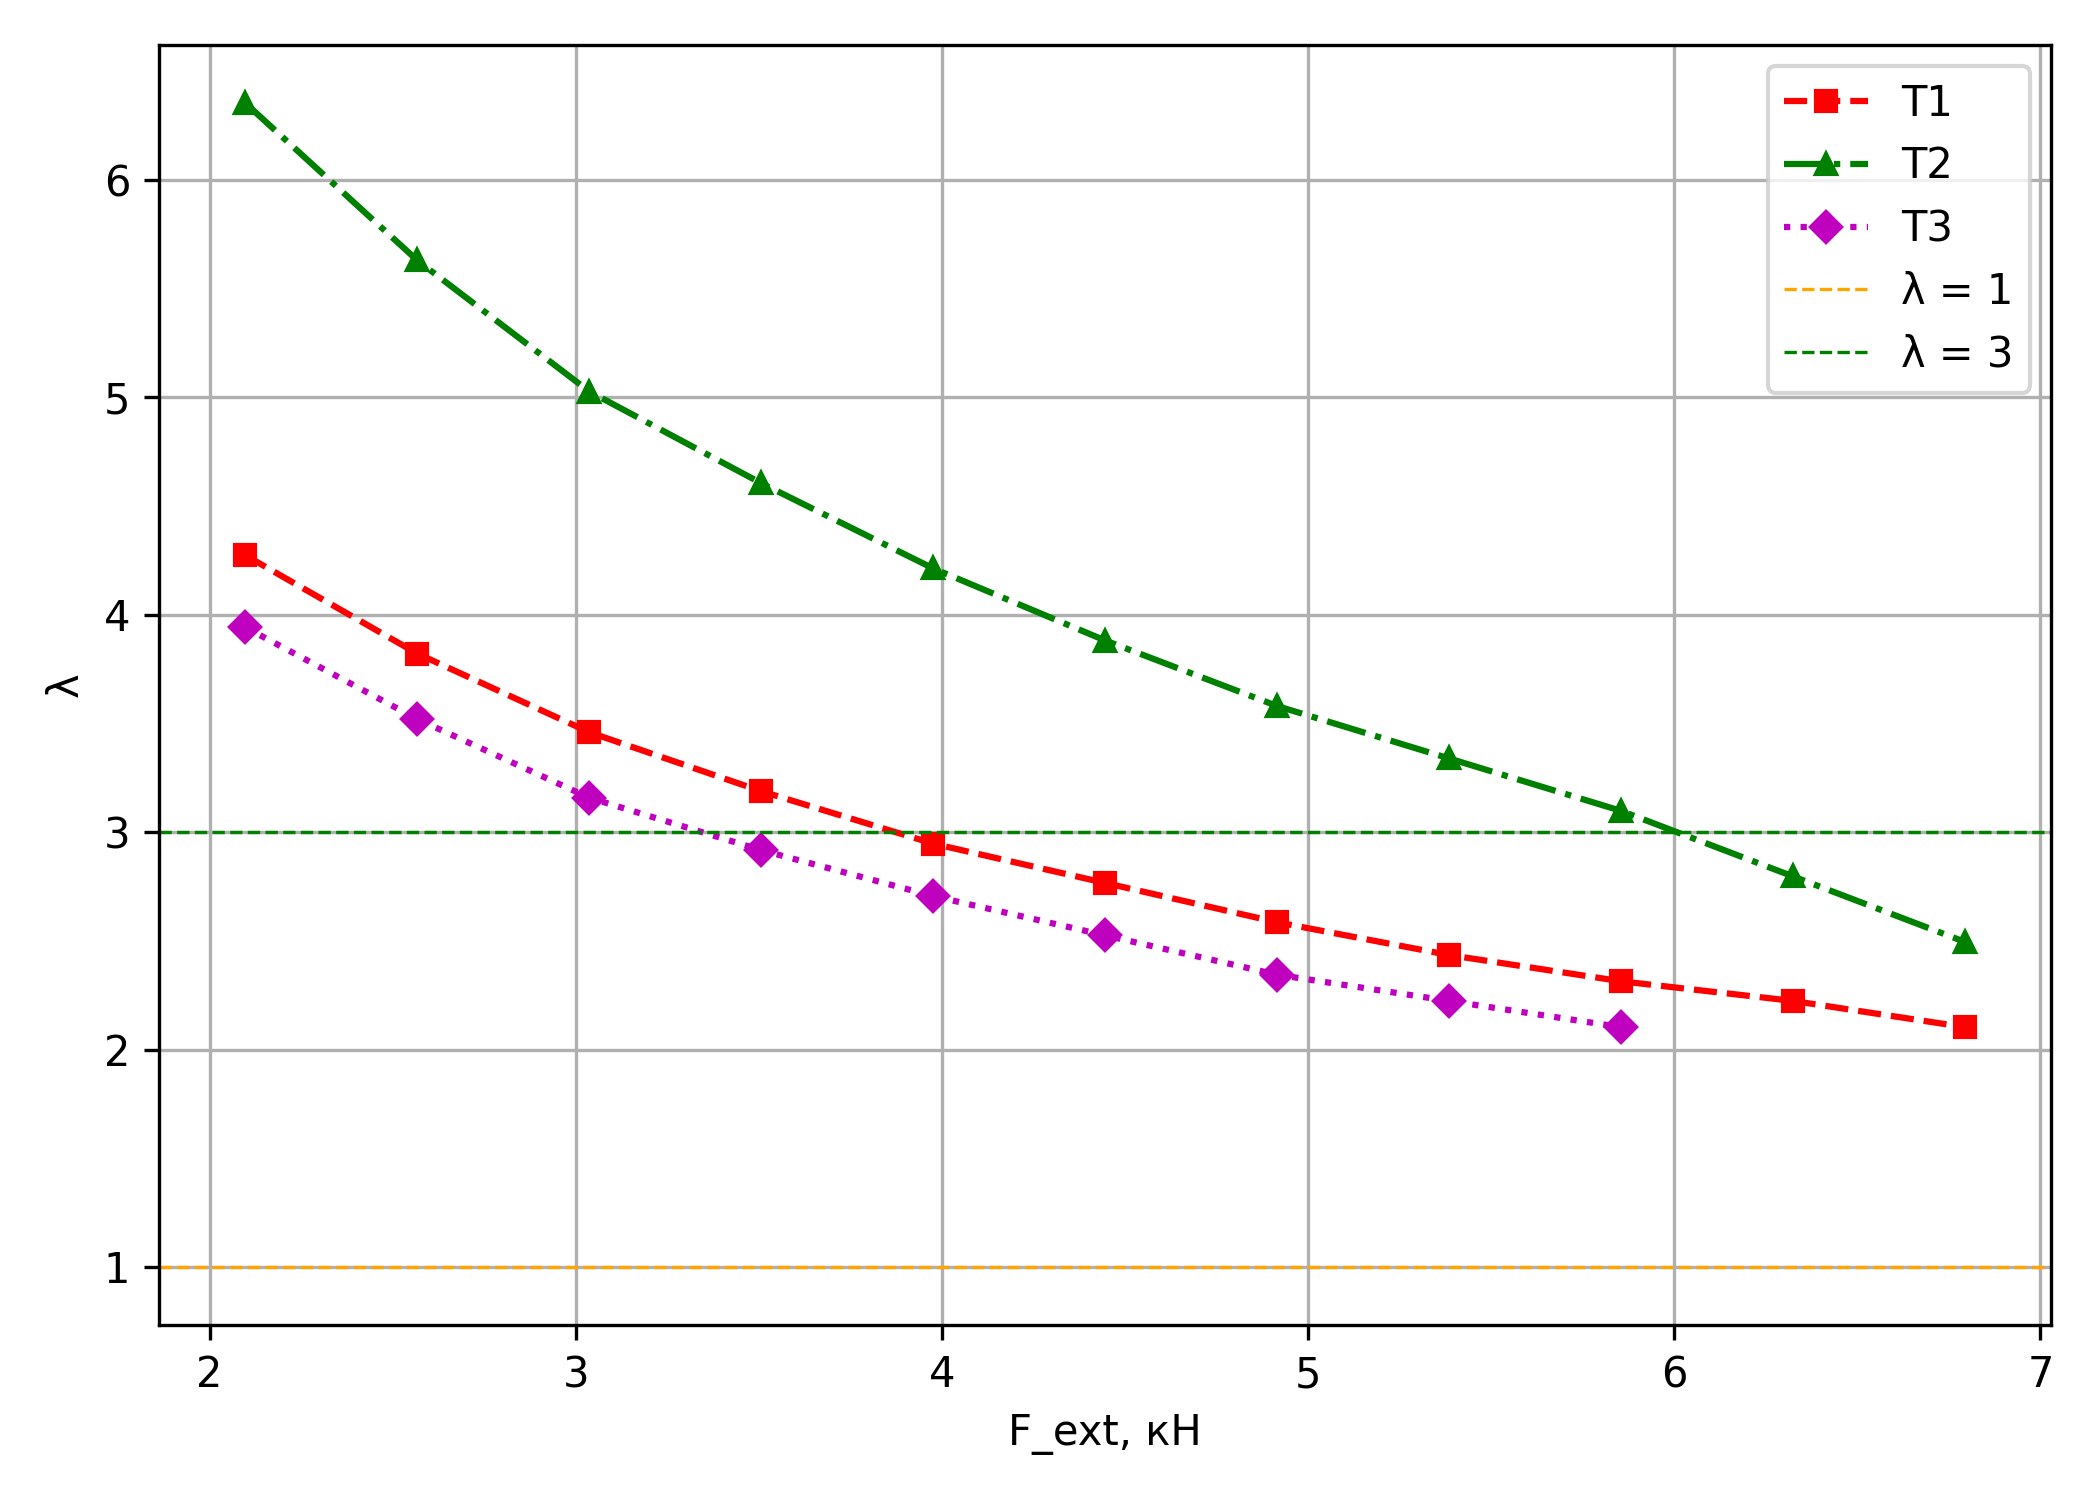
\includegraphics[width=\textwidth,height=0.9\textheight,keepaspectratio]{figures/ch06/fig_6_5.png}
\caption{Зависимость параметра плёнки $\lambda$ от нагрузки $F_{\mathrm{ext}}$.
  Пунктирные линии~-- границы режимов смазки $\lambda = 1$ и $\lambda = 3$.}
\label{fig:bit_sweep_B_lambda}
\end{figure}

\FloatBarrier

Минимальная толщина плёнки~$h_{\min}$ убывает с ростом нагрузки
(рисунок~\ref{fig:bit_sweep_B_hmin}). При $F = 6\,000$~Н:
$h_{\min} = 2{,}66$~мкм (T2), $2{,}04$~мкм (T1), $1{,}85$~мкм (T3),
что сопоставимо с суммарной шероховатостью
$\sigma_{\mathrm{eq}} = 0{,}89$~мкм.

\textit{Коэффициенты улучшения на общей достижимой нагрузке.}
При $F_{\mathrm{ext}} = 6\,000$~Н гладкий подшипник не имеет
рабочей точки, что исключает прямое нормирование характеристик
текстурированных вариантов на значения гладкого при рабочей нагрузке.
Нормированные показатели определяются при общей достижимой нагрузке:

\begin{figure}[!ht]
\centering
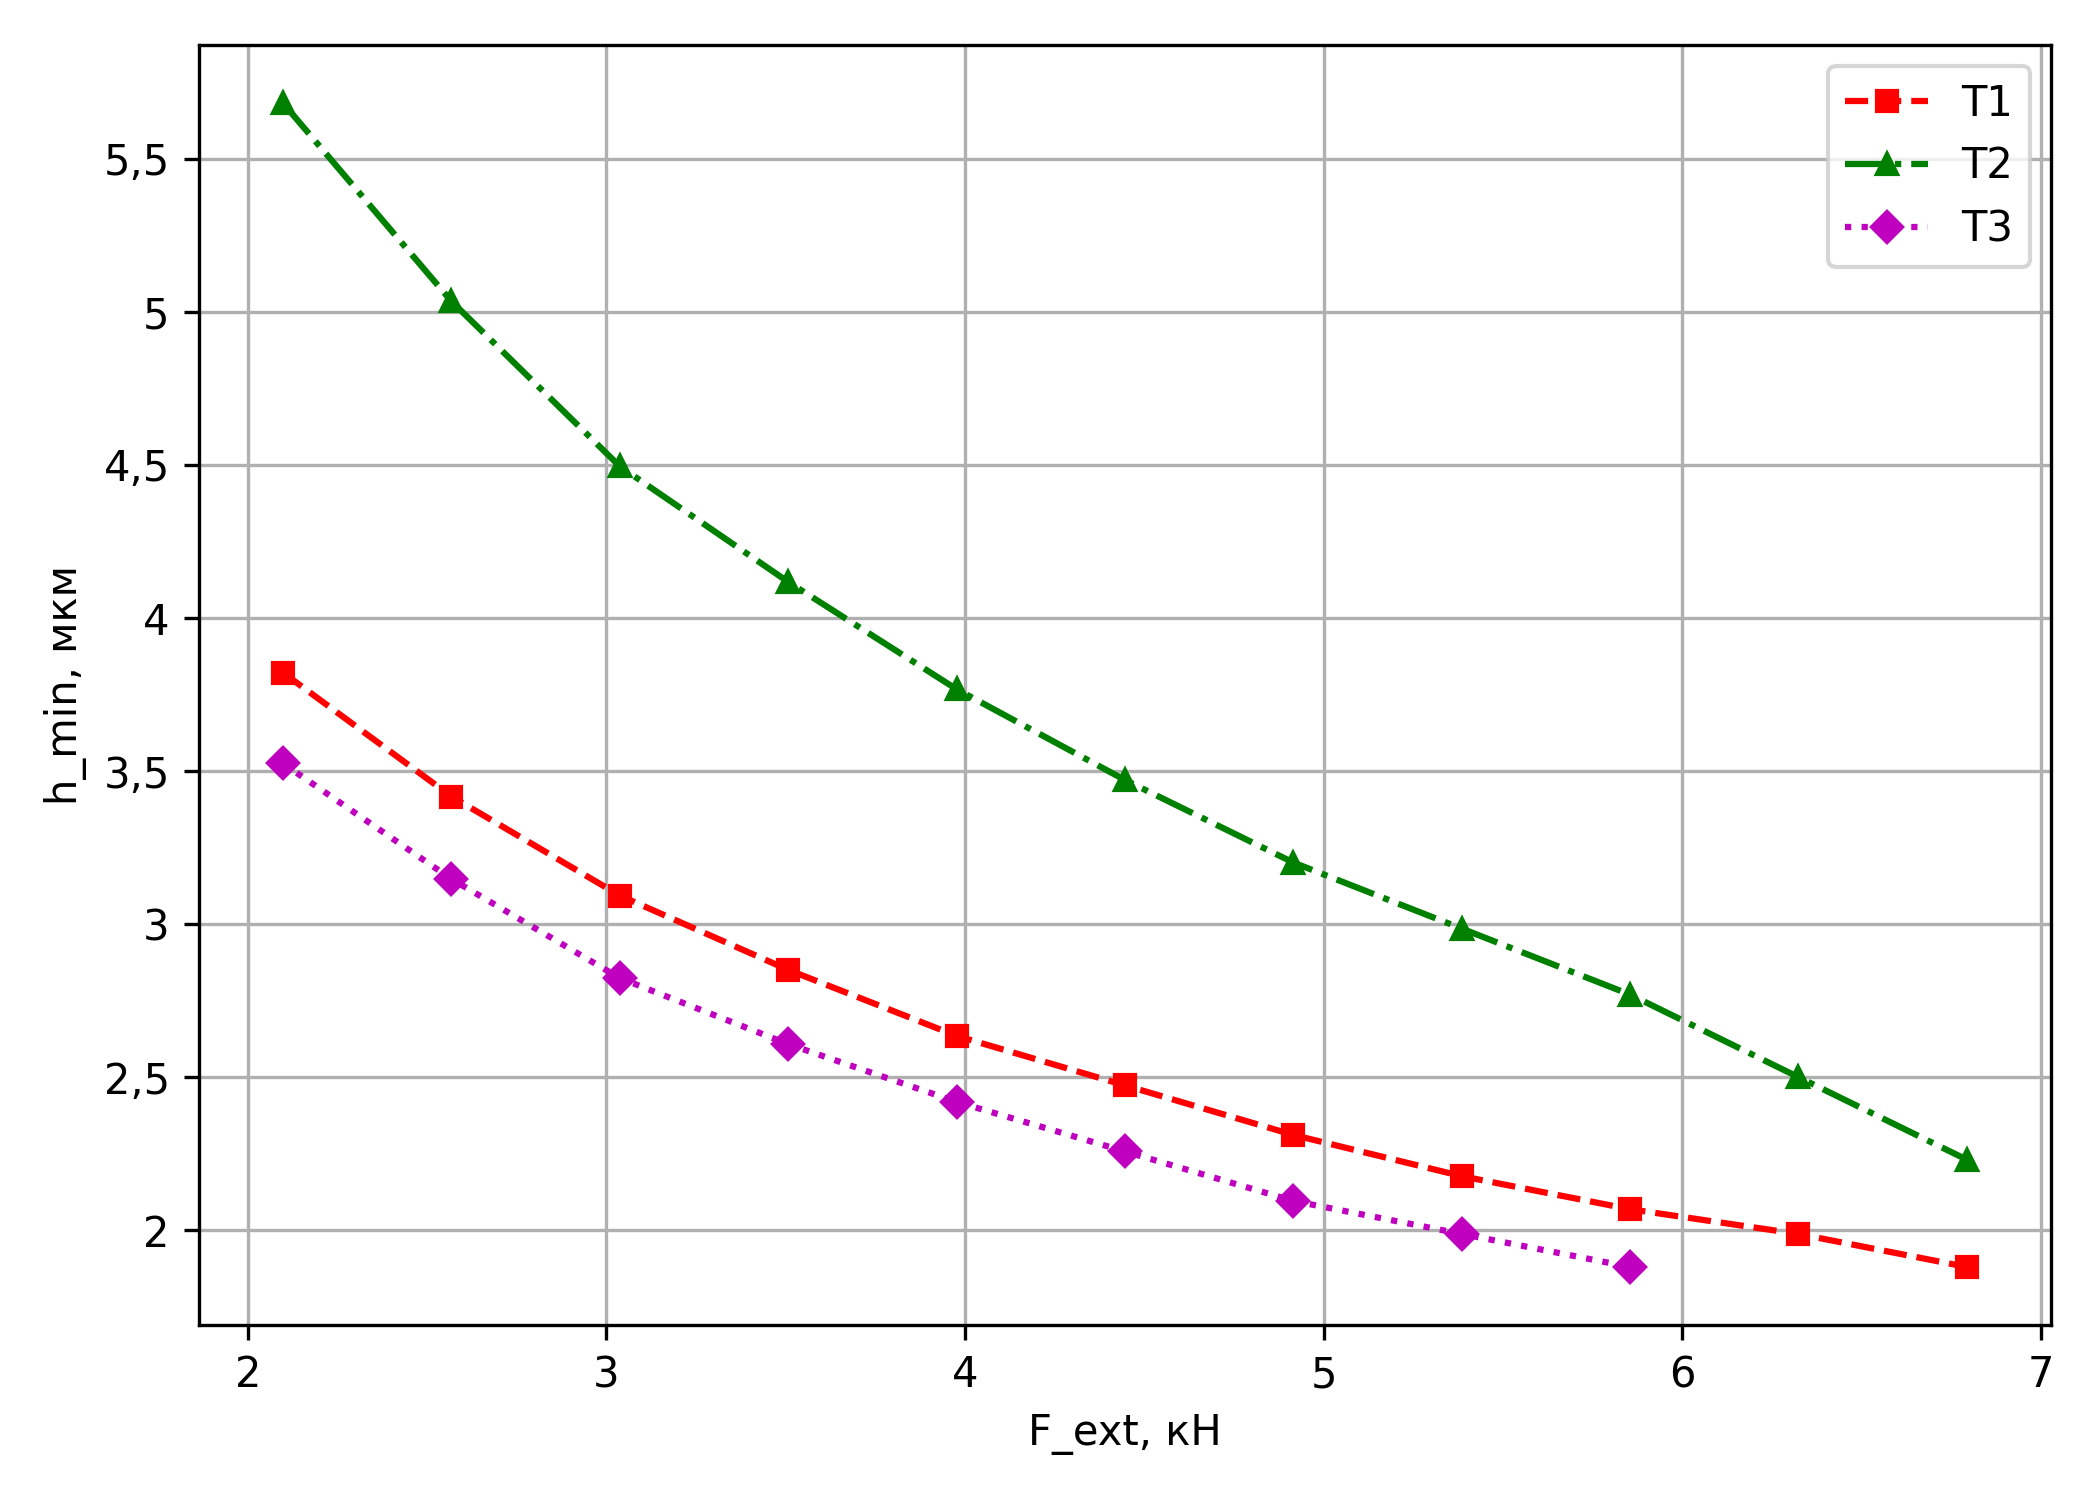
\includegraphics[width=\textwidth,height=0.9\textheight,keepaspectratio]{figures/ch06/fig_6_6.png}
\caption{Зависимость минимальной толщины плёнки $h_{\min}$ от нагрузки
  $F_{\mathrm{ext}}$ для конфигураций T1, T2, T3.}
\label{fig:bit_sweep_B_hmin}
\end{figure}
\begin{equation}
  F_* = 0{,}85 \cdot F_0
    (\varepsilon = 0{,}97) = 1\,621\;\text{Н},
  \label{eq:bit_Fcommon}
\end{equation}
при которой рабочая точка существует у всех вариантов, включая
гладкий.

Нормированные показатели эффективности определяются следующим
образом:
\begin{equation}
\begin{split}
  &G_{h}^{(i)} = \frac{h_{\min}^{(i)}}{h_{\min}^{(0)}},
  \quad
  G_{\lambda}^{(i)} = \frac{\lambda^{(i)}}{\lambda^{(0)}}, \\
  &G_{PV}^{(i)} = \frac{PV^{(0)}}{PV^{(i)}},
  \quad
  G_{w}^{(i)} = \frac{I_w^{(0)}}{I_w^{(i)}}.
\end{split}
  \label{eq:bit_gain_factors}
\end{equation}
где верхний индекс~$(0)$~-- гладкий вариант,
$(i)$~-- текстурированные конфигурации T1, T2, T3.
Значение~$G > 1$ желательно для всех четырёх показателей.

Результаты расчёта нормированных показателей при
$F_* = 1\,621$~Н сведены в
таблицу~\ref{tab:bit_gains}.

\begin{table}[!ht]
\centering
\caption{Нормированные показатели эффективности при
  $F_* = 1\,621$~Н}
\label{tab:bit_gains}
\begin{tabularx}{\textwidth}{|X|c|c|c|c|}
\hline
\multicolumn{1}{|c|}{\textbf{Конфигурация}}
  & $\boldsymbol{G_h}$
  & $\boldsymbol{G_{\lambda}}$
  & $\boldsymbol{G_{PV}}$
  & $\boldsymbol{G_w}$ \\
\hline
T1 & 2{,}119 & 2{,}119 & 1{,}009 & 2{,}137 \\
\hline
T2 & 3{,}147 & 3{,}147 & 1{,}002 & 3{,}153 \\
\hline
T3 & 1{,}964 & 1{,}964 & 0{,}996 & 1{,}956 \\
\hline
\end{tabularx}
\end{table}

\FloatBarrier

Конфигурация~T2 обеспечивает $G_h = 3{,}147$
и $G_{\lambda} = 3{,}147$~-- утроение минимального зазора
и параметра плёнки по сравнению с гладким подшипником.
Показатель~$G_{PV}$ у всех конфигураций близок к единице:
при фиксированной нагрузке номинальное давление~$p_0$
практически не изменяется, и основной эффект текстурирования
реализуется через снижение эксцентриситета и рост зазора,
а не через изменение~$PV$. У конфигурации~T3
$G_{PV} = 0{,}996 < 1$~-- незначительный рост~$PV$, согласующийся
с меньшей несущей способностью этой конфигурации.

Нормированные показатели наглядно сопоставлены на
рисунке~\ref{fig:bit_gains_common}.

\begin{figure}[!ht]
\centering
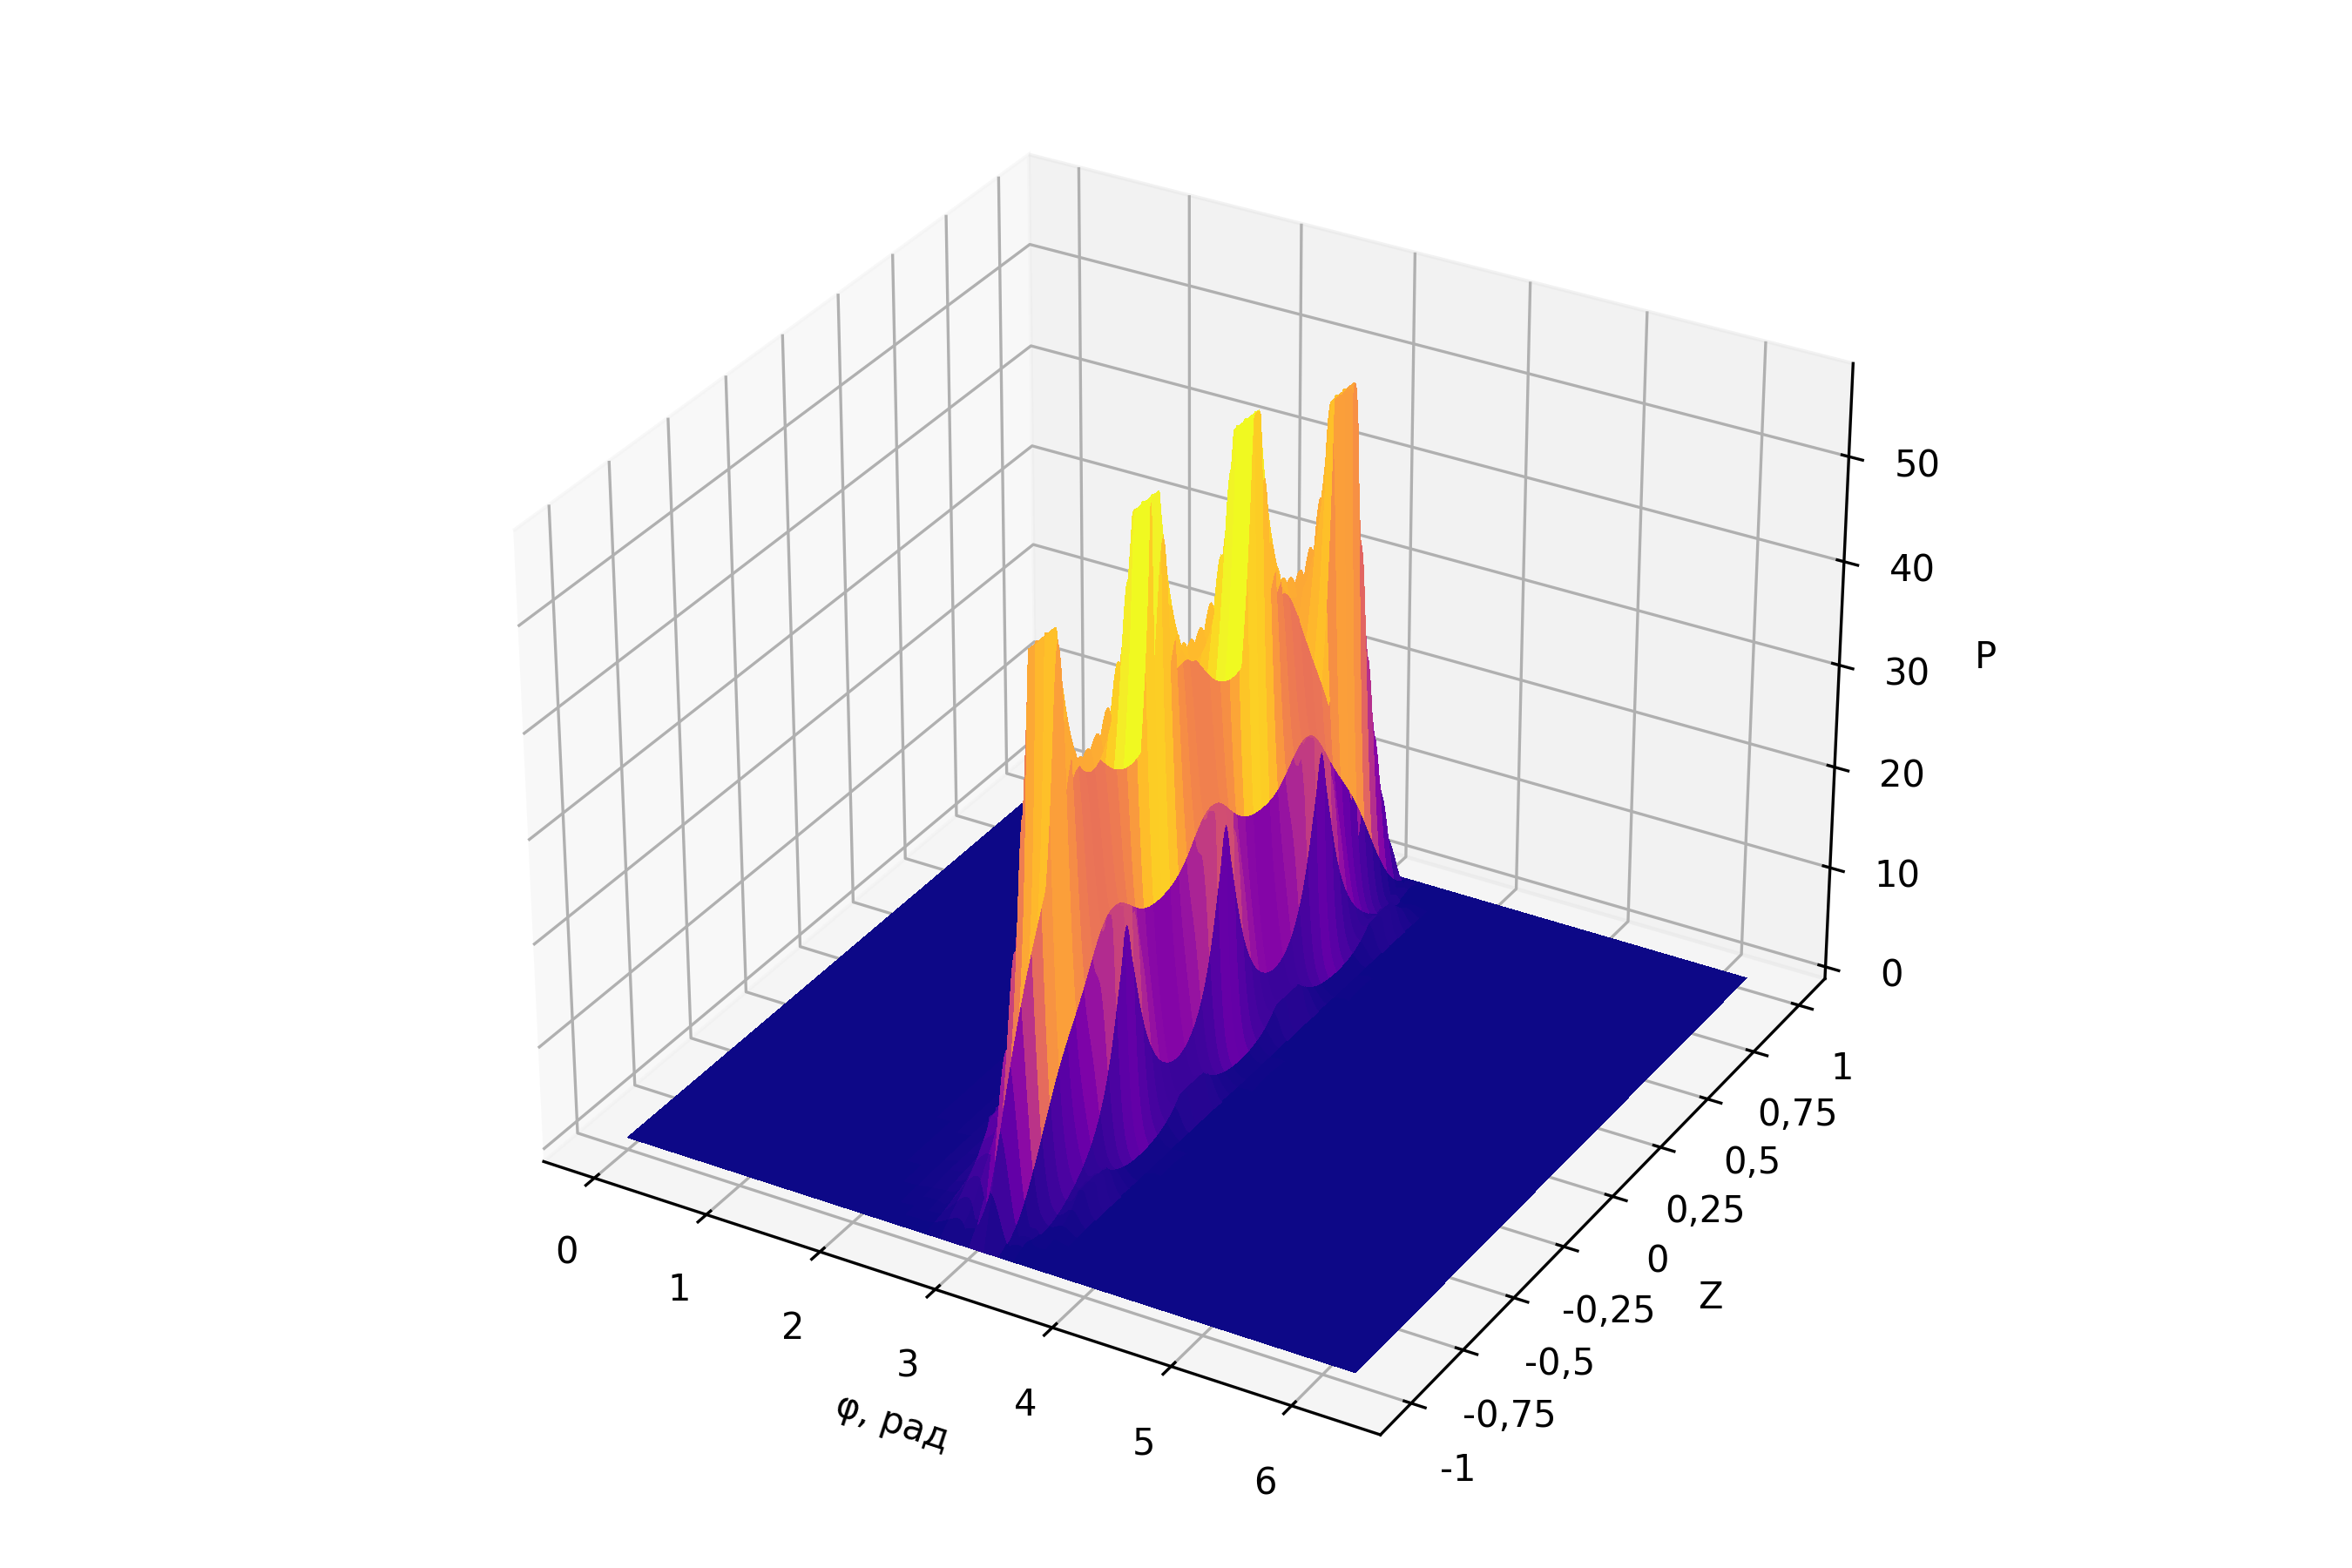
\includegraphics[width=\textwidth,height=0.9\textheight,keepaspectratio]{figures/ch06/fig_6_7.png}
\caption{Нормированные показатели эффективности $G_h$, $G_{\lambda}$,
  $G_{PV}$, $G_w$ для конфигураций T1, T2, T3
  при $F_* = 1\,621$~Н.
  Пунктирная горизонталь $G = 1$~-- уровень гладкого подшипника.}
\label{fig:bit_gains_common}
\end{figure}

\FloatBarrier


\textit{Поле давления лучшей конфигурации.}
Для конфигурации~T2, продемонстрировавшей наилучшие характеристики,
представлено трёхмерное поле безразмерного давления~$P(\theta, Z)$
в рабочей точке ($\varepsilon = 0{,}956$). Зона максимального
давления располагается вблизи $\theta \approx \pi$. Лунки
конфигурации~T2 формируют выраженную <<рябь>> на поверхности
давления, свидетельствующую о локальном перераспределении потоков
в каждом элементе микрорельефа
(рисунок~\ref{fig:bit_P3D_T2}).

\begin{figure}[!ht]
\centering
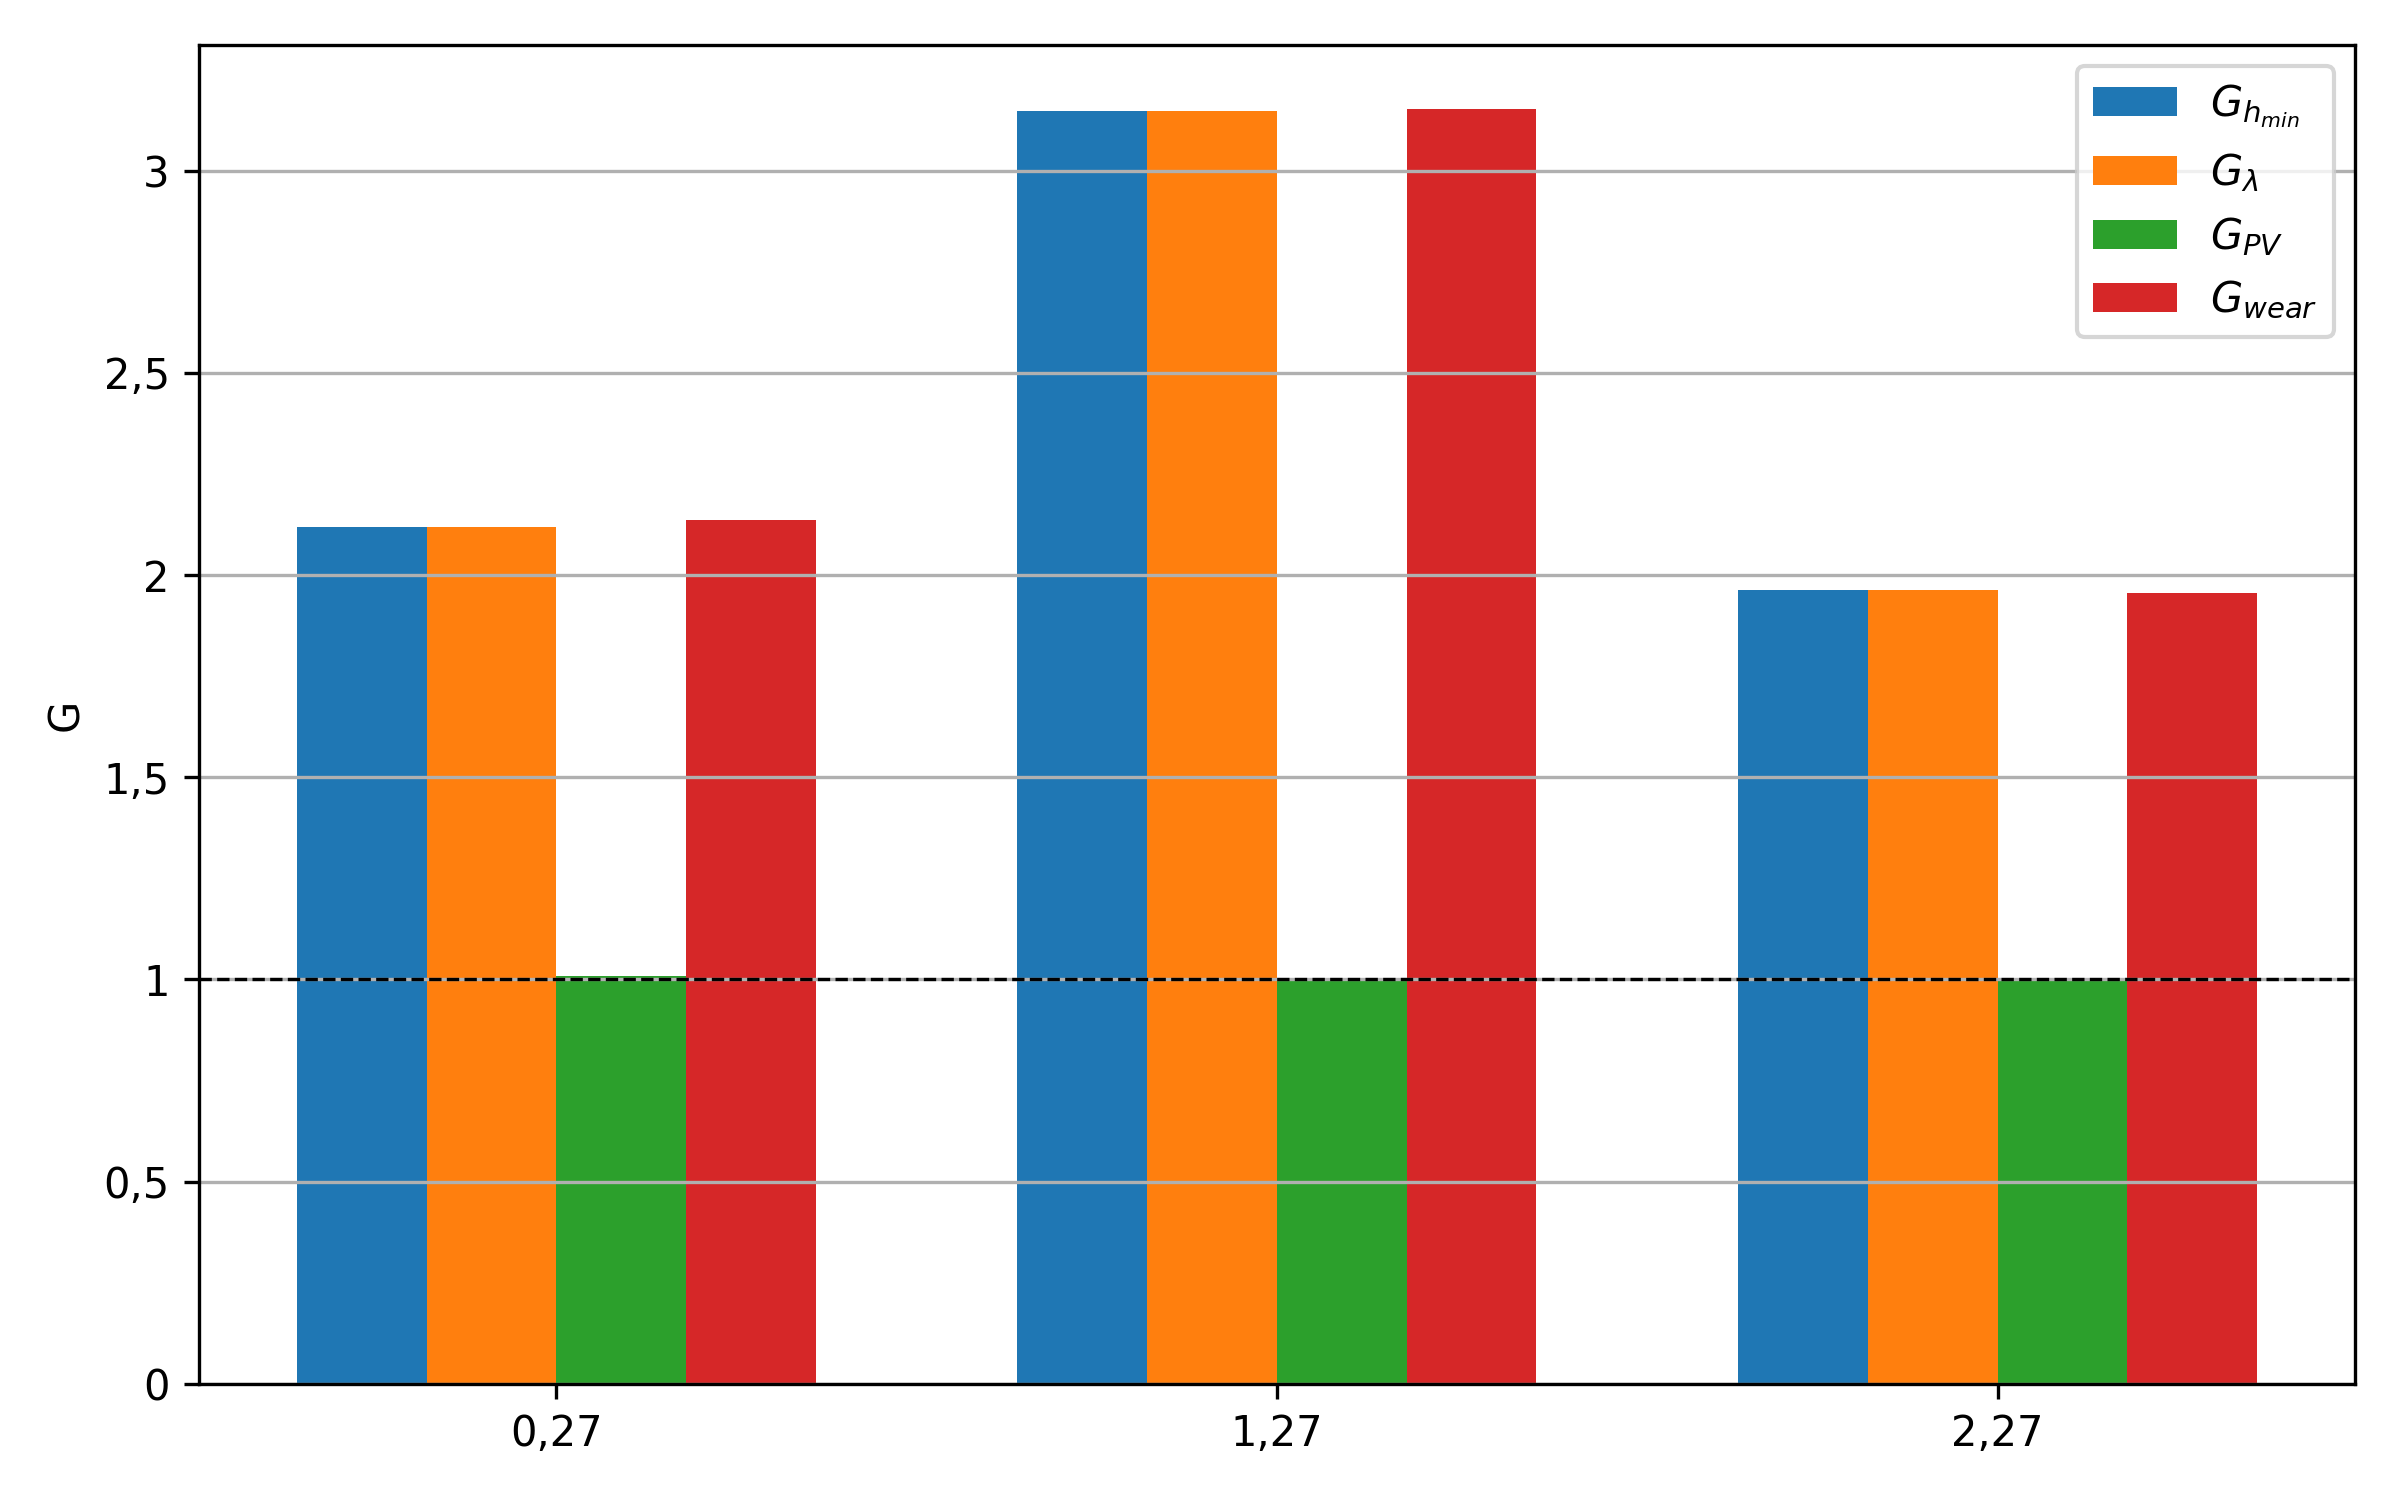
\includegraphics[width=\textwidth,height=0.9\textheight,keepaspectratio]{figures/ch06/fig_6_8.png}
\caption{Поле безразмерного давления $P(\theta, Z)$
  для конфигурации~T2 ($H_p = 0{,}40$, зона $90^{\circ}$--$270^{\circ}$)
  в рабочей точке $\varepsilon = 0{,}956$.}
\label{fig:bit_P3D_T2}
\end{figure}


\FloatBarrier
\section*{Выводы по главе~6}
\phantomsection\addcontentsline{toc}{section}{Выводы по главе~6}

Проведён анализ радиального подшипника скольжения опоры шарошки
трёхшарошечного долота в изотермическом приближении с учётом
кавитации по условию Рейнольдса ($P \geq 0$). Установлено, что
гладкий подшипник при рабочей нагрузке
$F_{\mathrm{ext}} = 6\,000$~Н не имеет равновесной рабочей точки
в чисто гидродинамической постановке:
$F(\varepsilon = 0{,}97) = 1907$~Н.

Текстурирование поверхности цапфы эллипсоидальными лунками
в шахматной раскладке существенно повышает гидродинамическую
несущую способность: $F(\varepsilon = 0{,}97)$ достигает
$7549$~Н (конфигурация~T2), что в~$3{,}96$ раза превышает
значение гладкого варианта. Рабочая точка при
$F_{\mathrm{ext}} = 6\,000$~Н найдена для всех конфигураций
T1--T3.

В рабочих точках все конфигурации функционируют в смешанном режиме
смазки ($\lambda \approx 2{,}1$--$3{,}0$). Конфигурация~T2
($H_p = 0{,}40$, зона $90^{\circ}$--$270^{\circ}$) демонстрирует
наилучшие показатели: $\varepsilon = 0{,}956$,
$h_{\min} = 2{,}66$~мкм, $\lambda = 2{,}98$~-- значение,
наиболее близкое к границе гидродинамического режима.

На общей достижимой нагрузке $F_* = 1\,621$~Н
конфигурация~T2 обеспечивает трёхкратное увеличение минимального
зазора ($G_h = 3{,}15$) и параметра плёнки
($G_{\lambda} = 3{,}15$). Показатели~$G_{PV}$ близки к единице
(фиксированная нагрузка); основной эффект текстурирования
реализуется через рост минимального зазора и улучшение условий
смазки.

Анализ упорного подшипника скольжения с детерминированными
микроструктурами выполнен в главе~7.



\section{Пример анализа упорного подшипника скольжения}

Третий пример демонстрирует расчёт упорного подшипника скольжения с~секторными колодками. В~отличие от~радиальных подшипников, рассмотренных выше, несущая способность упорного подшипника обусловлена клиновым зазором между колодкой и~диском, а~задача формулируется в~цилиндрических координатах. Пример позволяет студенту освоить постановку задачи и~методику расчёта для~принципиально иного типа подшипника.

% =============================================================
% 7 Анализ упорного подшипника скольжения
% =============================================================
\chapter{Анализ рельефного упорного подшипника скольжения}

\section{Объект исследования и исходные данные}

Объектом исследования в настоящей главе является упорный подшипник
скольжения с секторными колодками~\cite{gropper2018,wasilczuk2008}. Неподвижные колодки удерживают
осевую нагрузку вращающегося диска (ротора). Подшипник состоит
из~$N_{\mathrm{pads}} = 6$ одинаковых секторных колодок; расчёт
ведётся для одного сектора с последующим пересчётом интегральных
характеристик на полный подшипник.

В отличие от радиального подшипника (главы~5 и~6), где несущая сила
обусловлена эксцентриситетом цапфы, в упорном подшипнике давление
возникает вследствие клинового зазора между колодкой и диском.
Основным геометрическим параметром является параметр клина
$K = h_{\mathrm{in}} / h_{\mathrm{out}}$, где
$h_{\mathrm{in}}$~-- зазор на входной кромке сектора,
$h_{\mathrm{out}}$~-- зазор на выходной кромке.
Характер уравнения Рейнольдса также отличается: задача формулируется
в цилиндрических координатах $(r, \theta)$, а скорость скольжения
зависит от радиуса: $U(r) = \omega \cdot r$~\cite{brajdic2005,heinrichson2008}.

Основные параметры подшипника сведены в
таблицу~\ref{tab:thrust_params}.

\begin{table}[!ht]
\centering
\caption{Параметры упорного подшипника скольжения}
\label{tab:thrust_params}
\begin{tabularx}{\textwidth}{|X|c|c|c|}
\hline
\multicolumn{1}{|c|}{\textbf{Параметр}} & \textbf{Обозначение} & \textbf{Значение} & \textbf{Единица} \\
\hline
Внутренний радиус          & $R_{\mathrm{in}}$   & 30{,}0  & мм \\
\hline
Наружный радиус            & $R_{\mathrm{out}}$  & 60{,}0  & мм \\
\hline
Число колодок              & $N_{\mathrm{pads}}$ & 6       & -- \\
\hline
Угол сектора               & $\beta = 2\pi/N$    & 60{,}0  & $^{\circ}$ \\
\hline
Минимальный зазор          & $h_{\mathrm{out}}$  & 50      & мкм \\
\hline
Номинальный параметр клина & $K_{\mathrm{nom}}$  & 2{,}0   & -- \\
\hline
Динамическая вязкость      & $\mu$               & 0{,}020 & Па$\cdot$с \\
\hline
Частота вращения           & $n$                 & 3000    & об/мин \\
\hline
Угловая скорость           & $\omega$            & 314{,}2 & рад/с \\
\hline
\end{tabularx}
\end{table}

\FloatBarrier

Схема сектора упорного подшипника представлена на
рисунке~\ref{fig:thrust_scheme}.

\begin{figure}[!ht]
\centering
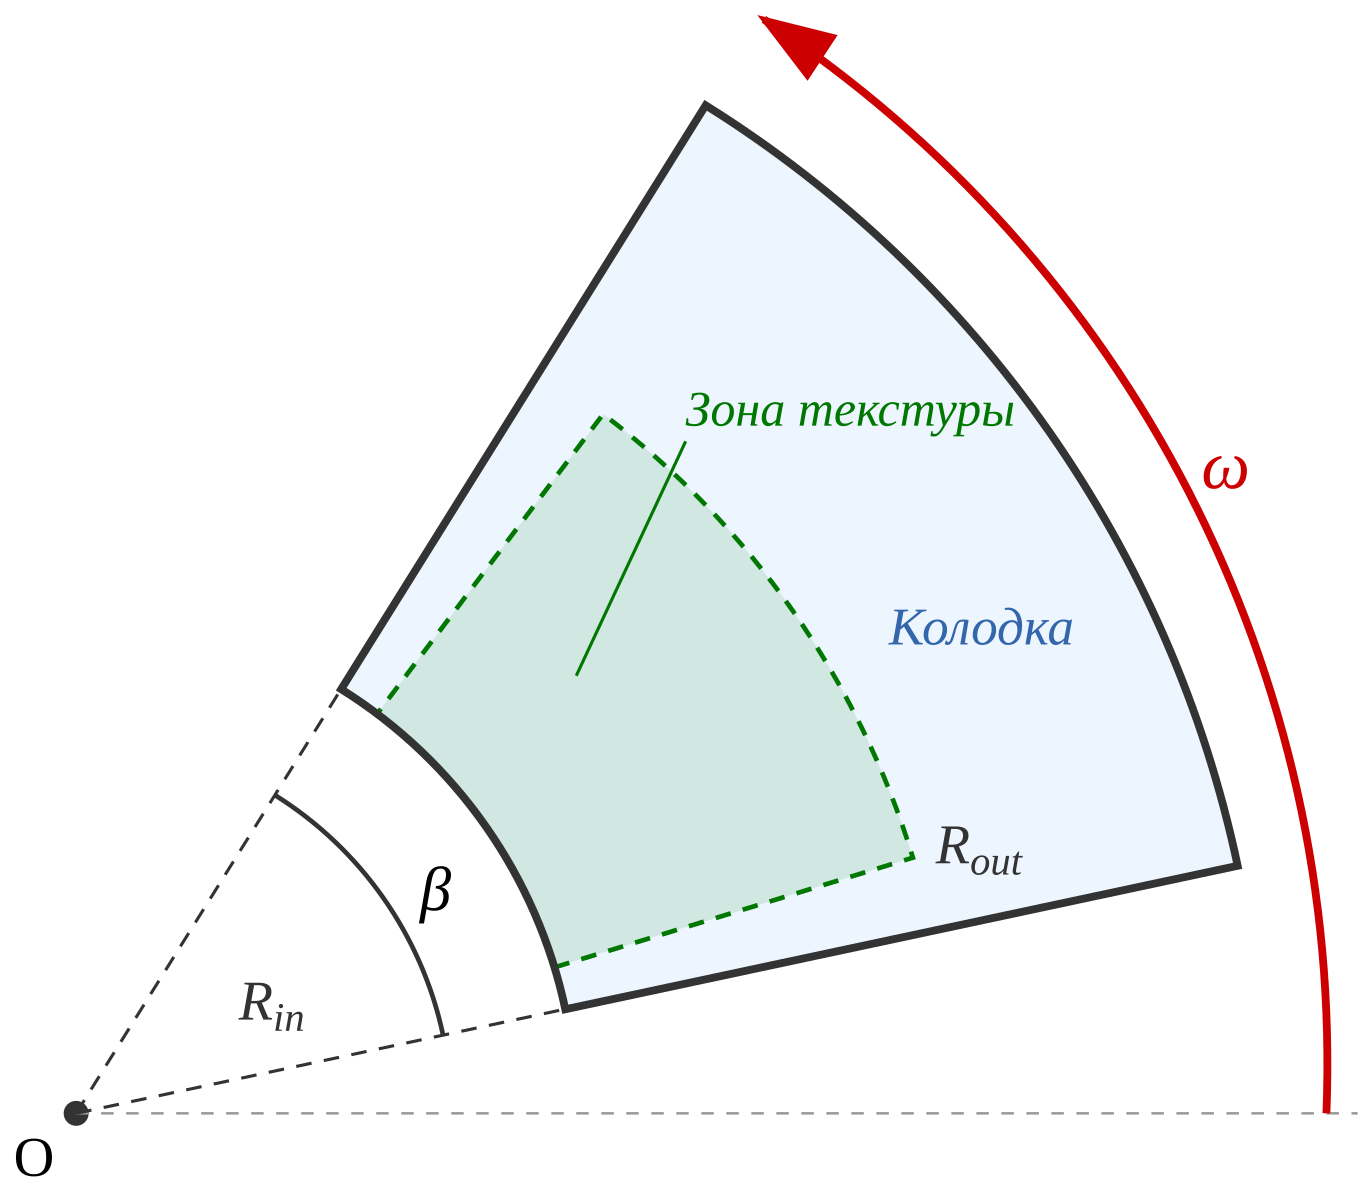
\includegraphics[width=\textwidth,height=0.9\textheight,keepaspectratio]{figures/ch07/fig_7_1.png}
\caption{Расчётная схема сектора упорного подшипника скольжения}
\label{fig:thrust_scheme}
\end{figure}

\FloatBarrier


\section{Расчётная схема и математическая модель}

Расчётная область представляет собой развёртку поверхности одного
сектора: $r \in [R_{\mathrm{in}},\, R_{\mathrm{out}}]$,
$\theta \in [0,\, \beta]$.

Угловая скорость вращения диска определяется частотой вращения:
\begin{equation}
  \omega = \frac{2\pi n}{60}.
  \label{eq:thrust_omega}
\end{equation}
Скорость скольжения на радиусе~$r$:
\begin{equation}
  U(r) = \omega \cdot r.
  \label{eq:thrust_U}
\end{equation}

Толщина смазочного зазора между колодкой и диском определяется
линейным законом клина:
\begin{equation}
  h(r, \theta) = h_{\mathrm{out}}
    + (h_{\mathrm{in}} - h_{\mathrm{out}})
    \left(1 - \frac{\theta}{\beta}\right)
  = h_{\mathrm{out}}
    \left[1 + (K - 1)\left(1 - \frac{\theta}{\beta}\right)\right],
  \label{eq:thrust_h}
\end{equation}
где $K = h_{\mathrm{in}} / h_{\mathrm{out}}$~-- параметр клина
($K > 1$). При $\theta = 0$ (входная кромка) зазор максимален
$h = h_{\mathrm{in}} = K \cdot h_{\mathrm{out}}$; при
$\theta = \beta$ (выходная кромка) зазор минимален
$h = h_{\mathrm{out}}$.

Распределение давления в смазочном слое описывается уравнением
Рейнольдса в цилиндрических координатах:
\begin{equation}
  \frac{\partial}{\partial r}
    \left[r\, h^3\, \frac{\partial p}{\partial r}\right]
  + \frac{\partial}{\partial \theta}
    \left[\frac{h^3}{r}\, \frac{\partial p}{\partial \theta}\right]
  = 6\mu\omega\, r\, \frac{\partial h}{\partial \theta}.
  \label{eq:thrust_reynolds}
\end{equation}

Граничные условия:
\begin{equation}
\left\{\;
\begin{aligned}
  p &= 0 \quad \text{при } \theta = 0
    \quad \text{(входная кромка)}, \\
  p &= 0 \quad \text{при } \theta = \beta
    \quad \text{(выходная кромка)}, \\
  p &= 0 \quad \text{при } r = R_{\mathrm{in}},\;
    r = R_{\mathrm{out}}.
\end{aligned}
\right.
  \label{eq:thrust_bc}
\end{equation}
Условие кавитации: $p \geq 0$.

Условия $p = 0$ на радиальных кромках представляют собой упрощение
модели, принятое для сравнительного анализа гладкого
и текстурированного вариантов на одной и той же расчётной области.

Интегральные характеристики подшипника вычисляются следующим
образом. Несущая сила:
\begin{equation}
  W = N_{\mathrm{pads}} \iint p\, r\, \mathrm{d}r\, \mathrm{d}\theta.
  \label{eq:thrust_W}
\end{equation}
Момент трения (упрощённая оценка; напорная составляющая
не учитывается):
\begin{equation}
  M_f = N_{\mathrm{pads}} \iint
    \frac{\mu\, \omega\, r}{h}\, r^2\,
    \mathrm{d}r\, \mathrm{d}\theta.
  \label{eq:thrust_Mf}
\end{equation}
Средний радиус:
\begin{equation}
  R_m = \frac{2}{3}\,
    \frac{R_{\mathrm{out}}^3 - R_{\mathrm{in}}^3}
         {R_{\mathrm{out}}^2 - R_{\mathrm{in}}^2}.
  \label{eq:thrust_Rm}
\end{equation}
Коэффициент трения:
\begin{equation}
  f_T = \frac{M_f}{W \cdot R_m}.
  \label{eq:thrust_fT}
\end{equation}
Расход смазочного материала:
\begin{equation}
  Q = N_{\mathrm{pads}} \int
    \left(-\frac{h^3}{12\mu}\,
    \frac{\partial p}{\partial r}\right)
    r\, \mathrm{d}\theta
    \bigg|_{r = R_{\mathrm{out}}}.
  \label{eq:thrust_Q}
\end{equation}
Максимальное давление в секторе:
$p_{\max} = \max\limits_{r,\theta} p(r, \theta)$.


\section{Конфигурации детерминированных микроструктур}

Аналогично главам~5 и~6, в качестве элементов рельефа используются
эллипсоидальные лунки~\eqref{eq:profile_ellipsoidal}
с шахматной раскладкой~\eqref{eq:layout_staggered}.
В координатах $(r, \theta)$ добавка от лунки записывается
в виде:
\begin{equation}
  \Delta h = H_p \cdot h_{\mathrm{out}}
    \left(1 - \frac{\Delta r^2}{a_r^2}
    - \frac{\Delta\theta^2}{a_\theta^2}\right)
  \quad \text{при}\quad
    \frac{\Delta r^2}{a_r^2}
    + \frac{\Delta\theta^2}{a_\theta^2} \leq 1,
  \label{eq:thrust_dimple}
\end{equation}
где $a_r$, $a_\theta$~-- полуоси эллипса в направлениях~$r$
и~$\theta$, $H_p$~-- безразмерная глубина лунки, нормированная
на~$h_{\mathrm{out}}$.

Конфигурации T1 и~T2 нанесены в зоне
$\theta \in [0{,}1\beta;\; 0{,}7\beta]$~-- входная и средняя
часть клина, где давление нарастает. Конфигурация~T3 нанесена
в зоне $\theta \in [0{,}3\beta;\; 0{,}9\beta]$~-- средняя
и выходная часть клина.

Ожидается, что текстурирование в зоне нарастания давления (T1,~T2)
эффективнее, чем в зоне спада (T3), поскольку лунки создают
дополнительные гидродинамические клинья именно там, где формируется
основная несущая способность.

Параметры рассматриваемых конфигураций приведены в
таблице~\ref{tab:thrust_texture}.

\begin{table}[!ht]
\centering
\caption{Параметры конфигураций текстуры упорного подшипника}
\label{tab:thrust_texture}
\begin{tabularx}{\textwidth}{|X|c|c|c|c|c|}
\hline
\multicolumn{1}{|c|}{\textbf{Конфигурация}}
  & $\boldsymbol{H_p}$
  & $\boldsymbol{A^*}$
  & $\boldsymbol{B^*}$
  & \textbf{Зона нанесения}
  & \textbf{Число лунок} \\
\hline
T1 & 0{,}20 & 0{,}060 & 0{,}025 & $0{,}1\beta$--$0{,}7\beta$ & $5 \times 8$ \\
\hline
T2 & 0{,}40 & 0{,}060 & 0{,}025 & $0{,}1\beta$--$0{,}7\beta$ & $5 \times 8$ \\
\hline
T3 & 0{,}20 & 0{,}060 & 0{,}025 & $0{,}3\beta$--$0{,}9\beta$ & $5 \times 8$ \\
\hline
\end{tabularx}
\end{table}

\FloatBarrier

Безразмерные полуоси определяются как
$A^* = a_r / (R_{\mathrm{out}} - R_{\mathrm{in}})$,
$B^* = a_\theta / \beta$.

Карта распределения зазора для конфигурации~T2 представлена
на рисунке~\ref{fig:thrust_texture_map}.

\begin{figure}[!ht]
\centering
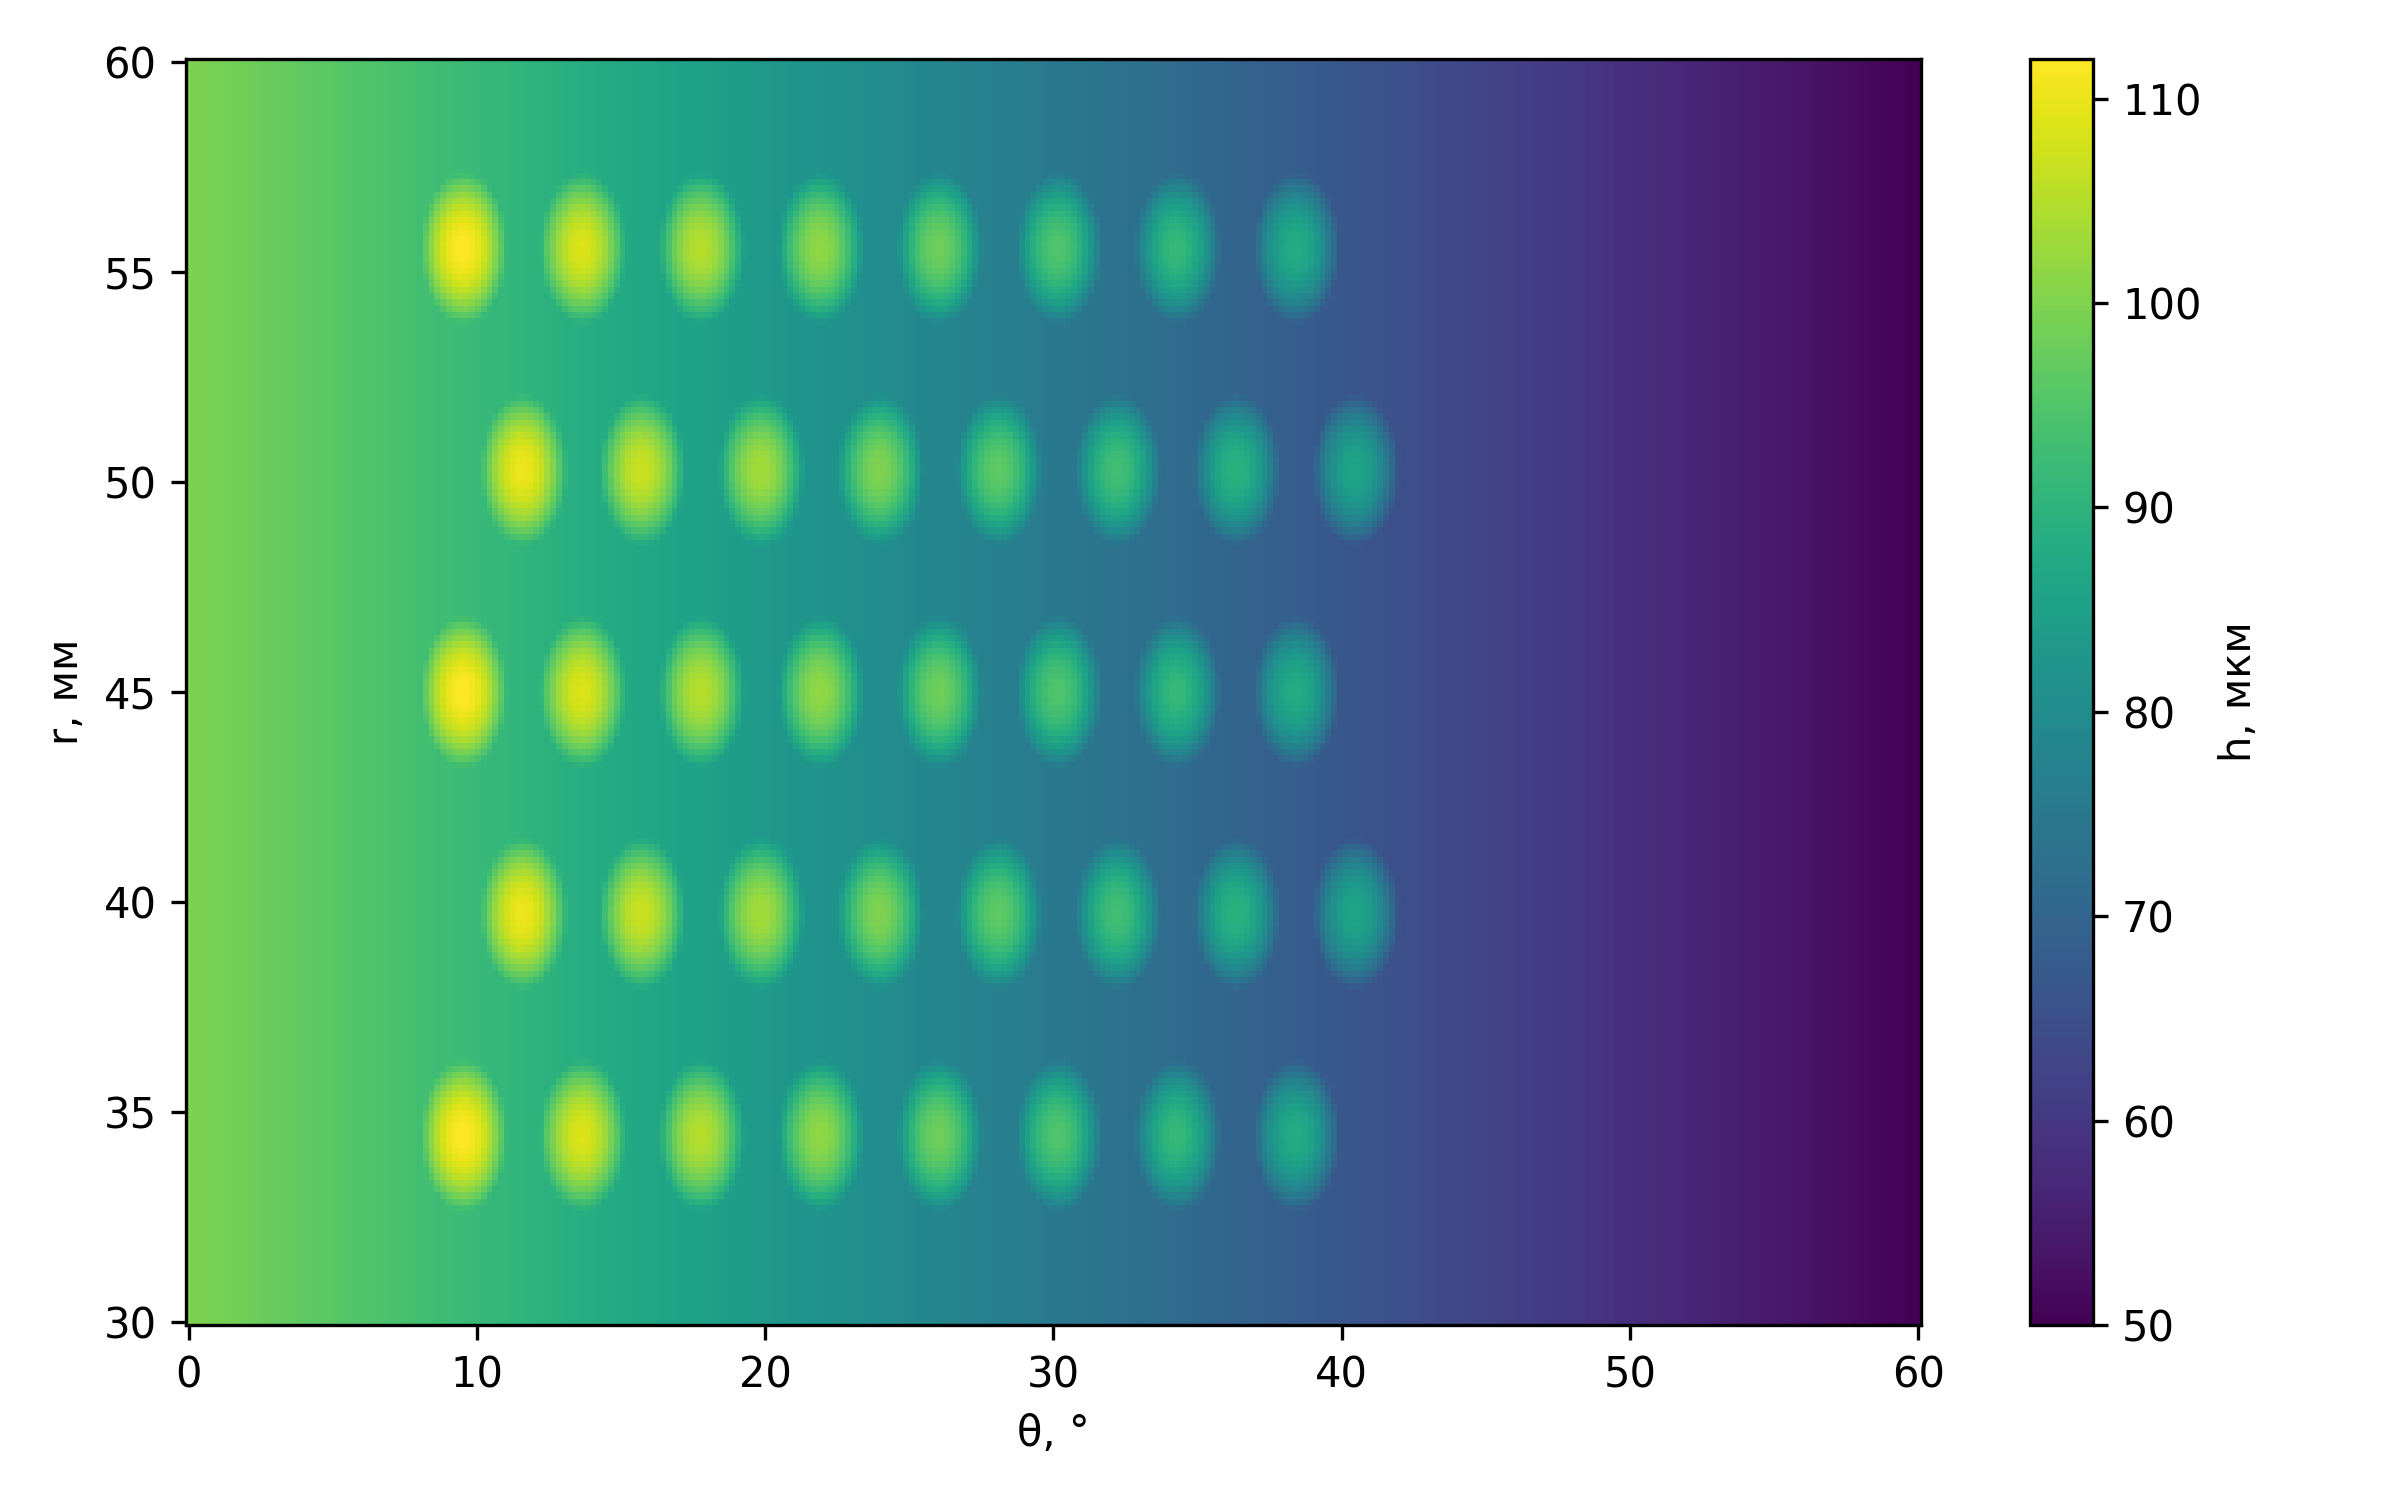
\includegraphics[width=\textwidth,height=0.9\textheight,keepaspectratio]{figures/ch07/fig_7_2.png}
\caption{Карта распределения зазора $h(r, \theta)$ в мкм
  для конфигурации~T2
  ($H_p = 0{,}40$, зона $0{,}1\beta$--$0{,}7\beta$) при $K = 2{,}0$.
  Светлые пятна~-- эллипсоидальные лунки.}
\label{fig:thrust_texture_map}
\end{figure}

\FloatBarrier


\section{Численная реализация расчёта}

Расчётная область дискретизируется равномерной сеткой
$200 \times 300$ узлов по~$r$ и~$\theta$. Уравнение
Рейнольдса~\eqref{eq:thrust_reynolds} аппроксимируется
центральными конечными разностями второго порядка точности.
Коэффициенты дивергентной формы вычисляются на полуузлах
$(i \pm 1/2,\; j \pm 1/2)$ с интерполяцией значений~$h$.

Полученная дискретная система решается итерационным
методом SOR (метод последовательной сверхрелаксации) с параметром
релаксации $\omega_{\mathrm{SOR}} = 1{,}5$. Критерий сходимости:
\begin{equation}
  \frac{\max |P_{\mathrm{new}} - P_{\mathrm{old}}|}
       {\max |P| + 10^{-10}} < 10^{-5}.
  \label{eq:thrust_convergence}
\end{equation}
Кавитация учитывается обнулением отрицательных давлений
на каждой итерации. Сходимость достигается за 2500--8000 итераций
в зависимости от~$K$ и конфигурации текстуры.


\section{Результаты при номинальном параметре клина}

При $K_{\mathrm{nom}} = 2{,}0$ проведён расчёт гладкого
подшипника и конфигураций T1, T2, T3. Результаты приведены
в таблице~\ref{tab:thrust_results}.

\begin{table}[!ht]
\centering
\caption{Характеристики упорного подшипника при $K_{\mathrm{nom}} = 2{,}0$}
\label{tab:thrust_results}
\begin{tabularx}{\textwidth}{|X|c|c|c|c|c|}
\hline
\multicolumn{1}{|c|}{\textbf{Вариант}}
  & $\boldsymbol{W}$, \textbf{кН}
  & $\boldsymbol{M_f}$, \textbf{Н$\cdot$м}
  & $\boldsymbol{f_T}$
  & $\boldsymbol{Q}$, \textbf{мл/с}
  & $\boldsymbol{p_{\max}}$, \textbf{МПа} \\
\hline
Гладкий & 1{,}82 & 1{,}6624 & 0{,}01953 & 26{,}595 & 0{,}510 \\
\hline
T1      & 1{,}84 & 1{,}6458 & 0{,}01912 & 27{,}007 & 0{,}536 \\
\hline
T2      & 1{,}85 & 1{,}6315 & 0{,}01889 & 27{,}324 & 0{,}552 \\
\hline
T3      & 1{,}79 & 1{,}6407 & 0{,}01963 & 26{,}406 & 0{,}523 \\
\hline
\end{tabularx}
\end{table}

\FloatBarrier

В рассматриваемой постановке минимальный зазор определяется
выходной кромкой колодки:
$h_{\min} = h_{\mathrm{out}} = 50$~мкм для всех вариантов
при фиксированной геометрии колодки, поэтому показатель
$G_{h_{\min}} = 1$ для всех конфигураций.

Нормированные показатели эффективности вычисляются аналогично
главам~5 и~6:
\begin{equation}
\begin{split}
  &G_W = \frac{W_{\mathrm{tex}}}{W_{\mathrm{smooth}}}, \quad
  G_{M_f} = \frac{M_{f,\mathrm{smooth}}}{M_{f,\mathrm{tex}}}, \\
  &G_{f_T} = \frac{f_{T,\mathrm{smooth}}}{f_{T,\mathrm{tex}}}, \quad
  G_Q = \frac{Q_{\mathrm{smooth}}}{Q_{\mathrm{tex}}}, \quad
  G_{p_{\max}} = \frac{p_{\max,\mathrm{smooth}}}{p_{\max,\mathrm{tex}}}.
\end{split}
  \label{eq:thrust_gains}
\end{equation}
Значение~$G > 1$ желательно для~$G_W$, $G_{M_f}$, $G_{f_T}$
(рост несущей способности, снижение момента трения и коэффициента
трения); для~$G_Q$ и~$G_{p_{\max}}$ значение~$G > 1$ означает
снижение расхода и пикового давления. Результаты сведены
в таблицу~\ref{tab:thrust_gains}.

\begin{table}[!ht]
\centering
\caption{Нормированные показатели эффективности
  при $K_{\mathrm{nom}} = 2{,}0$}
\label{tab:thrust_gains}
\begin{tabularx}{\textwidth}{|X|c|c|c|c|c|}
\hline
\multicolumn{1}{|c|}{\textbf{Вариант}}
  & $\boldsymbol{G_W}$
  & $\boldsymbol{G_{M_f}}$
  & $\boldsymbol{G_{f_T}}$
  & $\boldsymbol{G_Q}$
  & $\boldsymbol{G_{p_{\max}}}$ \\
\hline
T1 & 1{,}0107 & 1{,}0101 & 1{,}0209 & 0{,}9847 & 0{,}9517 \\
\hline
T2 & 1{,}0145 & 1{,}0189 & 1{,}0337 & 0{,}9733 & 0{,}9228 \\
\hline
T3 & 0{,}9816 & 1{,}0132 & 0{,}9946 & 1{,}0071 & 0{,}9738 \\
\hline
\end{tabularx}
\end{table}

\FloatBarrier

Конфигурации T1 и~T2, расположенные во входной и средней части
клина, обеспечивают умеренный рост несущей способности:
$G_W = 1{,}0107$ и $1{,}0145$. Коэффициент трения снижается:
$G_{f_T} = 1{,}0209$ и $1{,}0337$ ($G_{f_T} > 1$ означает снижение
$f_T$). Прирост~$W$ сопровождается увеличением расхода~$Q$
и максимального давления~$p_{\max}$
($G_Q < 1$, $G_{p_{\max}} < 1$).

Конфигурация~T3, нанесённая в средней и выходной части клина,
снижает несущую способность ($G_W = 0{,}9816 < 1$) и не улучшает
коэффициент трения ($G_{f_T} = 0{,}9946 < 1$). Это подтверждает
гипотезу: текстура в зоне убывания давления неэффективна.

Таким образом, текстурирование во входной и средней зоне (T1,~T2)
улучшает несущую способность и трение, однако увеличивает утечки
и пиковое давление. Наилучший баланс демонстрирует
конфигурация~T2: $G_W = 1{,}0145$, $G_{f_T} = 1{,}0337$,
$G_{p_{\max}} = 0{,}9228$.

Нормированные показатели наглядно сопоставлены на
рисунке~\ref{fig:thrust_gains}.

\begin{figure}[!ht]
\centering
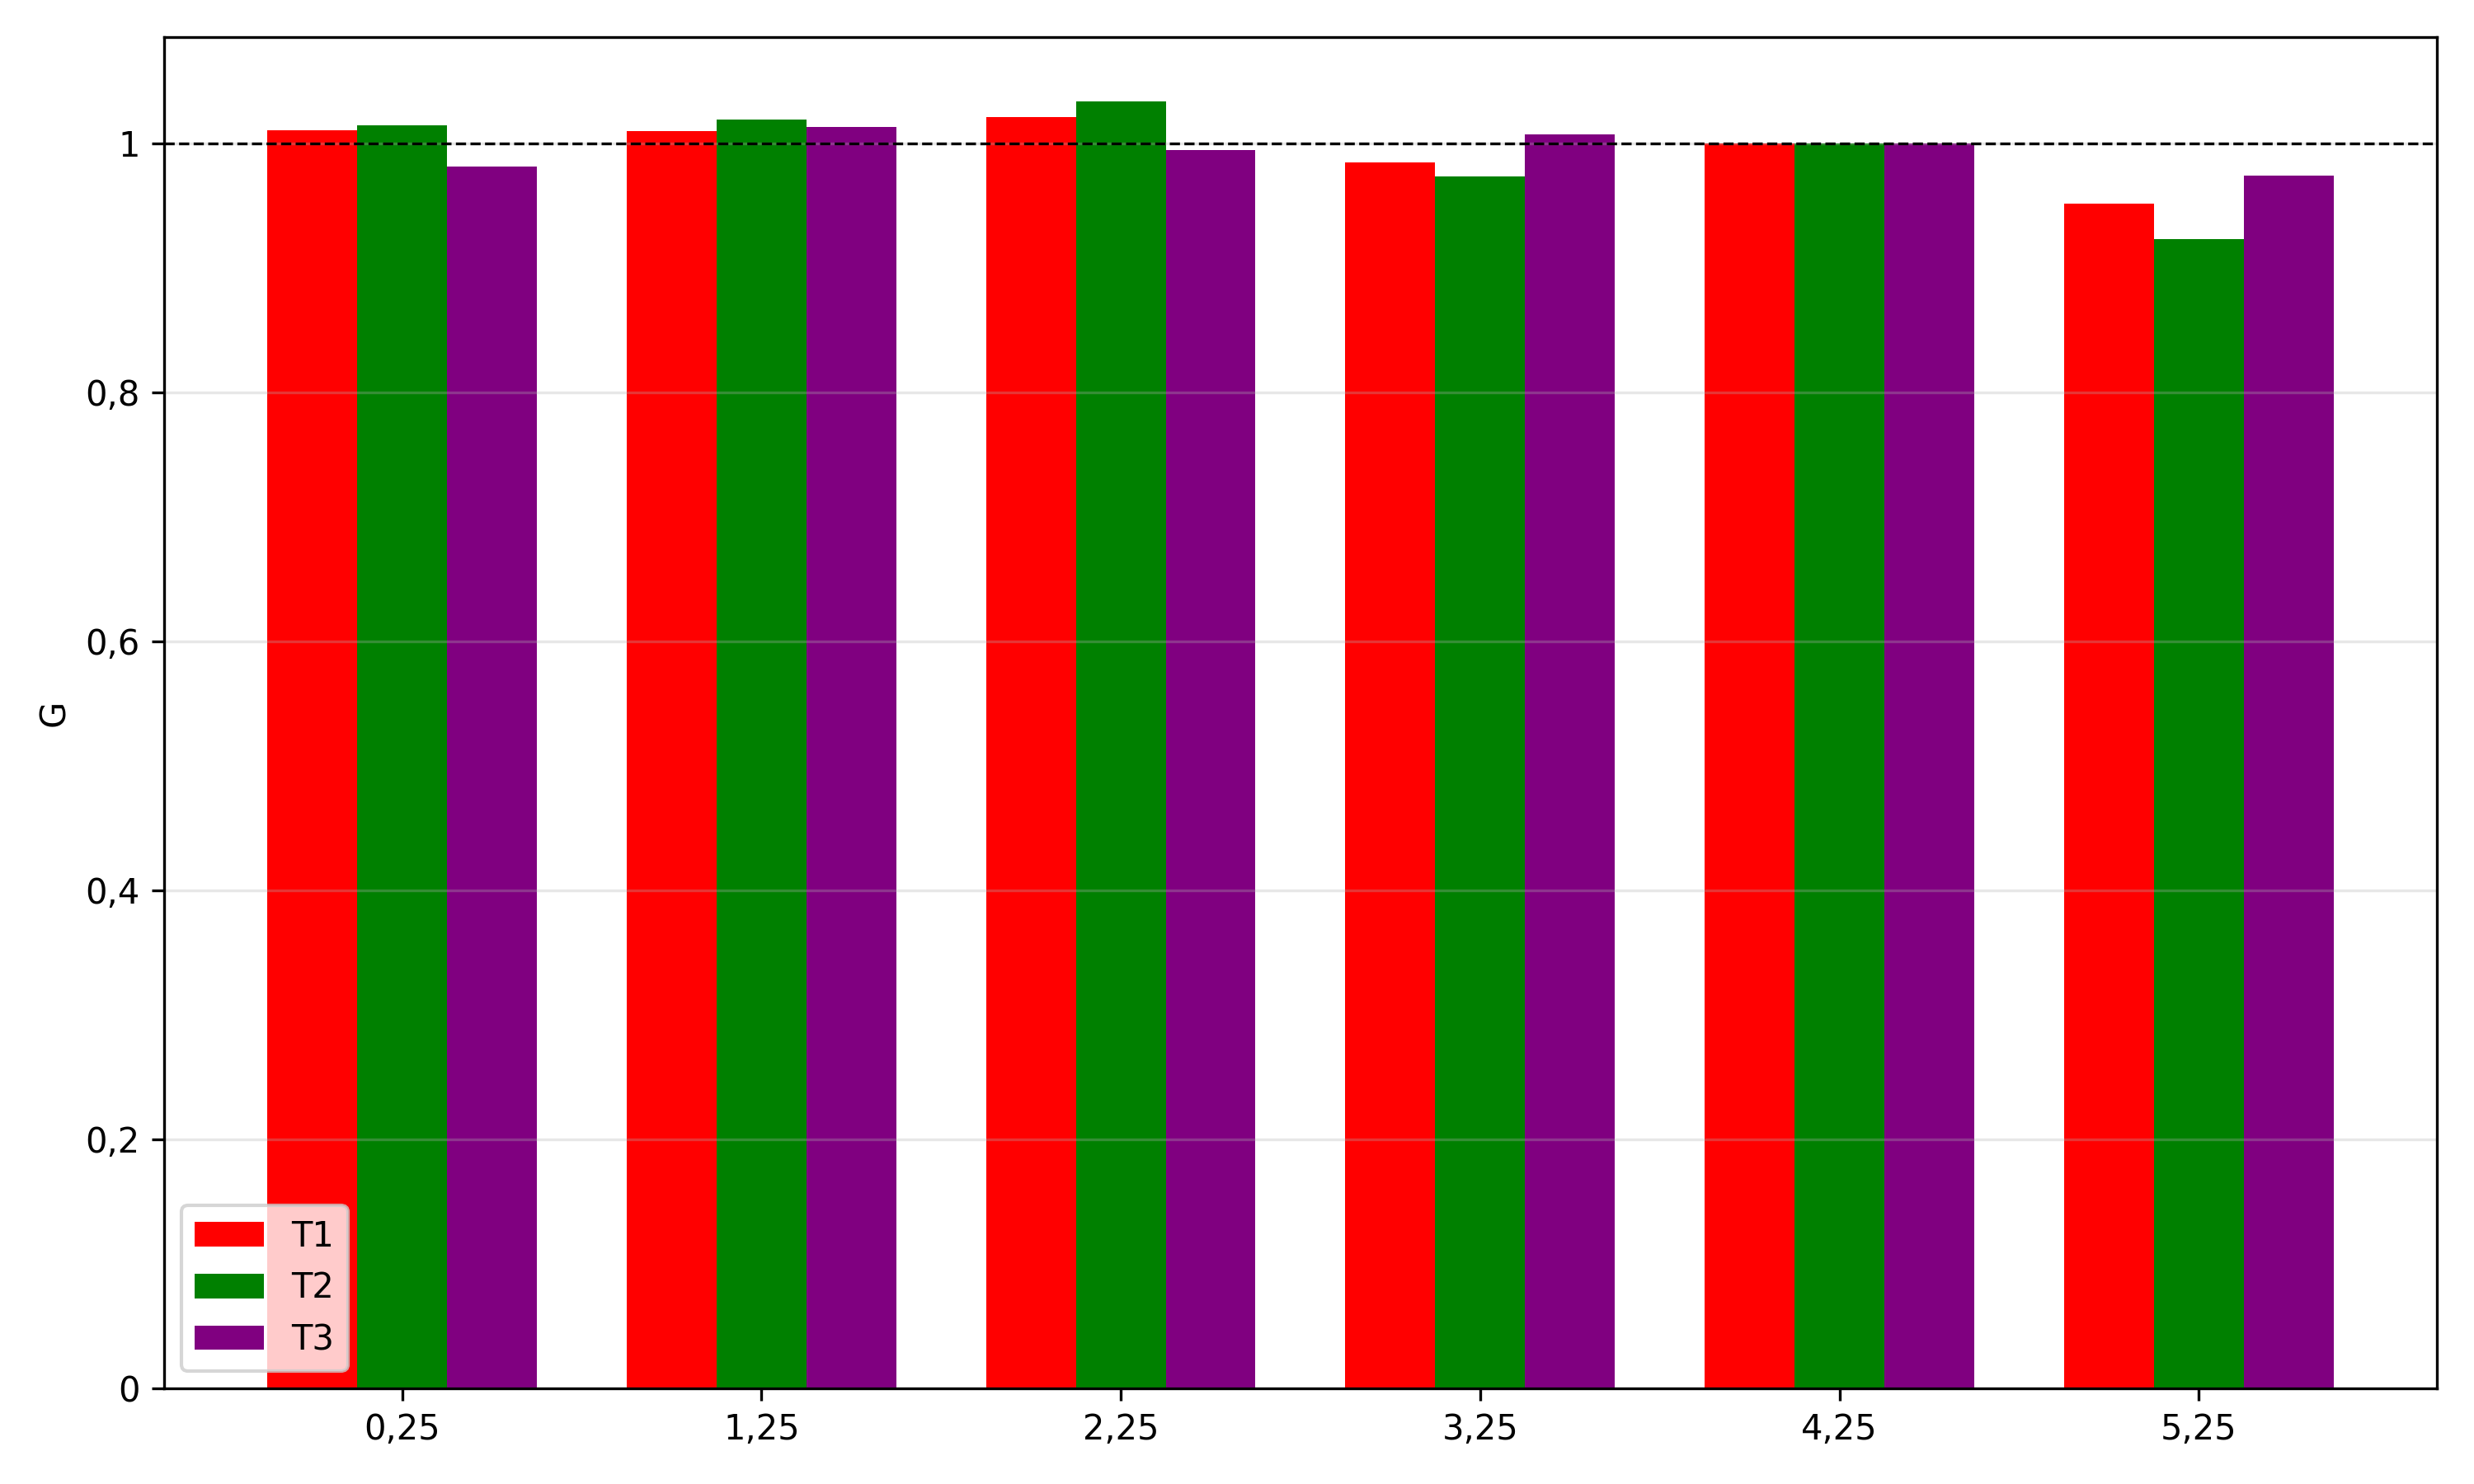
\includegraphics[width=\textwidth,height=0.9\textheight,keepaspectratio]{figures/ch07/fig_7_3.png}
\caption{Нормированные показатели эффективности $G_W$, $G_{M_f}$,
  $G_{f_T}$, $G_Q$, $G_{p_{\max}}$ для конфигураций T1, T2, T3
  при $K_{\mathrm{nom}} = 2{,}0$. Пунктирная горизонталь $G = 1$~--
  уровень гладкого подшипника.}
\label{fig:thrust_gains}
\end{figure}

\FloatBarrier


\section{Влияние параметра клина на рабочие характеристики}

Параметрический расчёт выполнен для
$K \in \{1{,}5;\; 2{,}0;\; 2{,}5;\; 3{,}0;\; 3{,}5;\; 4{,}0\}$.

\textit{Несущая сила.}
Несущая сила~$W$ имеет максимум при $K \approx 2{,}5$ для всех
вариантов (рисунок~\ref{fig:thrust_W_vs_K})~-- классическая
особенность клинового подшипника: при малых~$K$ клин слаб,
при больших~$K$ зазор~$h_{\mathrm{in}}$ слишком велик и давление
падает. Конфигурация~T2 превышает гладкий вариант по всему
диапазону~$K$. Конфигурация~T3 уступает гладкому при всех~$K$.

\begin{figure}[!ht]
\centering
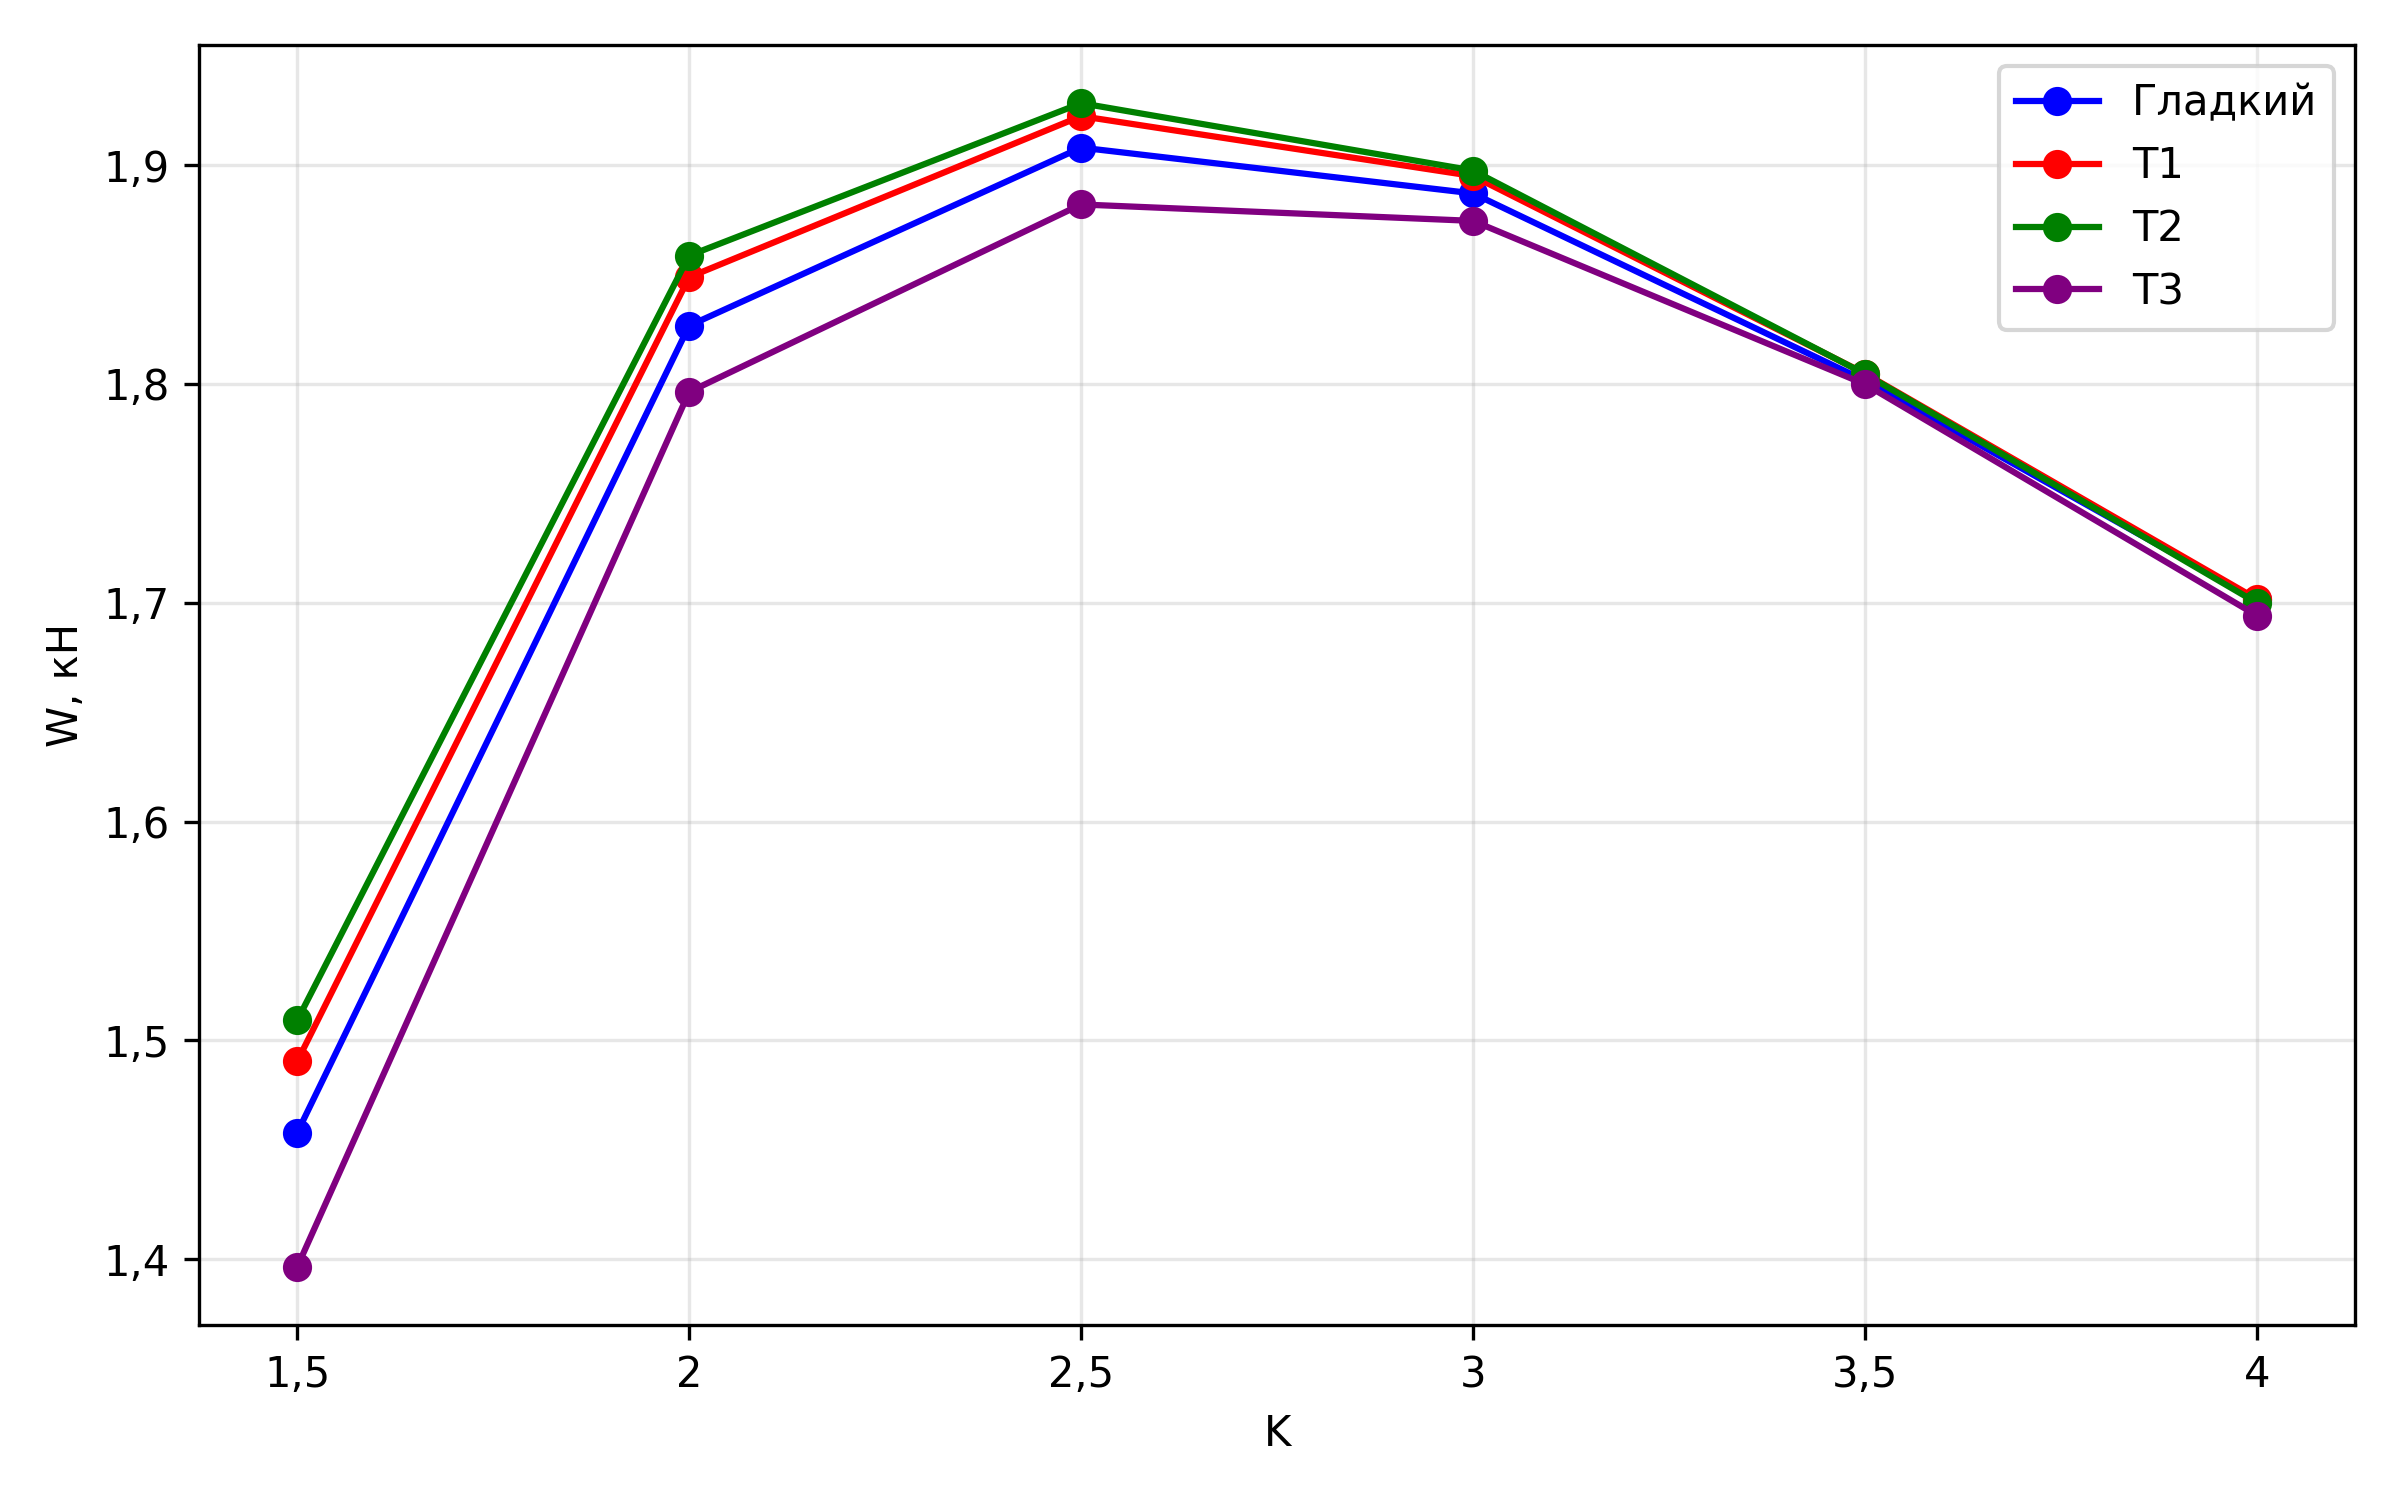
\includegraphics[width=\textwidth,height=0.9\textheight,keepaspectratio]{figures/ch07/fig_7_4.png}
\caption{Зависимость несущей силы $W$ от параметра клина $K$
  для гладкого подшипника и конфигураций T1, T2, T3.}
\label{fig:thrust_W_vs_K}
\end{figure}

\FloatBarrier

\textit{Коэффициент трения.}
Коэффициент трения~$f_T$ монотонно убывает с ростом~$K$
(рисунок~\ref{fig:thrust_fT_vs_K}). Конфигурация~T2 имеет
наименьший~$f_T$ при всех~$K$; конфигурация~T3 близка к гладкому
варианту или незначительно хуже.

\begin{figure}[!ht]
\centering
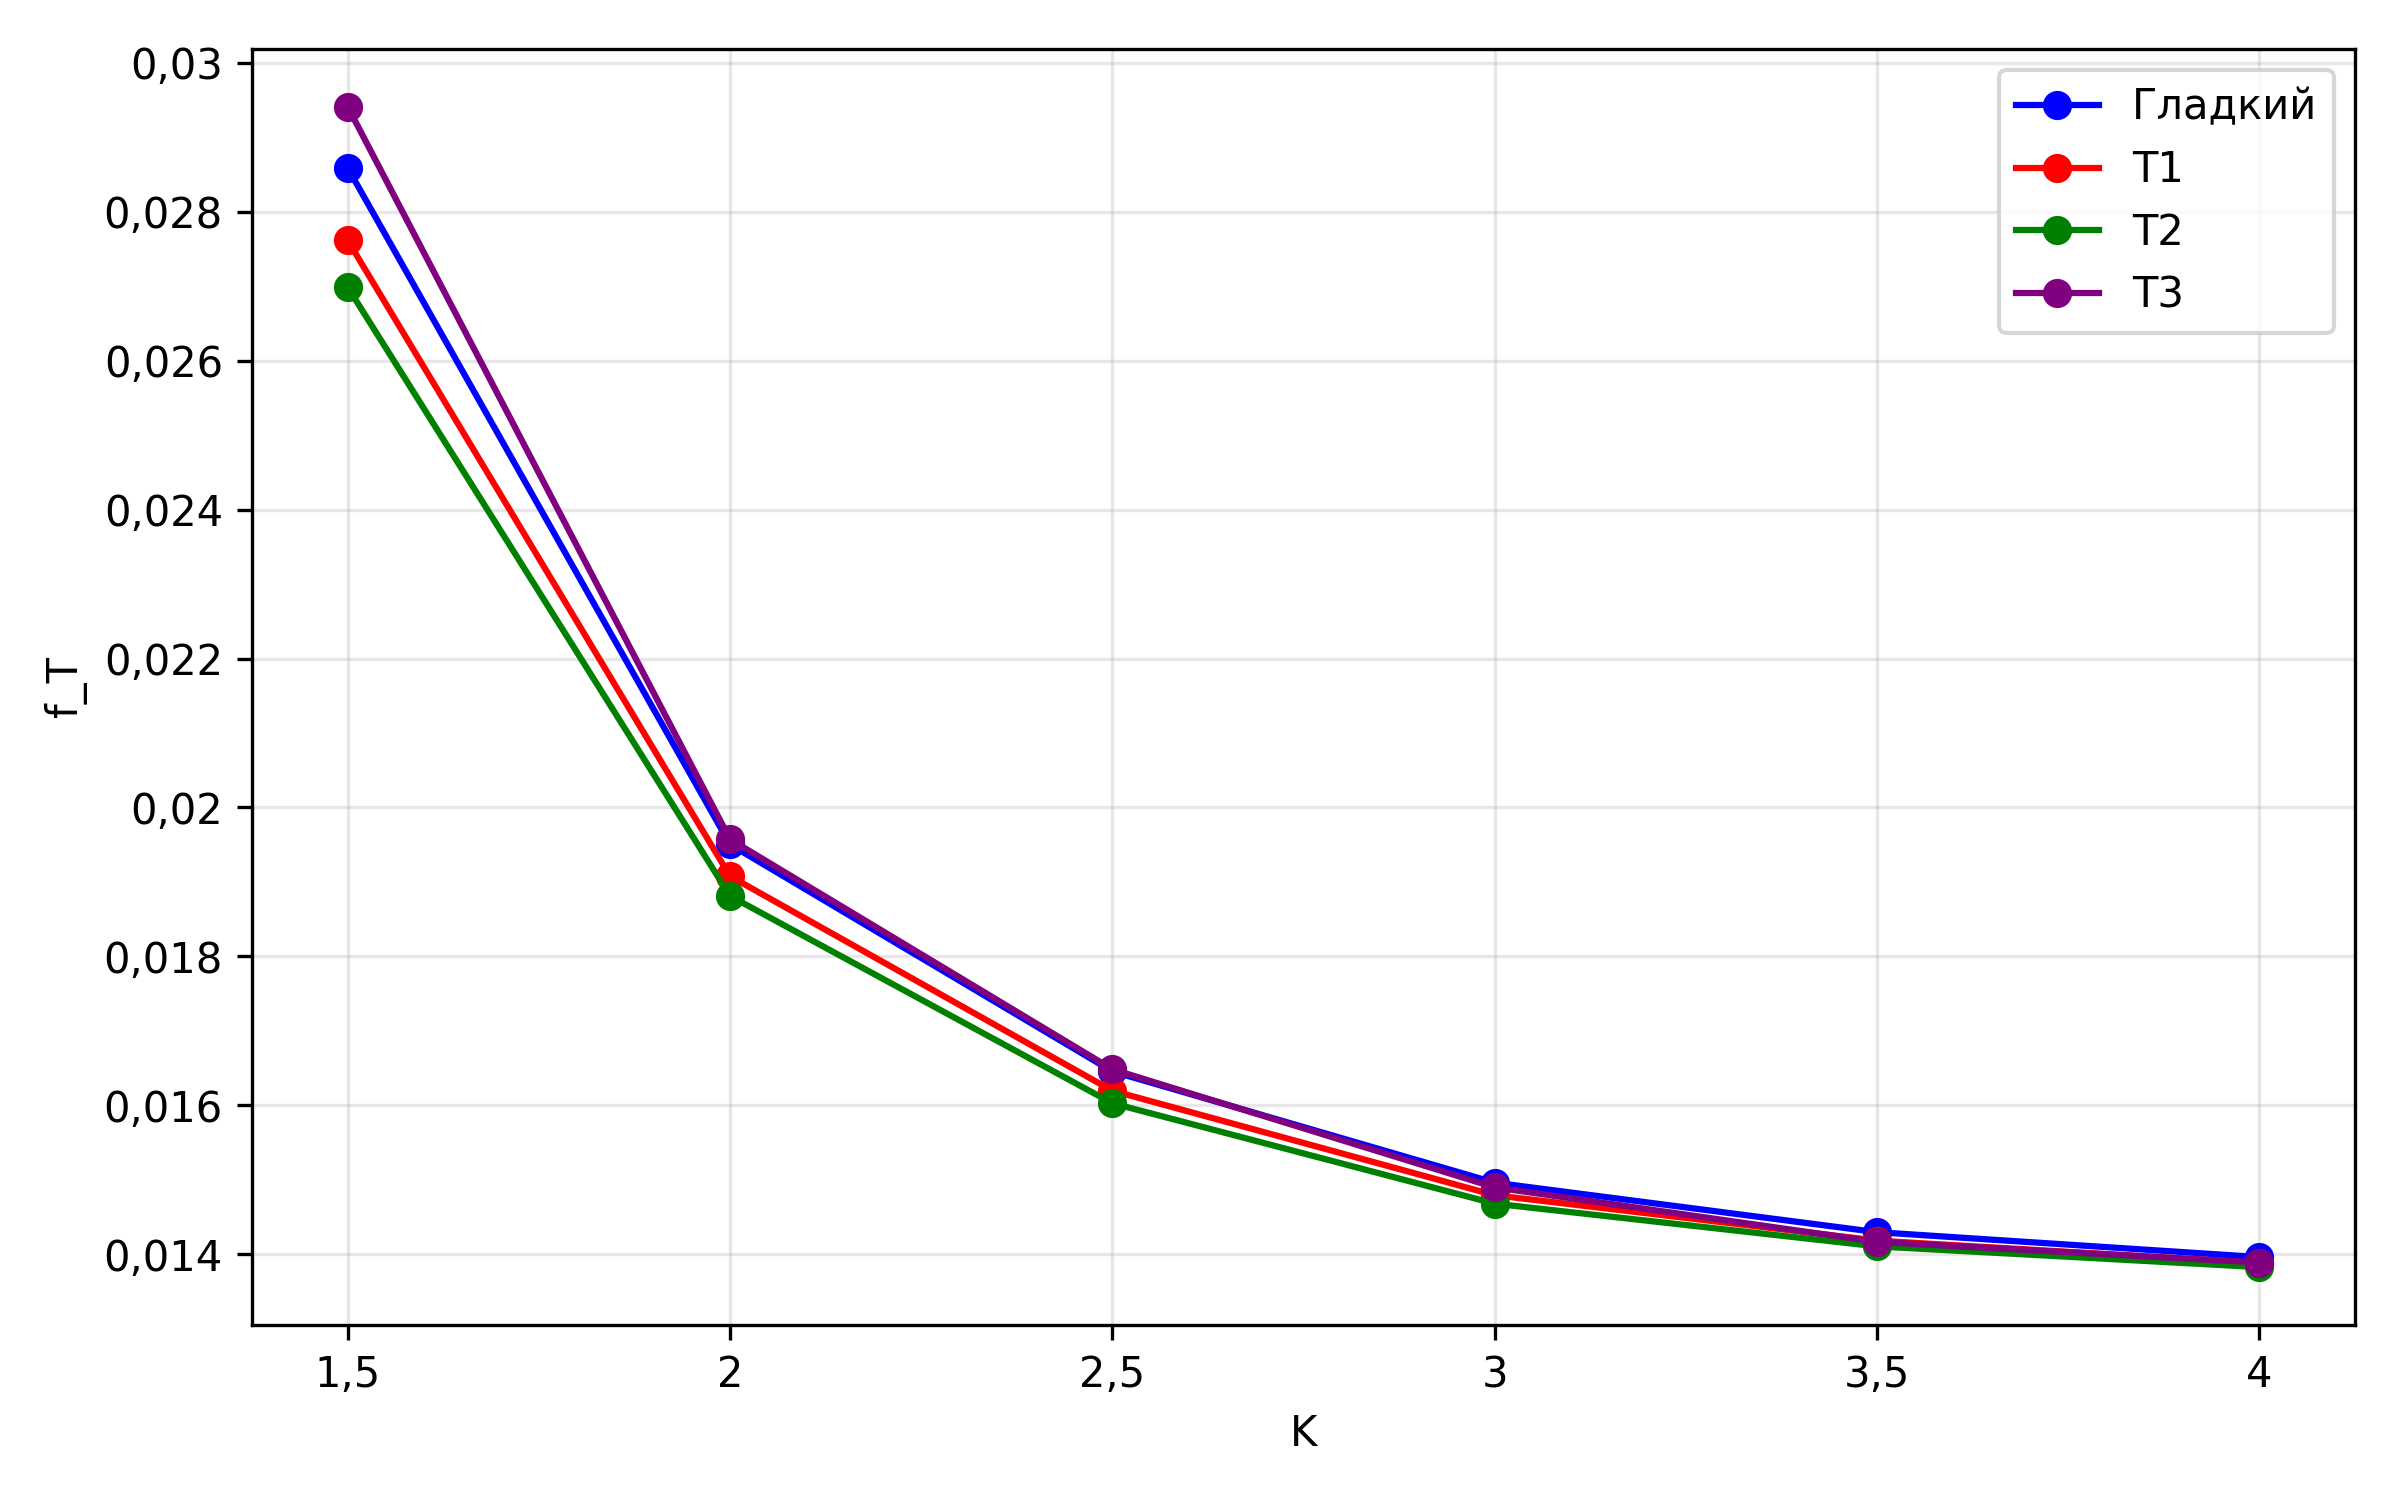
\includegraphics[width=\textwidth,height=0.9\textheight,keepaspectratio]{figures/ch07/fig_7_5.png}
\caption{Зависимость коэффициента трения $f_T$ от параметра
  клина $K$.}
\label{fig:thrust_fT_vs_K}
\end{figure}

\FloatBarrier

\textit{Расход смазочного материала.}
Расход~$Q$ монотонно растёт с~$K$
(рисунок~\ref{fig:thrust_Q_vs_K}). Различия между вариантами
невелики ($\leq 5\,\%$); конфигурация~T2 имеет несколько больший
расход вследствие увеличенного объёма лунок.

\begin{figure}[!ht]
\centering
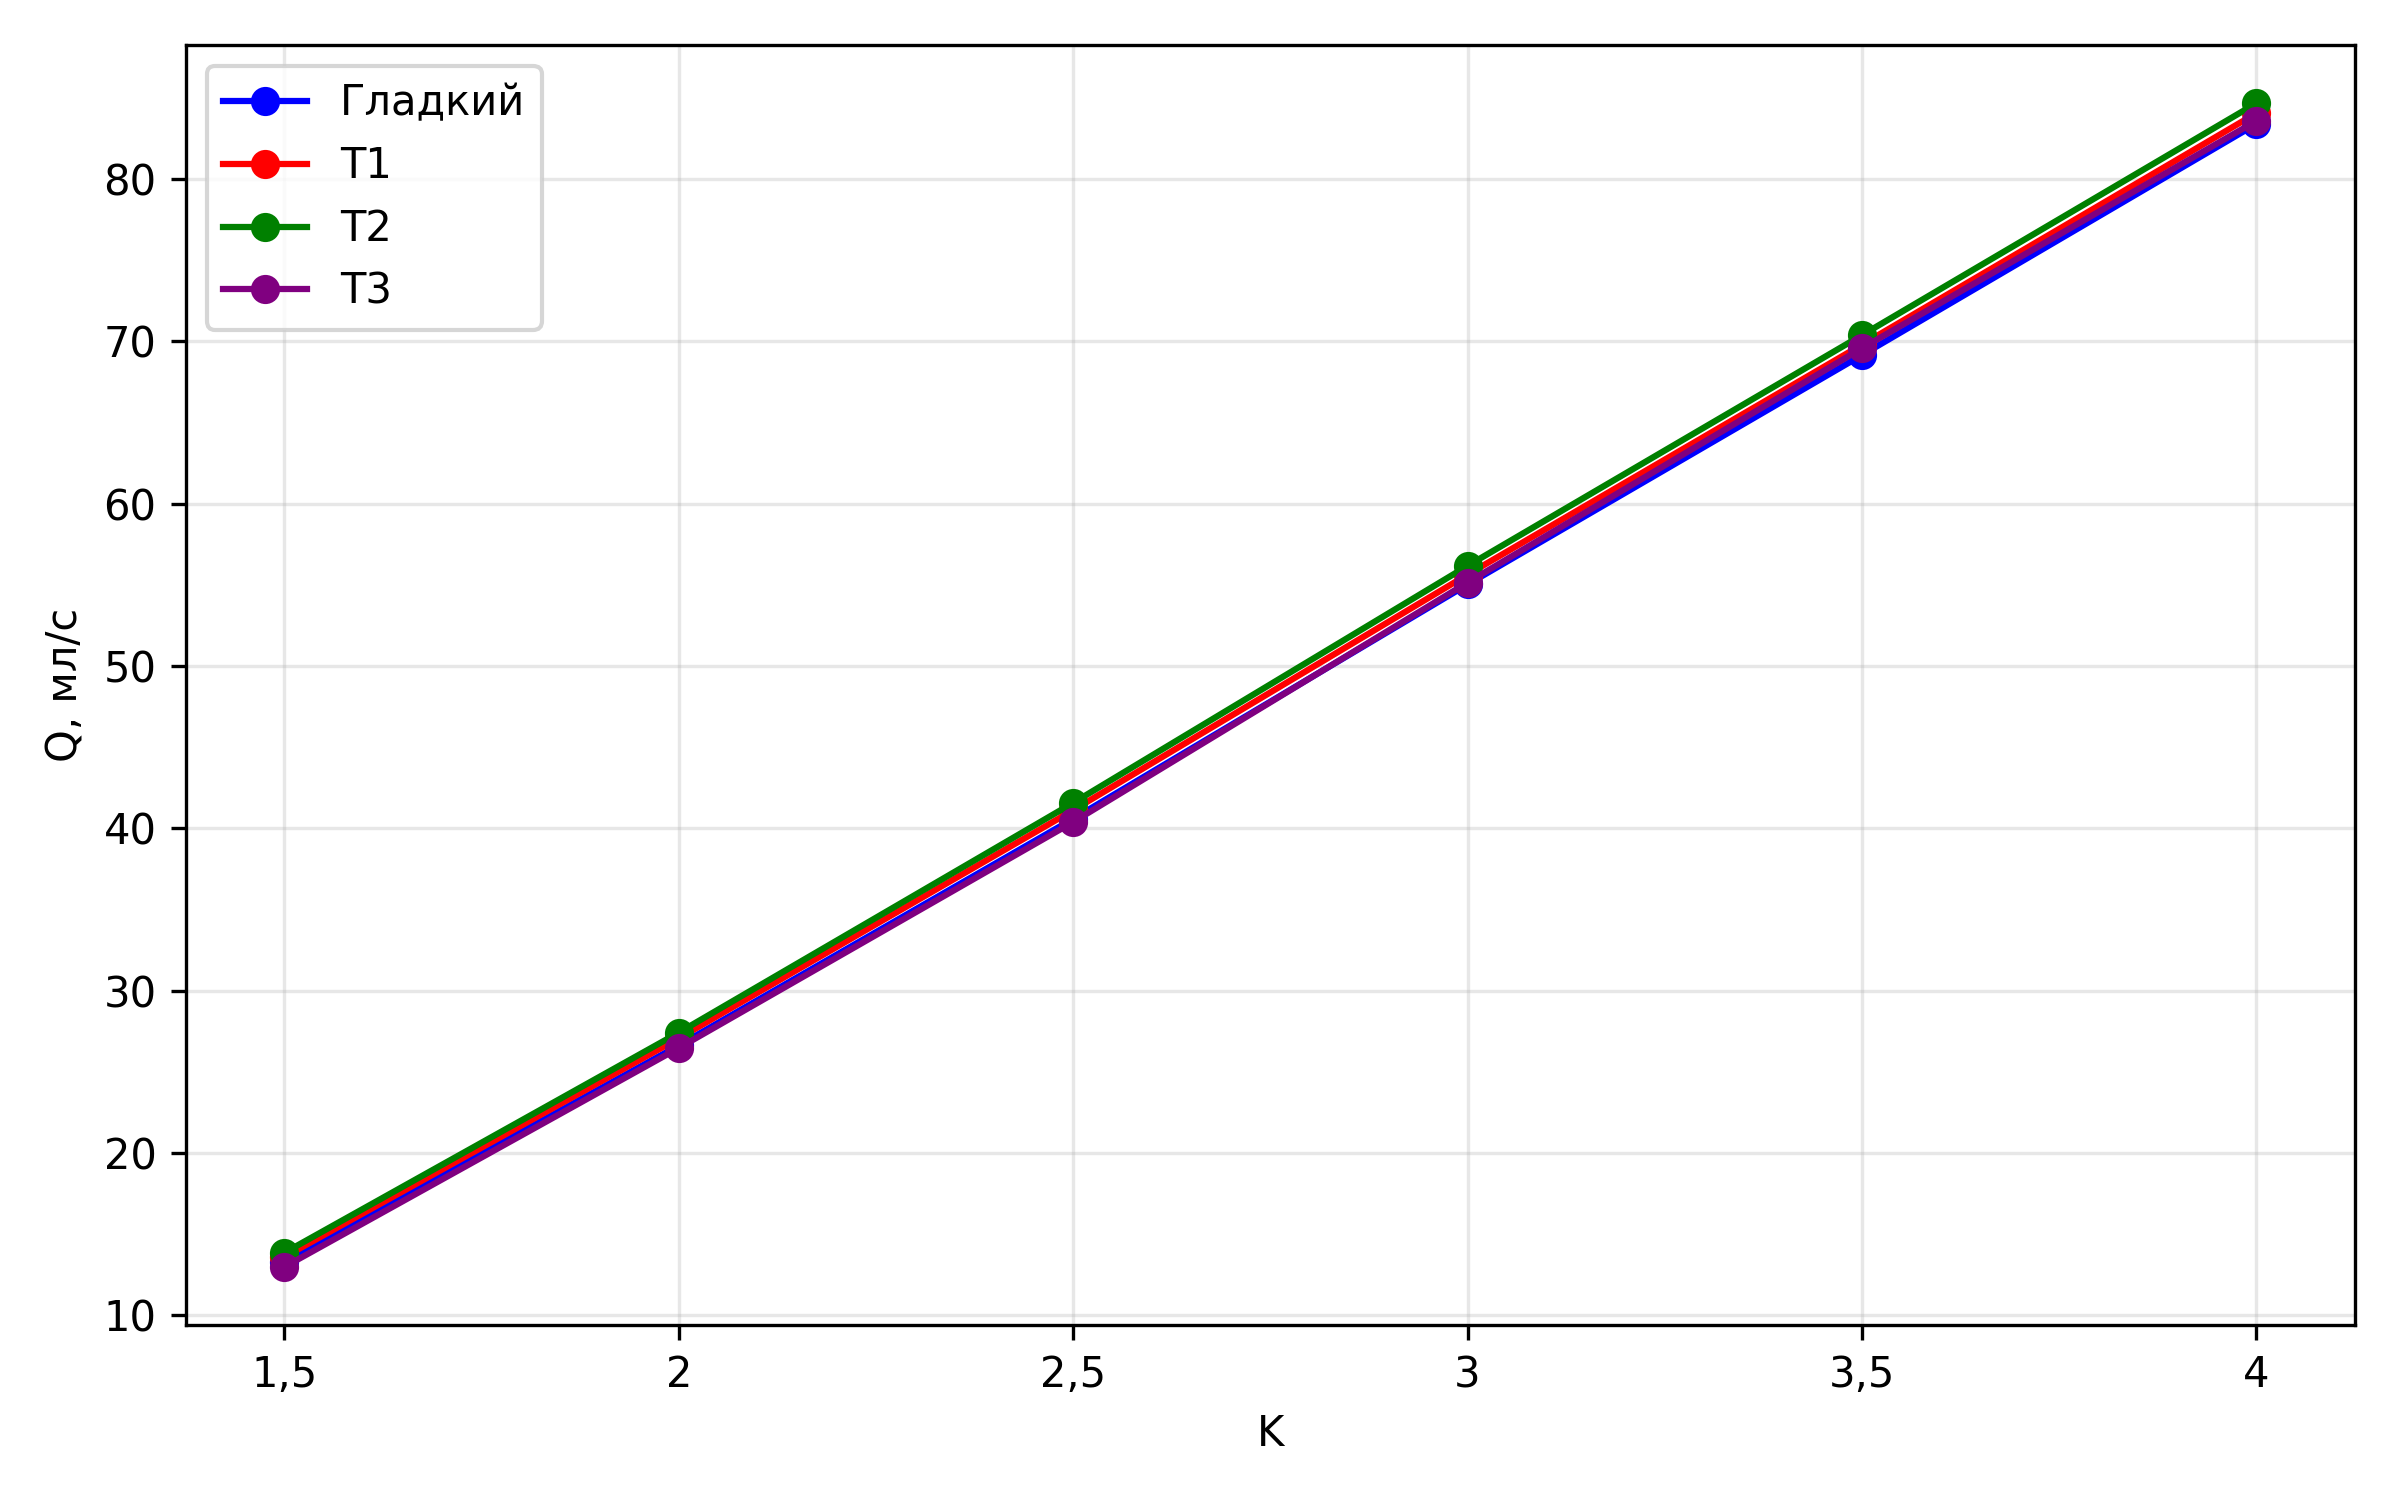
\includegraphics[width=\textwidth,height=0.9\textheight,keepaspectratio]{figures/ch07/fig_7_6.png}
\caption{Зависимость расхода смазки $Q$ от параметра клина $K$.}
\label{fig:thrust_Q_vs_K}
\end{figure}

\FloatBarrier

\textit{Максимальное давление.}
Максимальное давление~$p_{\max}$ растёт с~$K$ и достигает
насыщения при $K \approx 3$--$4$
(рисунок~\ref{fig:thrust_pmax_vs_K}). Конфигурации~T2 и~T1
демонстрируют более высокое~$p_{\max}$ по сравнению с гладким
вариантом; конфигурация~T3~-- ниже при малых~$K$ и выше
при больших~$K$.

\begin{figure}[!ht]
\centering
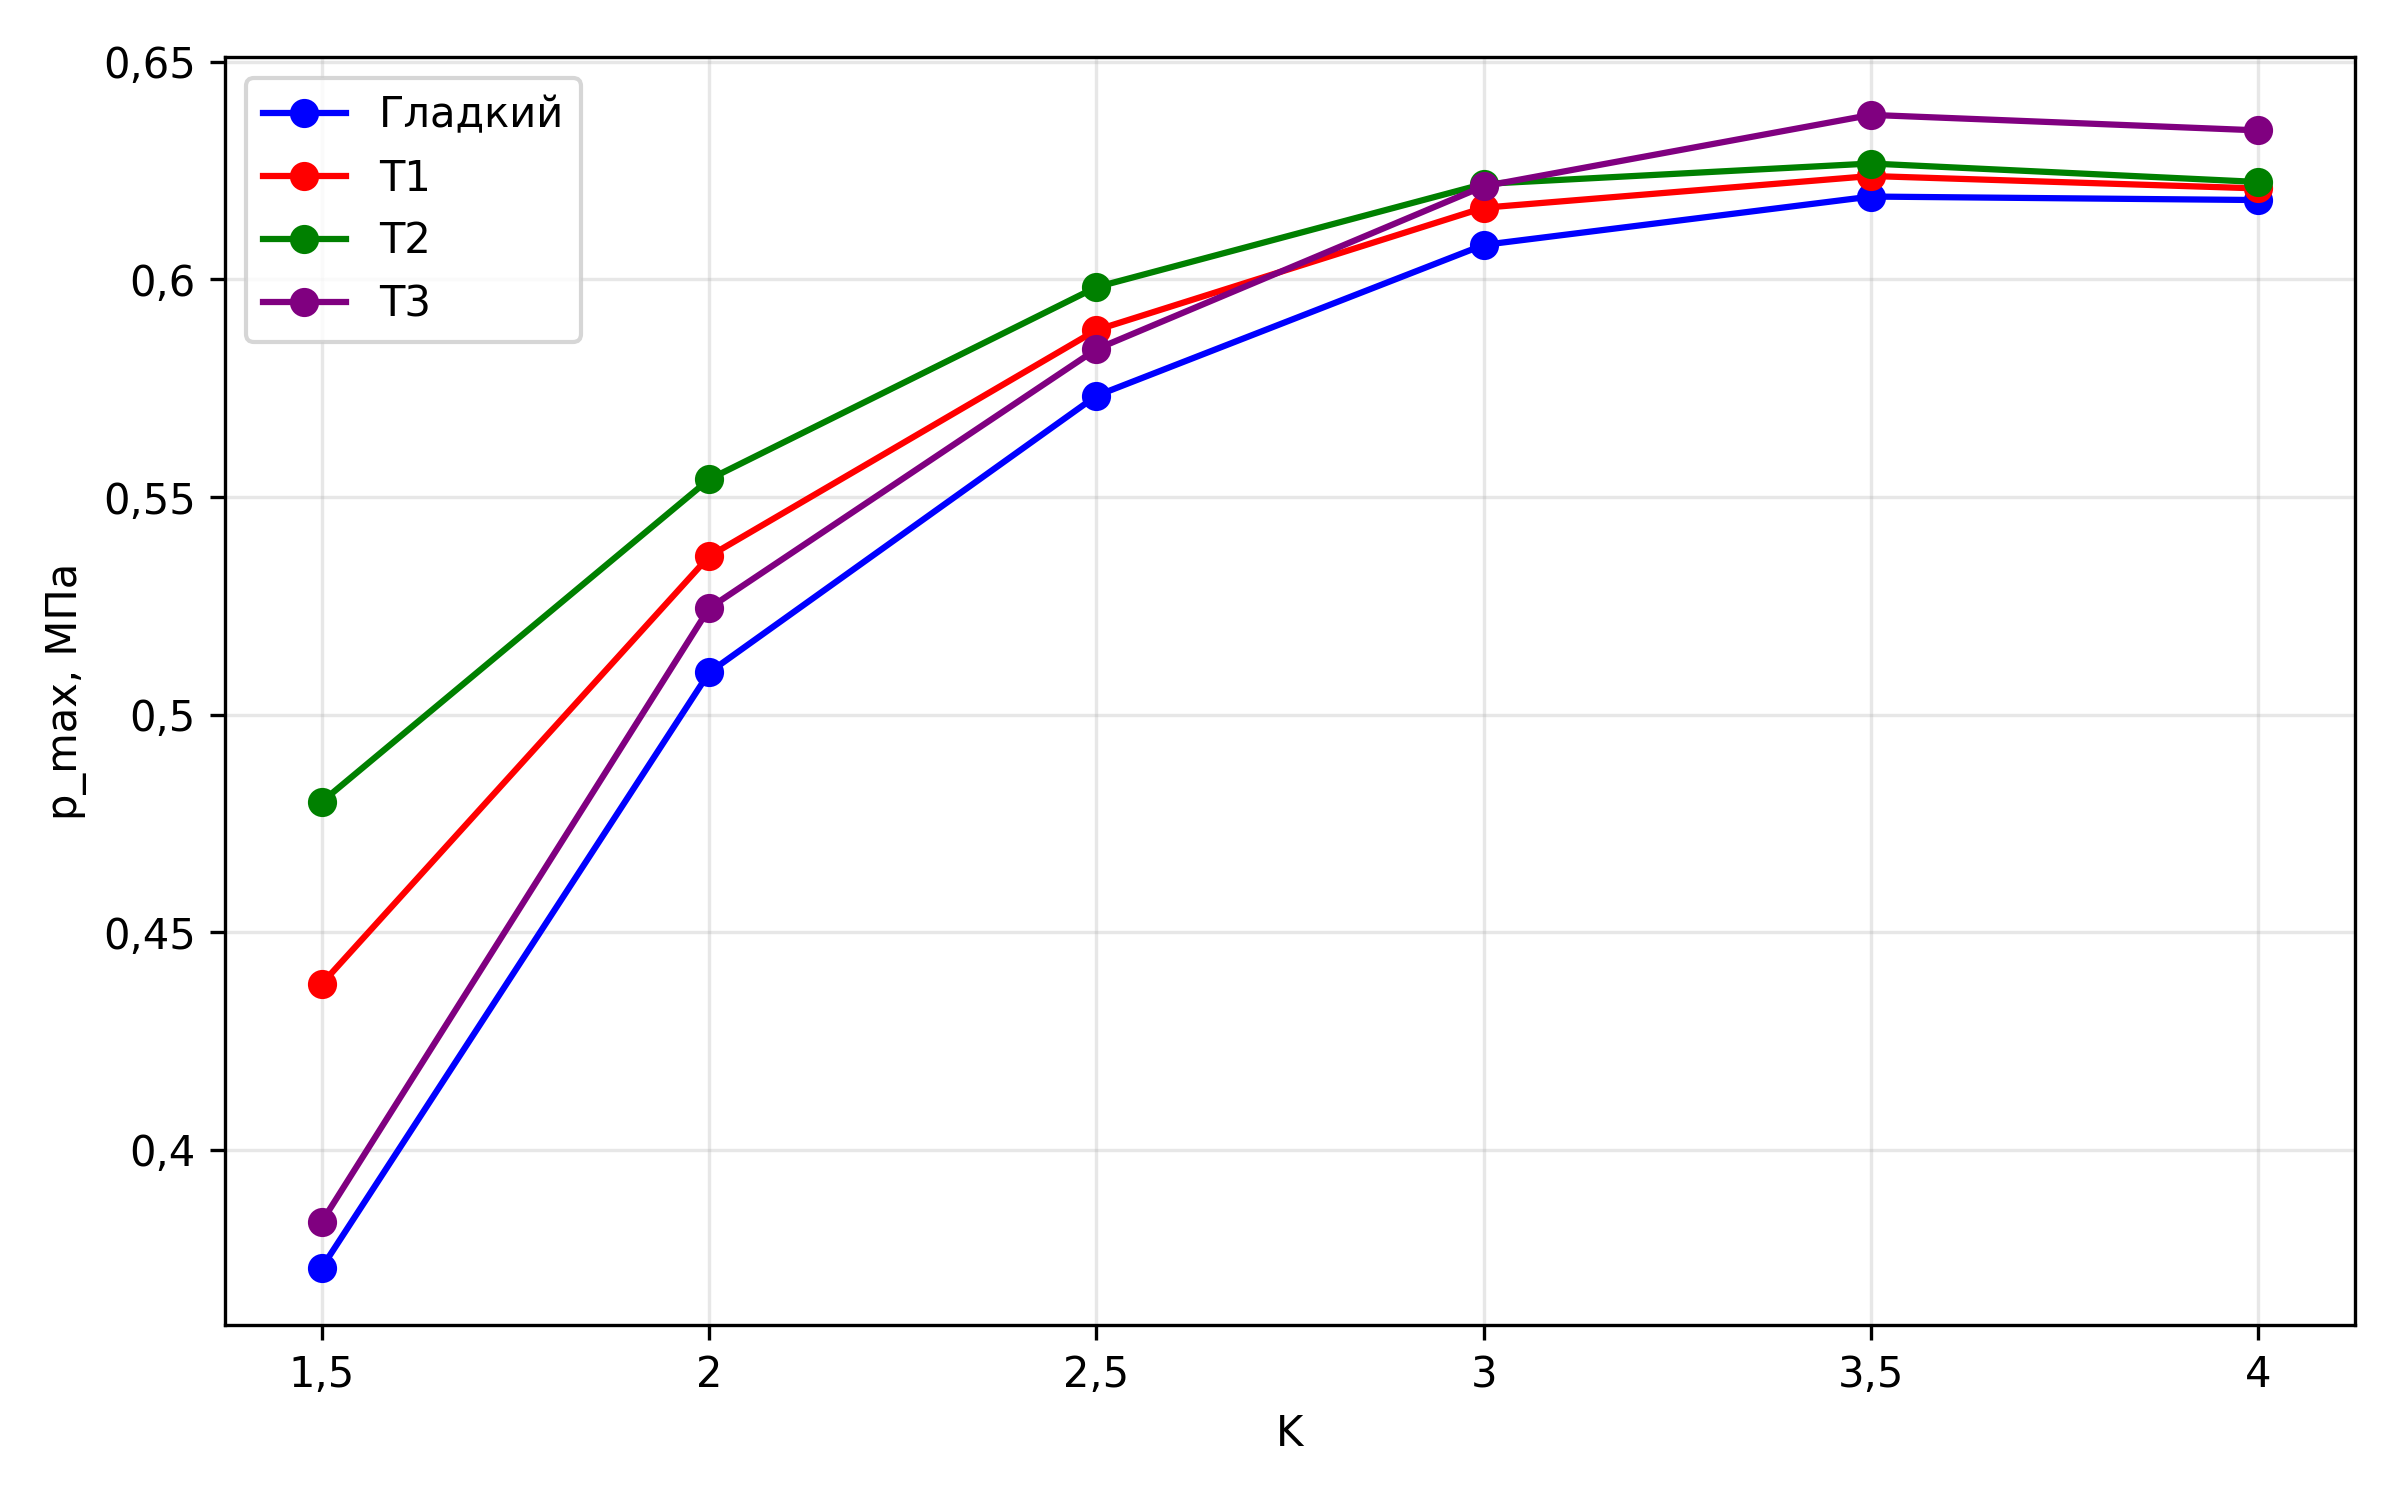
\includegraphics[width=\textwidth,height=0.9\textheight,keepaspectratio]{figures/ch07/fig_7_7.png}
\caption{Зависимость максимального давления $p_{\max}$ от параметра
  клина $K$.}
\label{fig:thrust_pmax_vs_K}
\end{figure}

\FloatBarrier

\textit{Минимальный зазор.}
В рассматриваемой постановке минимальный зазор определяется
выходной кромкой колодки:
$h_{\min} = h_{\mathrm{out}} = 50$~мкм для всех вариантов
и значений~$K$. Зависимость~$h_{\min}(K)$ не рассматривается.

\FloatBarrier


\section{Анализ распределения давления и обсуждение результатов}

\textit{Гладкий подшипник.}
Для гладкого подшипника поле давления $p(r, \theta)$ при
$K = 2{,}0$ имеет сглаженное распределение по радиусу
и единственный максимум в центральной части сектора
(рис.~\ref{fig:thrust_P3D_smooth}).
В рассматриваемой постановке при $K = 2{,}0$ во внутренней части
расчётной области не наблюдается выраженной области с нулевым
давлением; нулевые значения реализуются главным образом на
граничных кромках в соответствии с условиями~\eqref{eq:thrust_bc}.

\begin{figure}[!ht]
\centering
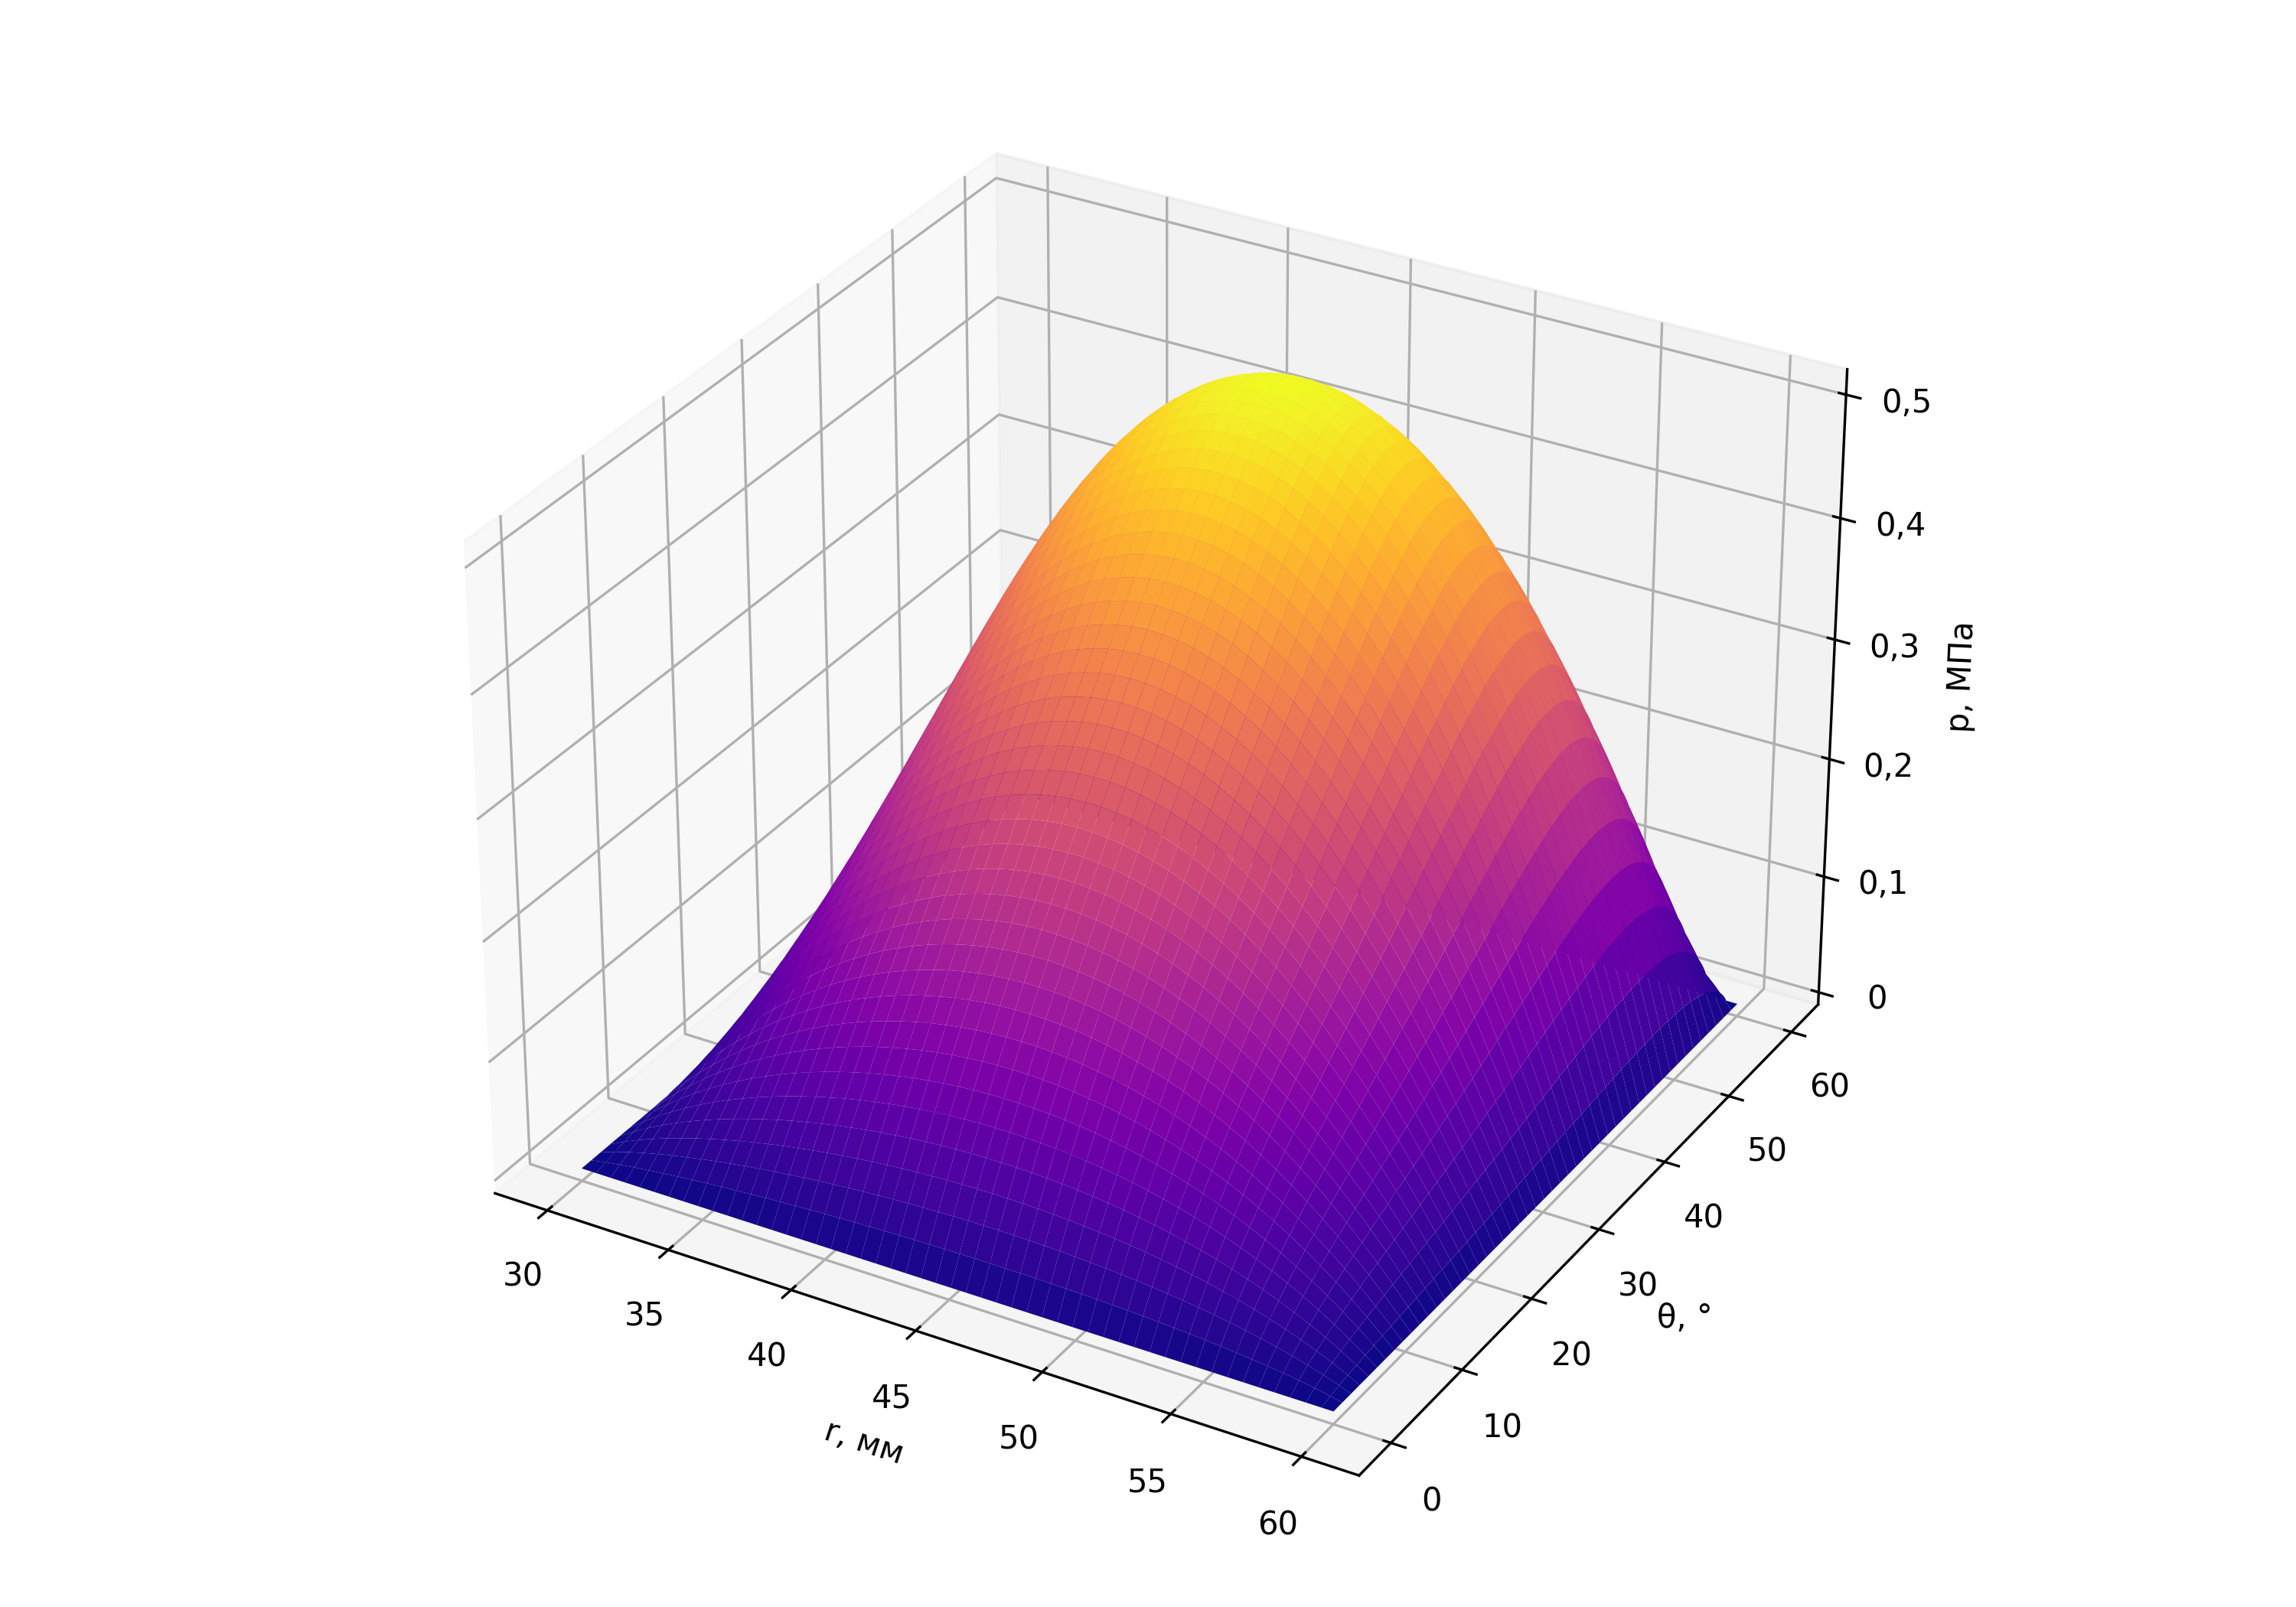
\includegraphics[width=\textwidth,height=0.9\textheight,keepaspectratio]{figures/ch07/fig_7_8.png}
\caption{Поле давления $p(r, \theta)$ гладкого подшипника
  при $K_{\mathrm{nom}} = 2{,}0$.}
\label{fig:thrust_P3D_smooth}
\end{figure}

\FloatBarrier

\textit{Конфигурация~T2.}
Текстурирование поверхности по конфигурации~T2 приводит к появлению
локальных пиков давления над лунками во входной и средней части
сектора (<<рябь>> на поверхности $p(r, \theta)$, рис.~\ref{fig:thrust_P3D_T2}). Интегральная
несущая сила возрастает вследствие дополнительных гидродинамических
клиньев, формируемых передними стенками лунок. В выходной части
сектора ($\theta > 0{,}7\beta$), свободной от текстуры, профиль
давления близок к гладкому случаю.

\begin{figure}[!ht]
\centering
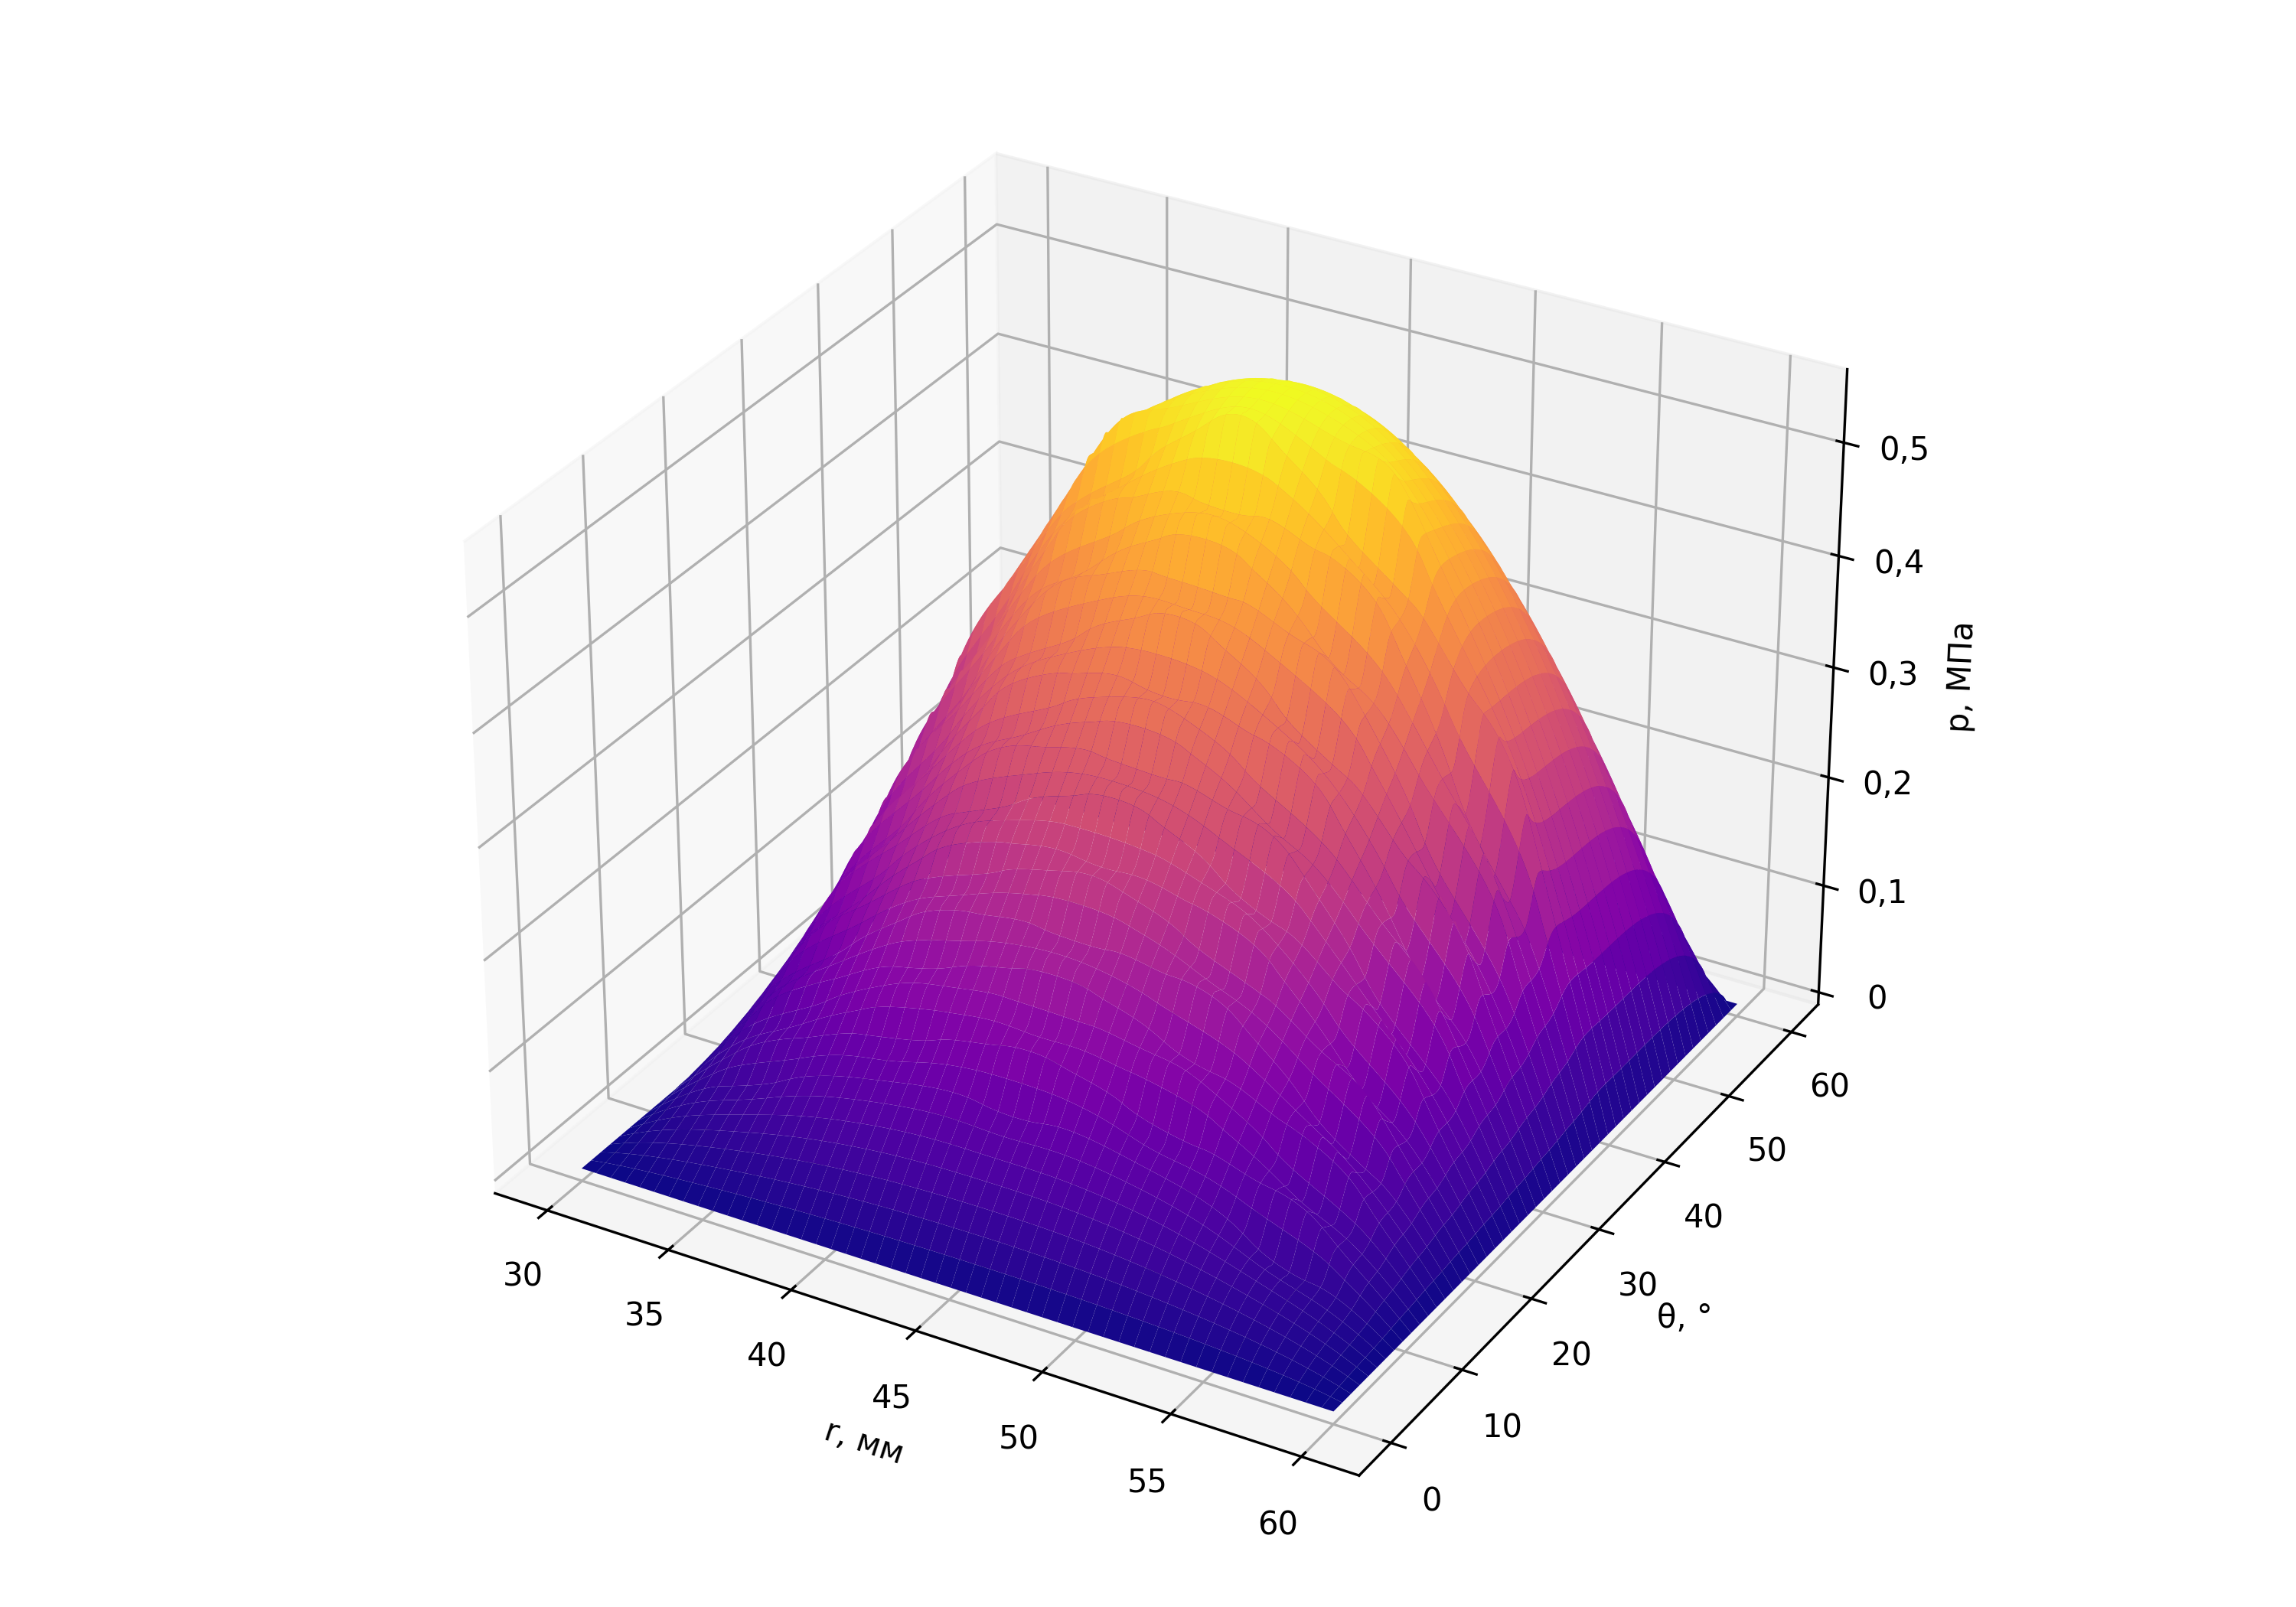
\includegraphics[width=\textwidth,height=0.9\textheight,keepaspectratio]{figures/ch07/fig_7_9.png}
\caption{Поле давления $p(r, \theta)$ для конфигурации~T2
  ($H_p = 0{,}40$, зона $0{,}1\beta$--$0{,}7\beta$)
  при $K_{\mathrm{nom}} = 2{,}0$.}
\label{fig:thrust_P3D_T2}
\end{figure}

\FloatBarrier

\textit{Конфигурация~T3.}
Конфигурация~T3 располагает лунки в средней и выходной части клина,
где зазор мал и давление убывает. В этой зоне передние стенки лунок
не создают эффективного гидродинамического клина; напротив, нарушение
плавности зазора в зоне убывающего давления снижает интегральную
несущую силу ниже уровня гладкого варианта ($G_W = 0{,}9816$).

\FloatBarrier
\section*{Выводы по главе~7}
\phantomsection\addcontentsline{toc}{section}{Выводы по главе~7}

Разработана численная модель упорного подшипника скольжения
с секторными колодками и детерминированными микроструктурами
рабочей поверхности~\cite{suh2015a,suh2015b,yang2021,song2024}. Модель основана на цилиндрической форме
уравнения Рейнольдса~\eqref{eq:thrust_reynolds}, решаемого
методом SOR на равномерной сетке $200 \times 300$ с обнулением
отрицательных давлений.

Проведён сравнительный расчёт гладкого варианта и конфигураций
T1, T2, T3 при $K_{\mathrm{nom}} = 2{,}0$. Установлено, что
текстурирование во входной и средней части клина (T1,~T2)
обеспечивает умеренный рост несущей способности и снижение
коэффициента трения. Наилучшие показатели у конфигурации~T2:
$G_W = 1{,}0145$, $G_{f_T} = 1{,}0337$.

Смещение текстуры в среднюю и выходную часть сектора (T3)
оказывается неэффективным: $G_W = 0{,}9816 < 1$, что подтверждает
определяющую роль зоны нанесения текстуры относительно зоны
нарастания давления.

Рост несущей способности при T1 и~T2 сопровождается увеличением
утечек смазочного материала ($G_Q = 0{,}9847$ и $0{,}9733$)
и максимального давления в плёнке ($G_{p_{\max}} = 0{,}9517$
и $0{,}9228$). Данный компромисс необходимо учитывать при выборе
конфигурации рабочей поверхности.

Параметрический расчёт по
$K \in [1{,}5;\; 4{,}0]$ показал, что несущая сила имеет максимум
при $K \approx 2{,}5$ для всех вариантов; коэффициент трения
монотонно убывает с ростом~$K$. Преимущество~T2 по несущей
способности сохраняется по всему исследованному диапазону~$K$.

Результаты анализа упорного подшипника дополняют результаты
глав~5 и~6, расширяя область применения детерминированных
микроструктур на подшипники с клиновым зазором.

